


% {}\documentclass[a4paper,landscape,twoside]{article}
% {}\documentclass[a4paper,landscape,10pt]{article}

{}\documentclass[a4paper]{article}
% {}\documentclass[a4paper,landscape]{article}


%-----------------------------------------------------------------
% GENERAL PACKAGES
%-----------------------------------------------------------------
\RequirePackage[ddmmyyyy]{datetime} % change date format
\renewcommand{\dateseparator}{.} % select date separator character
\RequirePackage[shortlabels]{enumitem} % pause/resume lists
\RequirePackage{multicol} % multi column format
\RequirePackage{graphicx} % used for figures
% \graphicspath{{images/}} % put figures inside folder 'images'  in same folder as .tex %%% why? do? TODO
\RequirePackage[dvipsnames]{xcolor} %colors, dvips -> extra premade colors
\RequirePackage[explicit]{titlesec} % formating of titles
% \RequirePackage{amssymb}
\RequirePackage{siunitx} % SI units
\usepackage{amsmath, amssymb} % For mathematical symbols and equations
% \RequirePackage{amsfonts} % more math stuff
\RequirePackage{mathtools} % even more math stuff
\RequirePackage{empheq} % Fancy boxed equations
\RequirePackage{fancybox} % Additional box types
\RequirePackage{subcaption}
\RequirePackage[hidelinks]{hyperref} % used for hyperlinked nodes
% \usepackage{hyperref} % For hyperlinks
\RequirePackage[document]{ragged2e} % left ragged text
\RequirePackage{atbegshi}  % special commands that apply tikz to all pages
\RequirePackage{fancyhdr} % custom header/footer
\RequirePackage{etoolbox} % Boolean and if/else
\RequirePackage{calc} % math inside other commands
\RequirePackage{booktabs}

\RequirePackage{multirow}

\usepackage{parskip} % For paragraph spacing

\usepackage{lipsum} % For dummy text (can be removed)
\usepackage[ngerman]{babel}

\usepackage{lmodern}
\usepackage{longtable}
%=================================================================
% O P T I O N S   S T A R T
%=================================================================

%-----------------------------------------------------------------
% GEOMETRY OPTIONS
%-----------------------------------------------------------------

\newlength{\paperh}
\newlength{\paperw}
\newlength{\inmar}
\newlength{\outmar}
\newlength{\topmar}
\newlength{\botmar}
\newlength{\footmar}


\DeclareOption{a4standard}{
    \setlength\paperh{297mm}
    \setlength\paperw{210mm}
    \setlength\inmar{20mm}
    \setlength\outmar{20mm}
    \setlength\topmar{20mm}
    \setlength\botmar{20mm}
    \setlength\footmar{12mm}
}

\DeclareOption{a4compact}{
    \setlength\paperh{297mm}
    \setlength\paperw{210mm}
  \setlength\inmar{1mm}
    \setlength\outmar{1mm}
    \setlength\topmar{1mm}
    \setlength\botmar{1mm}
    \setlength\footmar{5mm}
}

\DeclareOption{a3compact}{
    \setlength\paperh{420mm}
    \setlength\paperw{297mm}
    \setlength\inmar{1mm}
    \setlength\outmar{1mm}
    \setlength\topmar{1mm}
    \setlength\botmar{1mm}
    \setlength\footmar{5mm}
}

%-----------------------------------------------------------------
% COLOR OPTIONS
%-----------------------------------------------------------------
% color1 - main color
% color2 - Blue color
% color3 - Highlight color

\DeclareOption{colorful}{
    \colorlet{color1}{black}
    \colorlet{color2}{NavyBlue}
    \definecolor{color3}{HTML}{FFE534} % bf2042yellow
}

\DeclareOption{b/w}{
    \colorlet{color1}{black}
    \colorlet{color2}{black}
    \colorlet{color3}{black!20}
}

%=================================================================
% PROCESS OPTIONS
%=================================================================
\ExecuteOptions{a4standard, colorful}
\ProcessOptions\relax

%%%%%%%%%%%%%%%%%%%%%%%%%%%%%%%%%%%%%%%%%%%%%%%%%%%%%%%%%%%%%%%%%%
% O P T I O N S   E N D
%%%%%%%%%%%%%%%%%%%%%%%%%%%%%%%%%%%%%%%%%%%%%%%%%%%%%%%%%%%%%%%%%%

%%%%%%%%%%%%%%%%%%%%%%%%%%%%%%%%%%%%%%%%%%%%%%%%%%%%%%%%%%%%%%%%%%
% GLOBAL FORMATTING
%%%%%%%%%%%%%%%%%%%%%%%%%%%%%%%%%%%%%%%%%%%%%%%%%%%%%%%%%%%%%%%%%%

\RequirePackage[utf8]{inputenc} % more charecter inpus (ü,ö,ä)
\RequirePackage[T1]{fontenc}
\RequirePackage{helvet}
\renewcommand{\familydefault}{\sfdefault}

\RequirePackage[
    paperheight=\paperh,
    paperwidth=\paperw,
    margin=0.1cm,
    top=\topmar,
    bottom=\botmar,
    headsep=0.5cm,
    headheight=0.5cm,
    footskip=\footmar,
    inner=\inmar,
    outer=\outmar,
    centering
]{geometry}

%-----------------------------------------------------------------
% GLOBAL PARAMETER COMMANDS
%-----------------------------------------------------------------
\pagestyle{fancy}
\fancyhf{}
\fancyfoot[C]{Seite \thepage}

%-----------------------------------------------------------------
% OTHER FORMATTING
%-----------------------------------------------------------------
%indent for paragraph
\setlength{\parindent}{0pt}
%space between paragraphs
\setlength{\parskip}{0.3em}

%space between columns
\setlength{\columnsep}{0.2cm}
% create lines between columns and define color of columns
\setlength{\columnseprule}{1pt} %set thickness default 1pt
\def\columnseprulecolor{\color{black}}

% spacing within lists
\setlist[enumerate]{nosep}
\setlist[itemize]{nosep}
\setlist[description]{nosep}

%-----------------------------------------------------------------
% Kaptielnummmer
%-----------------------------------------------------------------
  \usepackage{sectsty}
  % \sectionfont{\clearpage\Large\bfseries} % Top-level section (unnumbered)
  \setcounter{secnumdepth}{2} % Number subsections (##)
  % \setcounter{tocdepth}{2} % Include subsections in TOC
  \renewcommand{\thesubsection}{\arabic{subsection} } % Number subsections as 1., 2., etc.
%-----------------------------------------------------------------
  \setlist[itemize]{leftmargin=4mm}

%command for tight list 
\providecommand{\tightlist}{\setlength{\itemsep}{1mm}\setlength{\parskip}{1mm}}

% image 
\let\oldincludegraphics\includegraphics
\renewcommand{\includegraphics}[2][]{\oldincludegraphics[#1, width=0.7\textwidth, keepaspectratio]{#2}}



%-----------------------------------------------------------------
% INHALT
%-----------------------------------------------------------------

\begin{document}

% \begin{multicols}{1}

\begin{center}
	%-----------------------------------------------------------------
	\LARGE \textbf{\colorbox{RoyalBlue}{\textcolor{white}{Strategische Studien II}}} \\
	\normalsize
	\textbf{\colorbox{lightgray}{\textcolor{Black}{Silvan Stadelmann} \url{silvasta@ethz.ch}}}\\
	\today{}
	\footnotesize
	%-----------------------------------------------------------------
\end{center}

\tableofcontents

\section{Strategische Studien II}\label{strategische-studien-ii}

Militärakademie (MILAK) an der ETH Zürich\\
Vorlesung Strategische Studien II\\
Dr.~Marcel Berni

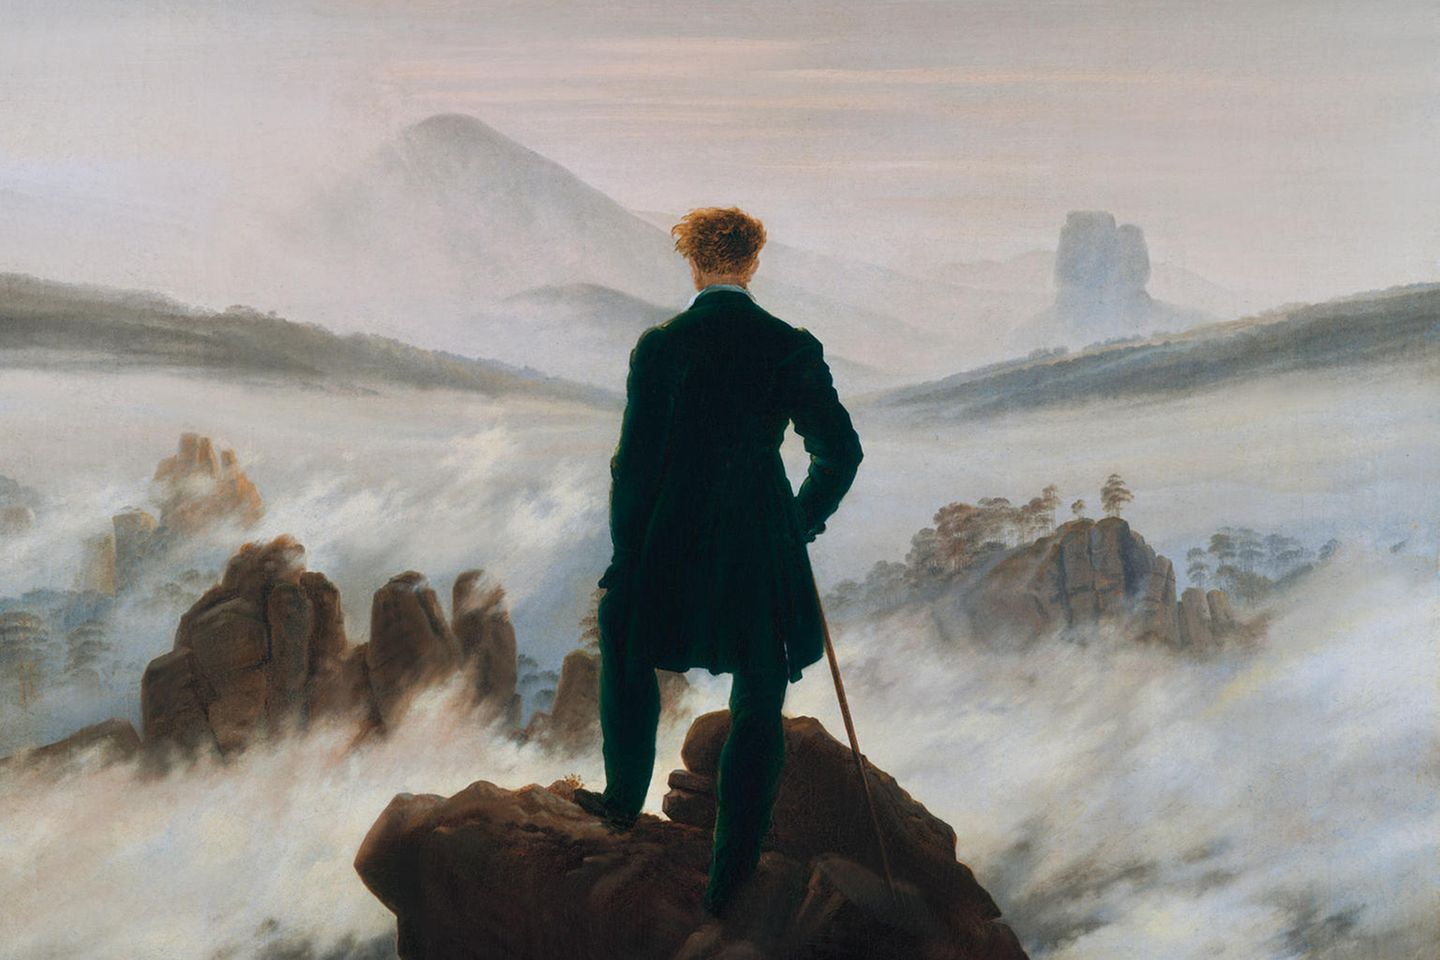
\includegraphics{images/wanderer.jpg} \emph{Der Wanderer über dem
	Nebelmeer Caspar David Friedrich, 1818}

\subsection{Einleitung}\label{einleitung}

\subsubsection{Lernziele}\label{lernziele}

\begin{itemize}
	\item
	      Die Studierenden kennen wirkmächtige Konzepte (militär-)strategischer
	      Theorie und Praxis. Sie lernen, wie sich das Verständnis von Strategie
	      über die Zeit verändert hat.
	\item
	      Die Studierenden können aktuelle Kriege und Konflikte aus
	      verschiedenen Perspektiven einordnen und die jeweils verfolgten Ziele
	      der verschiedenen Akteure diskutieren.
	\item
	      Die Studierenden können die in der Vorlesung behandelten Theorien und
	      Fallbeispiele miteinander vergleichen und gegebenenfalls zueinander in
	      Beziehung setzen. Zudem lernen sie, Originaltexte und
	      Fachpublikationen auf dem Gebiet der Strategischen Studien kritisch zu
	      hinterfragen.
\end{itemize}

\subsubsection{Strategie, Operation und
	Taktik}\label{strategie-operation-und-taktik}

\begin{figure}
	\centering
	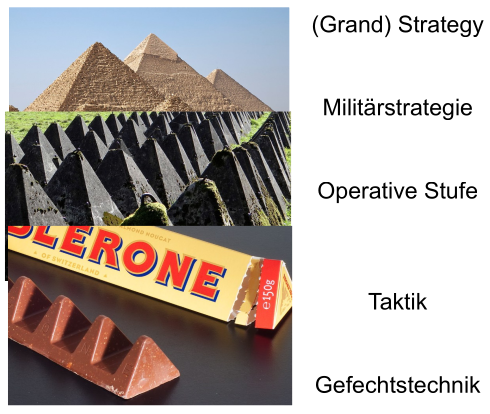
\includegraphics{images/strategie-pyramide.png}
	\caption{Strategie Pyramide}
\end{figure}

\begin{quote}
	Mit Taktik gewinnt man das Gefecht, mit Operationen einen Feldzug und
	mit Strategie einen Krieg.\\
	- \emph{Gustav Däniker, Schweizerische Selbstbehauptungsstrategie im
		Kalten Krieg, Frauenfeld 1996}
\end{quote}

\subsubsection{Strategie und
	Theoriebildung}\label{strategie-und-theoriebildung}

\begin{quote}
	In theory there is no difference between theory and practice. In
	practice there is.\\
	- \emph{Strategic Theory for the 21st Century: The Little Book on Big
		Strategy 2006}
\end{quote}

\begin{quote}
	Strategic theory in the real world confronts the dynamic nature of the
	strategic environment and the mind of the strategist - how strategists
	approach strategy-making in the context of their strategic environments.
	{[}\ldots{]} Good strategy flows from understanding the nature of the
	environment and creating a symmetry and synergy of objectives, concepts,
	and resources that offer the best probability of achieving the policy
	aims. The strategist is assisted by the logic of strategy and the
	construct of planning, but the strategist is not a planner.\\
	- \emph{Harry R. Yarger, Strategic Theory for the 21st Century: The
		Little Book on Big Strategy, Carlisle 2006}
\end{quote}

\begin{quote}
	Theory provides guidance for what usually would be sound behavior, but,
	as well as a gamble, war is also an environment wherein exceptions can
	and do occur.\\
	- \emph{Colin S. Gray, Theory of Strategy, Oxford 2018}
\end{quote}

\subsubsection{Gray, Modern Strategy, Oxford
	1999}\label{gray-modern-strategy-oxford-1999}

\begin{quote}
	Overall, strategy is where policy meets the battlespace {[}\ldots{]} On
	the strategy bridge, the strategist must translate political desires
	into plans for their realization. {[}\ldots{]} Strategy is only the
	bridge connecting the world of tactical engagement with that of
	political purpose.\\
	- \emph{Colin S. Gray, Fighting Talk. Forty Maxims on War, Peace, and
		Strategy, Westport-London 2007}
\end{quote}

\begin{itemize}
	\tightlist
	\item
	      Krieg und Strategie als ganzheitliches Phänomen: 17 Dimensionen in 3
	      Clustern
	\item
	      Dimensionen zeitlos gültig, Wirkung variiert je nach Konflikt, deshalb
	      keine Hierarchisierung
	\item
	      Bedeutung der Dimensionen

	      \begin{itemize}
		      \tightlist
		      \item
		            Exzellenz in allen Dimensionen nicht notwendig (Möglichkeit zur
		            Kompensation)
		      \item
		            Dramatische Verbesserung in einem oder zwei Bereichen garantieren
		            keinen strategischen Erfolg
		      \item
		            Katastrophale Schwäche in einzelner Kategorie kann tödlich sein
	      \end{itemize}
	\item
	      Der Master Stratege beherrscht alle Dimensionen.
\end{itemize}

\paragraph{People and Politics}\label{people-and-politics}

\subparagraph{People}\label{people}

\subparagraph{Society}\label{society}

\subparagraph{Culture}\label{culture}

\subparagraph{Politics}\label{politics}

\subparagraph{Ethics}\label{ethics}

\paragraph{Preparation of War}\label{preparation-of-war}

\subparagraph{Economics and Logistics}\label{economics-and-logistics}

\subparagraph{Organization (incl.~Defence and force
	planning)}\label{organization-incl.-defence-and-force-planning}

\subparagraph{Military administration (incl.~Recruitment, Training,
	Armaments)}\label{military-administration-incl.-recruitment-training-armaments}

\subparagraph{Information and
	Intelligence}\label{information-and-intelligence}

\subparagraph{Strategic Theory and
	Doctrine}\label{strategic-theory-and-doctrine}

\subparagraph{Technology}\label{technology}

\paragraph{War Proper}\label{war-proper}

\subparagraph{Military Operations}\label{military-operations}

\subparagraph{Command (political and
	military)}\label{command-political-and-military}

\subparagraph{Geography}\label{geography}

\subparagraph{Friction (incl.~chance and
	uncertainty)}\label{friction-incl.-chance-and-uncertainty}

\subparagraph{Adversary}\label{adversary}

\subparagraph{Time}\label{time}

\subsubsection{Mittel, Wege und Ziele}\label{mittel-wege-und-ziele}

\begin{figure}
	\centering
	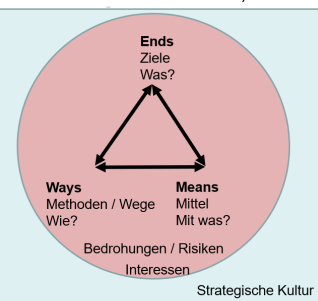
\includegraphics{images/ways-means-ends.png}
	\caption{ways-means-ends}
\end{figure}

\begin{quote}
	Strategy equals ends (objectives toward which one strives) plus ways
	(courses of action) plus means (instruments by which some end can be
	achieved).\\
	- \emph{Arthur F. Lykke, Towards an Understanding of Military Strategy,
		1984--1985}
\end{quote}

\subsubsection{Modernes
	Strategieverständnis}\label{modernes-strategieverstuxe4ndnis}

Wie erreicht man seine Ziele gegen einen (bewaffneten) Gegner?

\begin{itemize}
	\tightlist
	\item
	      (Politische) Festlegung und Verfolgung eines Ziels
	\item
	      Formulierung und Anwendung eines Plans, unter Berücksichtigung des
	      Gegners und Hindernisse
	\item
	      Einsatz offener und verdeckter (Macht-)Mittel, Methoden und Wege
\end{itemize}

\begin{quote}
	\textbf{Eine Strategie ist ein Plan über den Mitteleinsatz zur
		Zielerreichung unter Berücksichtigung der gegnerischen Strategie sowie
		externer Faktoren.}
\end{quote}

\subsubsection{Methodische
	Grundprobleme}\label{methodische-grundprobleme}

\begin{itemize}
	\tightlist
	\item
	      Informationsbasis und deren Messbarkeit: keine exakten Daten für die
	      Vergangenheit, nur Annahmen für die Zukunft
	\item
	      Veränderlichkeit der Komponenten (z.B. Ziele, Wege, Mittel) im
	      Untersuchungszeitraum
	\item
	      Interaktion mit dem Gegenspieler (mit eigener Strategie und Friktion)
	\item
	      Deklaration und Aktion: Notwendigkeit der Unterscheidung
	\item
	      Erfolgsmassstab: abhängig von Beobachter und Zeitpunkt
\end{itemize}

\subsubsection{Repetition SSI}\label{repetition-ssi}

\begin{itemize}
	\tightlist
	\item
	      Begriffe ``Strategie'' und ``Taktik'' sind antik (5. Jh. v. Chr.),
	      aber nur Taktik ist damals gebräuchlich.
	\item
	      ``Strategie'' kommt Ende 18. Jh. in Gebrauch.
	\item
	      Strategie und Taktik sind ursprünglich geographisch voneinander
	      getrennt. Allmählich kommt eine hierarchische Trennung hinzu, in
	      welche sich im 20. Jahrhundert die ``operative Stufe'' einfügt.
	\item
	      Die Diskussion, ob Strategie eine Wissenschaft, eine Kunst oder ein
	      Plan ist, ist bis heute nicht entschieden. Es gibt verschiedene Formen
	      der Visualisierung von Strategien.
	\item
	      Ab Mitte 20. Jh. wird ``Strategie'' zunehmend der politischen Führung
	      zugeordnet, während die militärische Führung nur noch für
	      ``Operationsführung'' und Taktik zuständig ist.
	\item
	      In den 1960er Jahren übernehmen die Wirtschaftswissenschaften das
	      Konzept der Strategie.
	\item
	      Der heutige Sprachgebrauch ist kontextabhängig und mitunter beliebig.
	\item
	      Das Adjektiv ``strategisch'' wird oft synonym mit ``auf oberster
	      Stufe'', ``umfassend'', ``langfristig'' oder ``überragend wichtig''
	      verwendet. Bei Waffensystemen wird damit die Reichweite bezeichnet.
\end{itemize}

\paragraph{Kriegsursachen, Siegestheorien und
	Kriegsbeendigung}\label{kriegsursachen-siegestheorien-und-kriegsbeendigung}

\begin{itemize}
	\tightlist
	\item
	      Thukydides: Angst/Furcht, Ehre/Ehrgeiz, Interessen/Gier als
	      Kriegsursachen, Unterscheidung Kriegsursachen vs.~Kriegsgründe
	\item
	      Clausewitz: Krieg als Chamäleon das zwischen Regierung, Volk,
	      Feldherr/Heer mit jeweils unterschiedlichen Attributen oszilliert,
	      Krieg als einfacher oder erweiterter Ringkampf
	\item
	      Bartholomees: Kontinuum Sieg von Sieg zu Niederlage, Taktische und
	      operative Erfolge resultieren nicht automatisch in strategischem Sieg!
	      Decisiveness und Achievement als Indikatoren
	\item
	      Lee/McDonnell: Resultatorientierte Siegestheorie, die gewisse
	      Kriegsausgänge (z.B. Patt) marginalisiert.
\end{itemize}

\paragraph{Der Indirekte Ansatz}\label{der-indirekte-ansatz}

\begin{itemize}
	\tightlist
	\item
	      Indirekter Ansatz als Gegenstück zum Frontalangriff, Ausgerichtet auf
	      Schwachpunkte des Gegners, Umgehung seiner Stärken
	\item
	      Zwei Grundformen (kriegsverkürzend/kriegsverlängernd) mit
	      unterschiedlichen Zielen, Vorgehensweisen und Anforderungen,
	      Gemeinsamkeit: Sieg ohne Schlacht
	\item
	      Kann zahlenmässige bzw. materielle Unterlegenheit wettmachen, aber mit
	      Risiken verbunden
\end{itemize}

\paragraph{Strategien im napoleonischen
	Zeitalter}\label{strategien-im-napoleonischen-zeitalter}

\begin{itemize}
	\tightlist
	\item
	      Jomini: Grosser Einfluss auf Denken und Operationsführung in USA bis
	      1861/65, bei europäischen Armeen bis 1914
	\item
	      Clausewitz: Grosser Einfluss auf strategisches Denken im 20./21.
	      Jahrhundert
	\item
	      Jomini: Suche nach ``ewigen'' Prinzipien und Regeln
	\item
	      Jomini's Abriss der Kriegskunst hat den Amerikanern die französische
	      Doktrin erschlossen, und zwar für terrestrische, maritime und
	      amphibische Operationen sowie die Rolle der Logistik
	\item
	      Clausewitz: Dynamik, Dialektik, Irrationalität, höhere Gewalt (force
	      majeure)
	\item
	      Rezeption: ``Inflation'' technischer Begriffe mit teilweise unscharfer
	      Definition und in schwankender Verwendung
\end{itemize}

\paragraph{Clausewitz: Friktion, Schwerpunkt und
	Kulminationspunkt}\label{clausewitz-friktion-schwerpunkt-und-kulminationspunkt}

\begin{itemize}
	\tightlist
	\item
	      Unterscheidung absoluter/wirklicher Krieg, letzterer geprägt von
	      politischem Zweck und Friktion
	\item
	      Faktor Mensch (Intuition, Erfahrung, Moral etc.) entscheidend bei
	      Clausewitz
	\item
	      Friktion allgegenwärtig, moderne Technologie bietet gewisse Abhilfe,
	      schafft zugleich aber neue Anfällig- und Abhängigkeiten
	\item
	      Unterschiedliches Verständnis bzw. Konzeption von Schwerpunkt/Center
	      of Gravity
	\item
	      Kulmination aus Kombination verschiedener Faktoren, erfordert
	      sorgfältige Planung und Flexibilität
\end{itemize}

\paragraph{Simulation, Kriegsspiel und Operations
	Research}\label{simulation-kriegsspiel-und-operations-research}

\begin{itemize}
	\tightlist
	\item
	      Verschiedenste Formen der Modellierung und militärischen Simulation
	\item
	      Ziel: Entscheidungen auf allen Stufen spielerisch simulieren
	\item
	      (Preussisches) Kriegsspiel setzt sich im 19. Jahrhundert durch
	\item
	      Weiterentwicklungen: Operations Research, Lanchester's laws, Tactical
	      Numerical Deterministic Model, Sigma War Games
	\item
	      Ambivalenter Einsatz in Vergangenheit und Aktualität
	\item
	      Interdisziplinäre Befruchtung, keine disziplinäre Vormachtstellung
	\item
	      Enge Zusammenarbeit zwischen militärischen und zivilen Stellen
	\item
	      Aktuell: Simulationen wieder im Trend
	\item
	      Zukunft: Computerisierung und AI
\end{itemize}

\paragraph{Allianzen, Kooperationen und Gleichgewicht der
	Kräfte}\label{allianzen-kooperationen-und-gleichgewicht-der-kruxe4fte}

\begin{itemize}
	\tightlist
	\item
	      Allianzen und Bündnisse als zeitlose Problemstellung -- Abwägung von
	      Kosten und Nutzen, Vor- und Nachteilen
	\item
	      Tendenz zu ad-hoc Koalitionen angesichts neuem Grossmachtwettbewerb
	      möglicherweise wieder rückläufig
	\item
	      NATO als Sonderfall, aber mit ungewisser Zukunft
	\item
	      Kooperation mit und unter nicht-staatlichen Akteuren mit denselben
	      Logiken und Dynamiken
\end{itemize}

\paragraph{Überraschung, Täuschung,
	Nachrichtendienst}\label{uxfcberraschung-tuxe4uschung-nachrichtendienst}

\begin{itemize}
	\tightlist
	\item
	      Militärische Überraschung und Täuschung als potenzielle
	      Kräftemultiplikatoren, allerdings oft mit nicht beabsichtigten
	      Nebeneffekten
	\item
	      Täuschung letztlich kognitives Phänomen, bedingt vertiefte Kenntnisse
	      der anderen Seite
	\item
	      Nachrichtendienstliches Versagen vielschichtig, vermutlich auch in
	      Zukunft unvermeidlich
\end{itemize}

\paragraph{Der Einfluss von Kultur und
	Technologie}\label{der-einfluss-von-kultur-und-technologie}

\begin{itemize}
	\tightlist
	\item
	      Konzept der strategischen Kultur wird wichtiger in den Strategischen
	      Studien, Operationalisierung, Definition und Methodik bleiben jedoch
	      heterogen
	\item
	      Strategische Kultur als ergänzender Erklärungsansatz für Unterschiede
	      zwischen Armeen und Militärbürokratien
	\item
	      Konnex zwischen strategischer Kultur und militärtechnologischem
	      Einsatz evident, iterative Beeinflussung
	\item
	      Entwicklung neuer Waffensysteme benötigt viel Zeit, Geld und Personal.
	      Gleichwohl sind sie für Staaten von strategischer Bedeutung
	\item
	      Aktuelle Forschung stellt RMA als dominanter Erklärungsansatz vermehrt
	      in Frage
\end{itemize}

\paragraph{Seekriegführung}\label{seekriegfuxfchrung}

\begin{itemize}
	\tightlist
	\item
	      Sea Control/Sea Denial bzw. Nutzung SLOCs als anhaltende
	      Grundherausforderung maritimer Strategie und Seekriegführung
	\item
	      Klassische Rollen Seestreitkräfte mehrheitlich fortbestehend bei
	      gleichzeitiger Erweiterung Missionsspektrum
	\item
	      Uneingeschränkte Dominanz US-Navy künftig vermutlich zunehmend infrage
	      gestellt
\end{itemize}

\paragraph{Luftkriegführung}\label{luftkriegfuxfchrung}

\begin{itemize}
	\tightlist
	\item
	      Potenzial Luftkriegsführung und Luftmacht frühzeitig erkannt, Wirkung
	      von strategischen Bombardierungen aber über- und Luftverteidigung
	      unterschätzt
	\item
	      Debatte um effektivste Anwendung (strategisch vs.~taktisch-operativ)
	      weiter anhaltend
	\item
	      Air Power wirksam und unabdingbar im Verbund, kann bewaffnete
	      Konflikte aber nicht im Alleingang entscheiden
	\item
	      Aktuelle Drohnengeneration noch kein Ersatz für Kampfflugzeuge, aber
	      nächste Generation bereits in Entwicklung
\end{itemize}

\paragraph{Landkriegsführung}\label{landkriegsfuxfchrung}

folgt\ldots{}

\paragraph{Nuklearstrategie \&
	Massenvernichtungswaffen}\label{nuklearstrategie-massenvernichtungswaffen}

\begin{itemize}
	\tightlist
	\item
	      Hoch hypothetische Wissenschaft (zum Glück!)
	\item
	      Abschreckung als zentrales Element
	\item
	      Wechselseitige Interaktion, Kommunikation über Absichten entscheidend
	\item
	      Spezifische Denkfiguren und Paradoxien

	      \begin{itemize}
		      \tightlist
		      \item
		            garantierte Zweitschlagfähigkeit sorgt für Stabilität
		      \item
		            Irrationalität erhöht Glaubwürdigkeit
		      \item
		            Extended Deterrence
	      \end{itemize}
	\item
	      Basiert nur auf theoretischen Annahmen
	\item
	      Stigmatisierung von Kernwaffen betrifft Demokratien, nicht aber
	      Diktaturen
	\item
	      Besteht das nukleare Tabu auch im zweiten Nuklearzeitalter?
\end{itemize}

\subsection{Joint Warfare}\label{joint-warfare}

Wirkungsraumübergreifende Kriegführung

\subsubsection{Leitfragen}\label{leitfragen}

\begin{itemize}
	\tightlist
	\item
	      Welche strategischen Konzeptionen wirkungsraumübergreifender
	      Kriegführung gibt es?
	\item
	      Wie gestaltet sich der Kampf der verbundenen Kräfte in der
	      wirkungsraumübergreifenden Kriegführung?
	\item
	      Welchen Herausforderungen sieht sich die wirkungsraumübergreifende
	      Kriegführung ausgesetzt?
\end{itemize}

\subsubsection{Lektüre}\label{lektuxfcre}

\begin{itemize}
	\tightlist
	\item
	      Hew Strachan, One War, Joint Warfare, in: The RUSI Journal, Vol. 154
	      (4), 2009, S. 20-24.
	\item
	      Edward R. Lucas/Thomas A. Crosbie, Evolution of Joint Warfare, in:
	      Anders McD Sookermany (Hg.), Handbook of Military Sciences, online
	      first, \url{https://doi.org/10.1007/978-3-030-02866-4_21-1}.
\end{itemize}

\subsubsection{Begriffsverwendung}\label{begriffsverwendung}

Es gibt keine klare Definition und vielfach unterschiedliche Verwendung
des Begriffs.

\begin{itemize}
	\tightlist
	\item
	      Kampf / Gefecht der verbundenen Kräfte / Waffen
	\item
	      Multi / All Domain Operations
	\item
	      Joint Warfare
	\item
	      Cross Domain Operations
	\item
	      Integrated Operations
	\item
	      Network-centric Warfare
	\item
	      Effects-based Operations
	\item
	      Comprehensive Approach
	\item
	      Distributed Operations
	\item
	      Cyber-physical Operations
	\item
	      Full spectrum warfare
\end{itemize}

Wir definieren die wirkungsraumübergreifende Kriegsführung als
koordinierte militärische Operationen verschiedener Teilstreitkräfte,
die zwei oder mehr Operationsräume miteinander verbinden.

\subsubsection{Anfänge}\label{anfuxe4nge}

\begin{itemize}
	\tightlist
	\item
	      Französische und deutsche Offiziere versuchten im 1. WK Schützengräben
	      zu überwinden
	\item
	      Stosstrupps, flexible Flächenverteidigung und später Panzerwaffe
	\item
	      Kommunikation zwischen unterschiedlichen Waffengattungen (primär
	      Artillerie und Infanterie)
	\item
	      Ziel: Synchronisation und Steigerung der Feuerkraft und Bewegung
	\item
	      Flankierung durch Keilformationen und Kesselbildungen
	\item
	      Erweiterung im 2. WK um Flugzeuge, Flugabwehr, Panzer
	\item
	      Später: Elektromagnetische Kriegführung, Cyber und Krieg im All
\end{itemize}

\subsubsection{AirLand Battle (1982/86)}\label{airland-battle-198286}

\begin{itemize}
	\tightlist
	\item
	      Offensive Ausrichtung, Manöver statt Abnutzung,
	      Follow-on-Forces-Attack, Deep Attack
	\item
	      Extended Battlefield durch Kampf der verbundenen Waffen und
	      Synchronisierung von:

	      \begin{itemize}
		      \tightlist
		      \item
		            Close Operations
		      \item
		            Deep Operations
		      \item
		            Rear Operations
	      \end{itemize}
	\item
	      Erlangung Initiative durch Tempo, Überraschung und Täuschung sowie
	      Flexibilität
	\item
	      Bezüge zu Clausewitz (Center of Gravity, Culminating Point)
	      /Liddell-Hart (Indirect Approach)
	\item
	      Paradebeispiel ``Desert Storm'' (1991)
\end{itemize}

\subsubsection{Network-centric warfare und Effects-based
	Operations}\label{network-centric-warfare-und-effects-based-operations}

Denkmethodik: Effekte - Systemanalyse - Wahl der Mittel aus gesamtem
Spektrum, fein dosiert und mit Priorisierung der zivilen/psychologischen
Mittel

\begin{itemize}
	\tightlist
	\item
	      Zentrale Stellung in US- und NATO-Doktrinen
	\item
	      Schmale empirische Basis für Überprüfung
	\item
	      Technologiegläubigkeit
	\item
	      Anfälligkeit für übersetzte Erwartungen
\end{itemize}

\subsubsection{Effects-based Operations}\label{effects-based-operations}

\begin{quote}
	Any political entity can be thought of as a system consisting of a
	number of subsystems, or to borrow a term coined in the former Air Force
	Systems command -- a system of systems.
\end{quote}

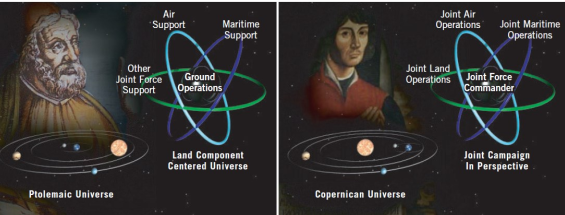
\includegraphics{images/kopernikus.png}\\
\emph{Vergleich mit Entdeckung der tatsächlichen funktionsweise der
	Umlaufbahn}

\begin{quote}
	Effective control of enough of the adversary's enabling operation level
	systems will paralyse his ability to function at the strategic level.\\
	- \emph{David A. Deptula, Effects-based Operations: Change in the Nature
		of War, Arlington 2001.}
\end{quote}

\subsubsection{Multi Domain Operations
	(2016)}\label{multi-domain-operations-2016}

Neuausrichtung von Aufstandsbekämpfung auf konventionellen Gegner mit
fortschrittlichen Fähigkeiten insbesondere im Bereich A2AD (anti-access,
area denial)

Unterschied zu Joint Operations: MDO inkludiert nicht-militärische
Assets

\begin{itemize}
	\tightlist
	\item
	      Veränderte Bedrohungslage

	      \begin{itemize}
		      \tightlist
		      \item
		            Neue chinesische Bedrohung
		      \item
		            Krim-Besetzung 2014
		      \item
		            Tendenz zu neuem Grossmachtwettbewerb
	      \end{itemize}
	\item
	      Abfolge MDO:

	      \begin{itemize}
		      \tightlist
		      \item
		            Penetrate
		      \item
		            Dis-integrate
		      \item
		            Exploit
		      \item
		            Re-compete
	      \end{itemize}
\end{itemize}

\subsubsection{Anwendung}\label{anwendung}

\paragraph{NATO Joint Warfare Center Stavanger
	(NOR)}\label{nato-joint-warfare-center-stavanger-nor}

\begin{itemize}
	\tightlist
	\item
	      Gründung: 23.10.2006
	\item
	      Teil des Supreme Allied Commander Transformation sowie United States
	      European Command
	\item
	      Tätigkeitsfelder

	      \begin{itemize}
		      \tightlist
		      \item
		            Schulung, Übungen und Doktrinüberprüfung in JW
		      \item
		            Entwicklung Szenarien in JW (Joint Warfare)
	      \end{itemize}
\end{itemize}

\begin{quote}
	The JWC is NATO's training focal point for full-spectrum joint
	operational- and strategic-level warfare.
\end{quote}

\paragraph{MDO in der Bundeswehr}\label{mdo-in-der-bundeswehr}

\begin{quote}
	MDO umfassen die dimensionsübergreifende (Domänübergreifende)
	Zusammenführung von Sensoren, Effektoren und Unterstützungsleistungen
	unter einheitlicher Führung zur Erzeugung von Wirkungsüberlegenheit auf
	taktischer Ebene. MDO erfordern die Kombination aus Wirkung und
	Schnelligkeit im direkten und indirekten Ansatz unter Berücksichtigung
	ganzheitlich-operativer Massstäbe durch letale und nicht-letale,
	kinetische und nicht- kinetische Effekte über mehrere Dimensionen
	(Domänen) hinweg. MDO richten somit die Aktivitäten
	dimensionsübergreifend, jedoch unter Berücksichtigung der spezifischen
	Besonderheiten der jeweiligen Dimension durchgängig und effektorientiert
	auf das übergeordnete operative Ziel aus.\\
	- \emph{Operative Leitlinien des Heeres: Zur Zukunft Deutscher
		Landstreitkräfte 2030+, Strausberg 2020}
\end{quote}

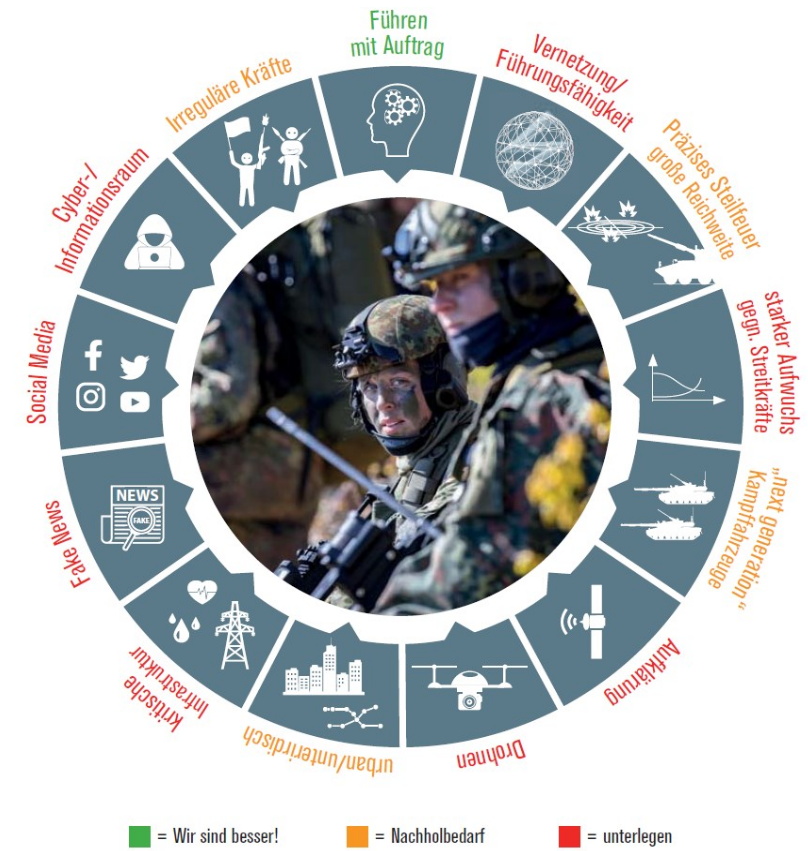
\includegraphics{images/mdo-bw.png} \emph{Grafik die den aktuellen
	Zustand erläutert}

\subsubsection{Fazit - JW als Königsdisziplin der modernen
	Kriegführung}\label{fazit---jw-als-kuxf6nigsdisziplin-der-modernen-kriegfuxfchrung}

\begin{itemize}
	\tightlist
	\item
	      Ab Airland Battle und dem spezifischen Akzent auf offensives Manöver
	      (statt Abnutzung) zur Paralysierung des Gegners wiederholt gefordert
	\item
	      Multidomain Operations (MDO) als neueste Konzeption der
	      wirkungsraumübergreifenden Kriegführung mit bislang unscharfen
	      Konturen
	\item
	      Wirksamkeit gegen Hauptbedrohung/-gegner bisher nur wenig erwiesen:
	      tönt einfach, schwierig in Umsetzung
	\item
	      Stark von amerikanischen Denkern und Technologiegläubigkeit geprägt
	\item
	      Franz-Stefan Gady: Jede Streitkraft praktiziert heute in irgendeiner
	      Weise diesen Kampf der verbundenen Waffen {[}\ldots{]} Ich nenne ihn
	      oft die militärische Königsdiziplin. Beherrscht man ihn, kann man die
	      eigenen Verluste niedrig halten und die des Gegner erhöhen.
\end{itemize}

\subsection{Geopolitik und
	Geostrategie}\label{geopolitik-und-geostrategie}

\subsubsection{Leitfragen}\label{leitfragen-1}

\begin{itemize}
	\tightlist
	\item
	      Wie hat sich die Geopolitik und -strategie als Denkschule etabliert?
	\item
	      Welche Vertreter haben sie in den letzten Jahren geprägt?
	\item
	      Welche Prämissen und Limitationen lassen sich aus dieser Denkschule
	      ableiten?
\end{itemize}

\begin{quote}
	{[}Geography is{]} the mother of strategy.\\
	- \emph{C.Gray and G.Sloan in Geopolitics, Geography and Strategy,
		London 1999}
\end{quote}

\subsubsection{Lektüre}\label{lektuxfcre-1}

\begin{itemize}
	\tightlist
	\item
	      Colin Flint, Introduction to Geopolitics, London 2022 S. 1-20.
	\item
	      Halford J. Mackinder, The Geographical Pivot of History, in: The
	      Geographical Journal, Vol. XXIII (4), 1904, S. 7-12.
\end{itemize}

\subsubsection{Heartland Theory}\label{heartland-theory}

Beginnt mit Rede von Halford J. Mackinder vor der Royal Geographic
Society, 25.01.1904: ``The Geographical Pivot of History''

\begin{itemize}
	\tightlist
	\item
	      Grundkonflikt: Seemächte gegen Landmächte

	      \begin{itemize}
		      \tightlist
		      \item
		            Vorteil für Landmächte, besonders jene mit Pivot Area = Heartland
		            wegen:
		      \item
		            Topographie / Geschichte
		      \item
		            Geographie-Ökonomie
		      \item
		            Technik / Eisenbahn
	      \end{itemize}
	\item
	      Politische Empfehlungen

	      \begin{itemize}
		      \tightlist
		      \item
		            1904: Gegenallianz der Seemächte
		      \item
		            1919: Pufferzone in Osteuropa
	      \end{itemize}
\end{itemize}

\begin{quote}
	Who rules East Europe commands the Heartland\\
	Who rules the Heartland commands the World-Island\\
	Who rules the World-Island commands the World.\\
	- \emph{Halford Mackinder, Democratic Ideals and Reality, New York 1919}
\end{quote}

\subsubsection{Rimland-Theorie}\label{rimland-theorie}

Beginnt mit Nicholas Spykman, America's Strategy in World Politics, New
York 1942

\begin{quote}
	Who controls the rimland rules Eurasia,\\
	Who rules Eurasia controls the destinies of the world.\\
	- \emph{The Geography of the Peace, New York 1944}
\end{quote}

\subsubsection{Game Plan und das Grand
	Chessboard}\label{game-plan-und-das-grand-chessboard}

Beginnt mit Zbigniew Brzezinski, Game Plan. A Geostrategic Framework for
the Conduct of the US-Soviet Contest, New York 1986

\begin{quote}
	Whoever controls Eurasia dominates the globe. If the Soviet Union
	captures the peripheries of this landmass {[}\ldots{]} it would not only
	win control of vast human,economic and military resources, but also gain
	access to the geostrategic approaches to the Western Hemisphere -- the
	Atlantic and the Pacific {[}\ldots{]}\\
	- \emph{A Geostrategic Framework for the Conduct of the US-Soviet
		Contest, New York 1986, S. 22-23:}
\end{quote}

\subsubsection{Kampf der Kulturen}\label{kampf-der-kulturen}

Beginnt mit Samuel Huntington, The Clash of Civilizations 1993 und The
Clash of Civilizations and the Remaking of World Order (1996)

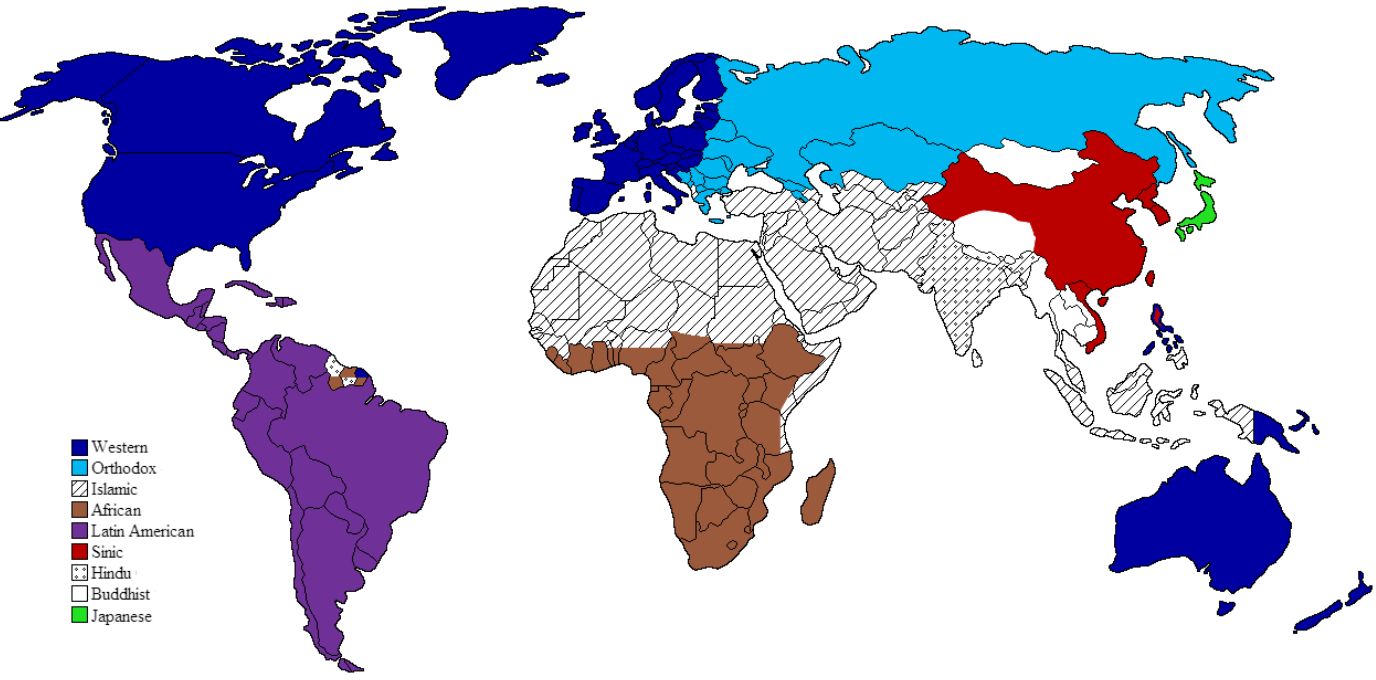
\includegraphics{images/huntington.png} \emph{Einteilung der Welt nach
	Kulturräumen}

\subsubsection{Geoökonomie und
	Friend-shoring}\label{geouxf6konomie-und-friend-shoring}

Fähigkeit von Regierungen, die wirtschaftliche Stärke ihrer Länder aus
bestehenden Finanz- und Handelsbeziehungen zu nutzen, um geopolitische
Lattice-like Security Architecture in Asien und wirtschaftliche Ziele zu
erreichen.

\subsubsection{Lattice-like Security Architecture in
	Asien}\label{lattice-like-security-architecture-in-asien}

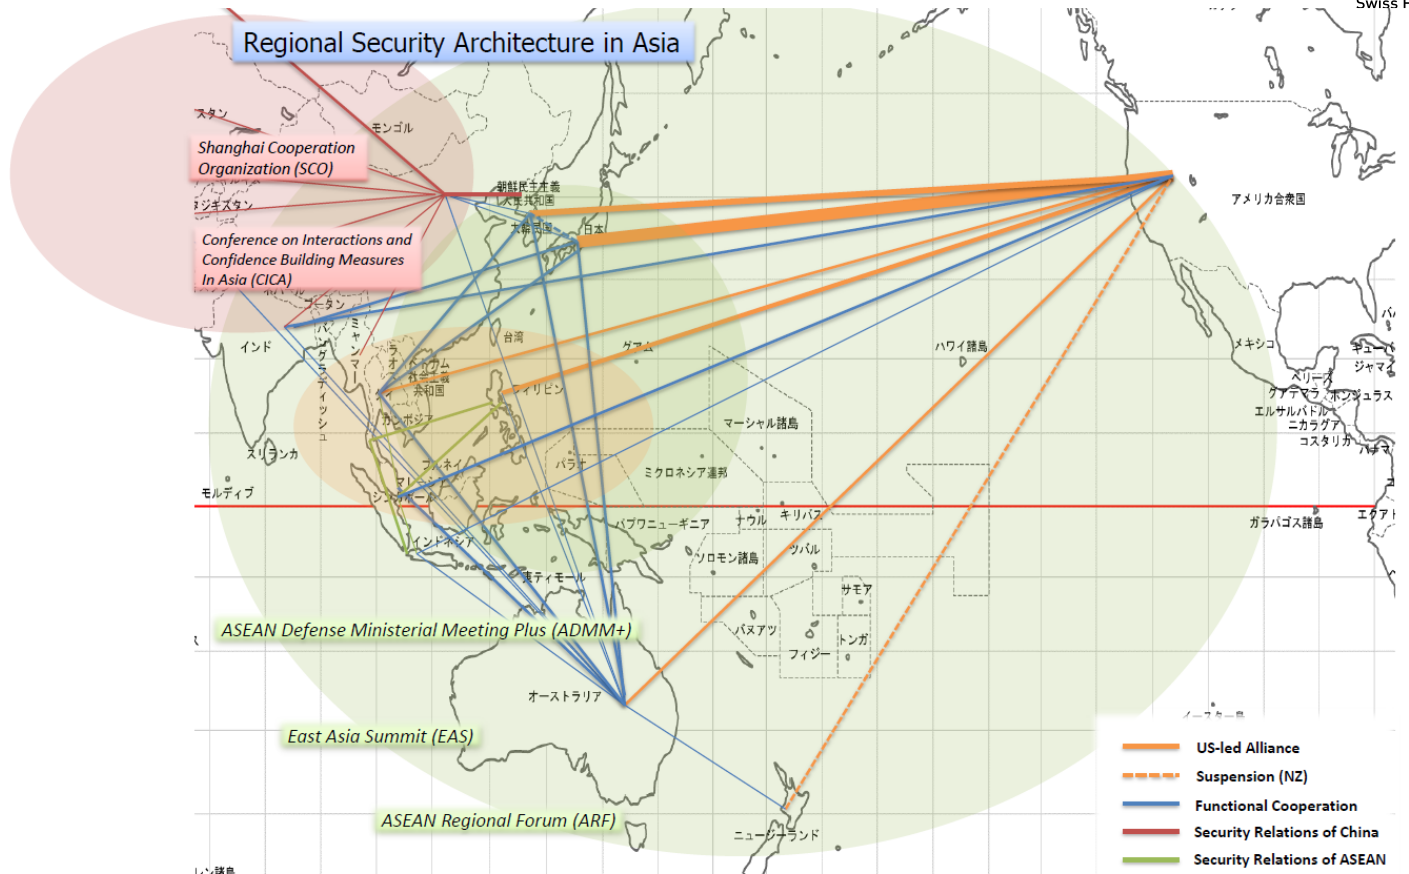
\includegraphics{images/lattice.png} \emph{Hub-and-Spokes Allianzsystem
	in Asien}

\subsubsection{Fazit}\label{fazit}

\begin{itemize}
	\tightlist
	\item
	      Eigenständige Theorieschule(n) mit Anspruch auf Erklärung der
	      Gegenwart und auf langfristige Prognosen
	\item
	      Hoher, interdisziplinärer Anspruch: Verbindung von (Aussen-)
	      Sicherheitspolitik mit Natur- und Geisteswissenschaften (Geografie,
	      Evolutionsbiologie, Geschichte \ldots)
	\item
	      Breitenwirkung
	\item
	      Überbewertung angeblicher ``Konstanten''
	\item
	      Unterschätzung der Irrationalität von Entscheidungsträgern und der
	      technologischen Entwicklung
	\item
	      Politischer Opportunismus,
	\item
	      Wissenschaftlichkeit fragwürdig
	\item
	      Eurasia is thus the chessboard on which the struggle for global
	      primacy continues to be played, and that struggle involves
	      geostrategy. Zbigniew Brzezinski, The Grand Chessboard: American
	      Primacy and Its Geostrategic Imperatives, New York 1997
\end{itemize}

\subsection{Sowjetische
	Militärstrategie}\label{sowjetische-milituxe4rstrategie}

\subsubsection{Leitfragen}\label{leitfragen-2}

\begin{itemize}
	\tightlist
	\item
	      Welche strategische Kultur galt für das sowjetische Militär?
	\item
	      Inwiefern fügt sich das Konzept der Tiefen Operation in die
	      sowjetische Militärstrategie ein?
	\item
	      Welche Elemente der sowjetische Militärstrategie wirken für die
	      aktuelle russische Militärstrategie nach?
\end{itemize}

\subsubsection{Lektüre}\label{lektuxfcre-2}

\begin{itemize}
	\tightlist
	\item
	      Hans-Ulrich Seidt, Alexander Swetschin und das strategische Denken
	      Russlands: Ein Beitrag zur Diskussion über Moskaus neue
	      Militärdoktrin, in: Osteuropa, Juli 1994, S. 630- 642.
\end{itemize}

\subsubsection{Kaiserlich Russische
	Armee}\label{kaiserlich-russische-armee}

Konzeptionsstreit im 18. und 19. Jahrhundert, Abnützung oder Zerstörung

\begin{itemize}
	\tightlist
	\item
	      Michail Kutusow (1745-1813): Russland gewinnt Kriege durch Geduld.
	\item
	      Alexander Suworow (1730- 1800): Russland gewinnt Kriege durch
	      Schnelligkeit.
\end{itemize}

\subsubsection{Michail Wassiljewitsch Frunse
	1885-1925}\label{michail-wassiljewitsch-frunse-1885-1925}

Zentrale Forderungen an sowjetische Militärstrategie:

\begin{itemize}
	\tightlist
	\item
	      Nächster Krieg langwierig und defensiv
	\item
	      Operationsraum wegen weitreichender Mittel riesig
	\item
	      Front und Hinterland organisatorisch vernetzen
	\item
	      Gesellschaft und Wirtschaft militarisieren
	\item
	      Wenn nötig, dann direkter Gewalteinsatz (kein indirekter Ansatz)
	\item
	      Ideologische Beeinflussung
\end{itemize}

\subsubsection{Rote Armee: Erneuter Konzeptionsstreit
	1928/29}\label{rote-armee-erneuter-konzeptionsstreit-192829}

\begin{itemize}
	\tightlist
	\item
	      Abnutzung: Alexander Swetschin 1978-1938
	\item
	      Zerstörung: Wladimir Triandafillow 1987-1931, Michail Tuchatschewski
	      1893-1937
\end{itemize}

\subsubsection{Alexander Swetschin und die Operative
	Stufe}\label{alexander-swetschin-und-die-operative-stufe}

\begin{itemize}
	\tightlist
	\item
	      Staat muss eine Übermobilisierung verhindern
	\item
	      Deshalb priorisiert Swetschin eine permanente Mobilisierung
	\item
	      Wirtschaftliches Hinterland muss sicher vor Krieg und Feind sein
	\item
	      Mischung aus Marxismus (Krieg als Fortsetzung der Politik) und
	      Maoismus (verschiedene Fronten in langem Krieg)
\end{itemize}

\paragraph{Theorie der Operativen
	Kunst}\label{theorie-der-operativen-kunst}

\begin{itemize}
	\tightlist
	\item
	      Drei militärische Stufen: Strategie, Operationskunst (neu), Taktik
	\item
	      Definition Operation modern, aber um Planung und Vorbereitung
	      erweitert
	\item
	      Forderung nach Vorbereitung und Durchführung durch Militärexperten
	\item
	      Organisation des Rückraums, um Operationen aufrecht zu halten
\end{itemize}

\subsubsection{Georgii Isserson und die Tiefe
	Operation}\label{georgii-isserson-und-die-tiefe-operation}

\begin{itemize}
	\tightlist
	\item
	      Von Anfang an offensive Vorgehensweise
	\item
	      Iteration Manöver -- Durchbruch durch Feuerkraft und Masse -- Manöver,
	      Vergleich mit Wellen
	\item
	      Folge: gestaffelte Aufstellung der Verbände, Phasierung
	\item
	      Riesiger Kräftebedarf
	\item
	      Unterstützung für Aufrüstungsprogramm Stalins
\end{itemize}

Mögliches Beispiel \textbf{Operation ``Bagration''}

\subsubsection{Blitzkrieg vs.~Tiefe
	Operation}\label{blitzkrieg-vs.-tiefe-operation}

\begin{longtable}[]{@{}
	>{\raggedright\arraybackslash}p{(\columnwidth - 4\tabcolsep) * \real{0.0495}}
	>{\raggedright\arraybackslash}p{(\columnwidth - 4\tabcolsep) * \real{0.4717}}
	>{\raggedright\arraybackslash}p{(\columnwidth - 4\tabcolsep) * \real{0.4788}}@{}}
	\toprule\noalign{}
	\begin{minipage}[b]{\linewidth}\raggedright
	\end{minipage} & \begin{minipage}[b]{\linewidth}\raggedright
		                 \textbf{Blitzkrieg}
	                 \end{minipage}            & \begin{minipage}[b]{\linewidth}\raggedright
		                                             \textbf{Tiefe Operation}
	                                             \end{minipage}                                  \\
	\midrule\noalign{}
	\endhead
	\bottomrule\noalign{}
	\endlastfoot
	\textbf{Bild}                               & 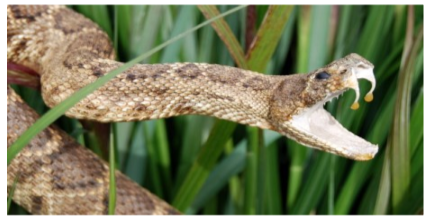
\includegraphics{images/gift.png}\emph{Giftschlange}   &
	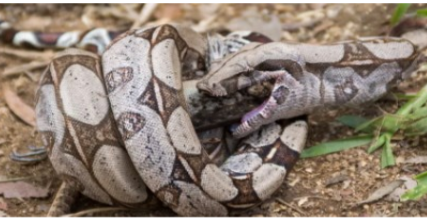
\includegraphics{images/druck.png}\emph{Würgeschlange}                                                                   \\
	\textbf{Durchbruch}                         & Schwerpunkt an einer Stelle, schmale
	Angriffsstreifen                            & Mehrere Stellen, breite Front                                              \\
	\textbf{Ziele}                              & Schwerpunkt an einer Stelle, schmale Angriffsstreifen,
	Sukzessive Einkesselung mit kleinen Einheiten, Erweiterung
	Durchbruchstelle, Vorrücken grosser Verbände, Einkesselung grosser
	Verbände, Aufrollen                         & Mehrere Stellen, breite Front, Wirkung
	gestaffelter Verbände in operative Tiefe, Ausfächern, Abschneiden,
	Aushungern, weniger Einkesselung von Zentren und Städte, Gegner in
	strategische Defensive zwingen                                                                                           \\
	\textbf{Manöver und Feuer}                  & Bewegung wichtiger als Feuer                           & Feuer
	wichtiger als Bewegung                                                                                                   \\
	\textbf{Akzentsetzung}                      & Qualität                                               & Quantität / Masse \\
	\textbf{Ausrichtung}                        & Offensiv                                               & Offensiv          \\
	\textbf{Rolle Luftwaffe}                    & Taktisch                                               & Operativ          \\
\end{longtable}

\subsubsection{Wassili Sokolowski und die Reformen der Tiefen
	Operation}\label{wassili-sokolowski-und-die-reformen-der-tiefen-operation}

Änderungen gegenüber Isserson / PU 36:

\begin{itemize}
	\tightlist
	\item
	      Operationsraum maximiert durch neue Waffen
	\item
	      Einsatz von Raketen à tous azimuts
	\item
	      Krieg muss in Initialphase entschieden werden
	\item
	      Konventionelle Streitkräfte zur Landesverteidigung und in regionalen
	      Kriegen
	\item
	      Bedeutungsverlust von Konzentration, Durchbruch, gestaffelte
	      Aufstellung
\end{itemize}

\subsubsection{Fazit: Sowjetische
	Militärstrategie}\label{fazit-sowjetische-milituxe4rstrategie}

\begin{itemize}
	\tightlist
	\item
	      Lange strategische Debatte in Russland: Abnützung oder Zerstörung?
	\item
	      Frunse weist auf Grösse und neue Mittel hin, seine Lösung besteht in
	      einer Militarisierung der Zivilgesellschaft und einer Vernetzung von
	      Front und Hinterland.
	\item
	      (Erneuter) Richtungsstreit in Roter Armee: Abnützung oder Zerstörung?
	\item
	      Swetschin priorisiert die Ermattung: Geduld und Abnützung des Gegners.
	\item
	      Swetschin führt die politikfreie operative Kunst ein: primär defensiv
	      ausgerichtet, Ziel: Gn ausmanövrieren.
	\item
	      Isserson sucht dagegen die Entscheidungsschlachten und erweitert die
	      schon unter Triandafillow entwickelte Offensivdoktrin der Tiefen
	      Operation.
	\item
	      Die Tiefe Operation benötigt einen gigantischen Kräftebedarf sowie
	      eine zentrale Planung und Steuerung.
	\item
	      Sokolowski erweitert die Tiefe Operation qualitativ und geographisch,
	      um im Kalten Krieg als strategische Abschreckung gegenüber der USA zu
	      dienen.
\end{itemize}

\subsection{Reguläre vs.~irreguläre
	Kriegführung}\label{reguluxe4re-vs.-irreguluxe4re-kriegfuxfchrung}

\subsubsection{Leitfragen}\label{leitfragen-3}

\begin{itemize}
	\tightlist
	\item
	      Wie hat sich die Unterscheidung zwischen regulärer und irregulärer
	      Kriegführung entwickelt?
	\item
	      Inwiefern unterscheidet das heutige Völkerrecht zwischen regulären und
	      irregulären Kombattanten?
	\item
	      Was besagt das Paradigma der neuen Kriege?
\end{itemize}

\begin{quote}
	You know you never defeated us on the battlefield,' said the American
	colonel. The North Vietnamese colonel pondered this remark a moment.
	`That may be so,' he replied, 'but it is also irrelevant.\\
	- \_Conversation in Hanoi, April 1975, zit. n.~Harry G. Summers\_\_
\end{quote}

\subsubsection{Lektüre}\label{lektuxfcre-3}

\begin{itemize}
	\tightlist
	\item
	      Colin S. Gray, Irregular Warfare: One Nature, Many Characters, in:
	      Strategic Studies Quarterly, Vol. 1 (2), 2007), S. 35-57.
\end{itemize}

\subsubsection{Krieg im Völkerrecht: Ius ad bellum vs.~ius in
	bello}\label{krieg-im-vuxf6lkerrecht-ius-ad-bellum-vs.-ius-in-bello}

\begin{itemize}
	\tightlist
	\item
	      Ius ad bellum: Das Recht zum Krieg

	      \begin{itemize}
		      \tightlist
		      \item
		            Mit dem Kriegsverbot von 1945 soll die Clausewitz'sche Losung, Der
		            Krieg ist eine blosse Fortsetzung der Politik mit anderen Mitteln,
		            aufgegeben werden.
	      \end{itemize}
	\item
	      Ius in bello: Das Recht im Krieg

	      \begin{itemize}
		      \tightlist
		      \item
		            Humanitäres Völkerrecht oder Kriegsrecht regelt, was im Krieg
		            zulässig ist.
	      \end{itemize}
\end{itemize}

\subsubsection{Regulärer Kombattant}\label{reguluxe4rer-kombattant}

Die Gesetze, die Rechte und die Pflichten sondern auch für die Milizen
und Freiwilligen-Korps, wenn sie die folgenden Bedingungen in sich
vereinigen:

\begin{enumerate}
	\def\labelenumi{\arabic{enumi}.}
	\tightlist
	\item
	      dass jemand an ihrer Spitze steht, der für seine Untergebenen
	      verantwortlich ist,
	\item
	      dass sie ein bestimmtes, aus der Ferne, erkennbares Abzeichen tragen,
	\item
	      dass sie die Waffen offen führen und
	\item
	      dass sie bei ihren Unternehmungen die Gesetze und Gebräuche des
	      Krieges beobachten.
\end{enumerate}

\subsubsection{Irregulärer Kombattant}\label{irreguluxe4rer-kombattant}

\begin{enumerate}
	\def\labelenumi{\arabic{enumi}.}
	\tightlist
	\item
	      Ist Teil einer politisch nicht rechenschaftspflichtigen Organisation
	\item
	      ist äusserlich nicht von der Zivilbevölkerung unterscheidbar
	\item
	      trägt Waffen nicht offen
	\item
	      missachtet das Kriegsvölkerrecht
\end{enumerate}

\subsubsection{Akademische
	Datensammlung}\label{akademische-datensammlung}

\begin{itemize}
	\tightlist
	\item
	      Uppsala Conflict Data Programm UCDP
	\item
	      Our World in Data OWID
\end{itemize}

\subsubsection{Debatte um die ``neuen
	Kriege''}\label{debatte-um-die-neuen-kriege}

Mary Kaldor, New and Old Wars. Organised Violence in a Global Era,
Cambridge 2012 (3. Auflage)

\begin{itemize}
	\tightlist
	\item
	      Seit dem Ende des 20. Jahrhunderts gibt es einen neuen Kriegstypus:
	      der neue Krieg
	\item
	      Darin verschmelzen Krieg, organisierte Kriminalität und kollektive
	      Menschen- rechtsverletzungen
	\item
	      Neue Kriege sind privatisiert und informell
	\item
	      Globalisierung, Technologie und transna- tionaler Austausch in den
	      Bereichen Politik, Ökonomie, Militär und Kultur fördern Neue Kriege
	\item
	      Soziale (nicht technologische) Revolution in military affairs
	\item
	      Staatliches Gewaltmonopol für Kriege erodiert
	\item
	      Ziel der neuen Kriege liegt in Identitätspoli- tik, nicht länger
	      geopolitische oder ideolo- gische Ziele
	\item
	      Fear and hatred, statt hearts and minds
\end{itemize}

\subsubsection{Begriffsdefinition}\label{begriffsdefinition}

\begin{itemize}
	\tightlist
	\item
	      \textbf{Krieg} Anwendung organisierter bewaffneter Gewalt zwischen
	      menschlichen Kollektiven zur Durchsetzung von Interessen und mit Folge
	      von Todesopfern und physischen Schäden
	\item
	      \textbf{Regulärer Krieg} meint den Krieg zwischen zwei (oder mehr)
	      Staaten.
	\item
	      \textbf{Irregulärer Krieg} meint den Krieg zwischen einem (oder
	      mehreren) Staaten einerseits und einer (oder mehrerer)
	      nicht-staatlicher Gruppierungen andererseits.
\end{itemize}

\subsubsection{Spezialfall hybrider Krieg, hybride
	Bedrohung}\label{spezialfall-hybrider-krieg-hybride-bedrohung}

\begin{quote}
	Hybrid wars incorporate a range of different modes of warfare, including
	conventional capabilities, irregular tactics and formations, terrorist
	acts including indiscriminate violence and coercion, and criminal
	disorder.\\
	- \emph{Frank G. Hoffman, Conflict in the 21st Century: the Rise of
		Hybrid Wars, Arlington 2007}
\end{quote}

\begin{quote}
	I define a hybrid threat as: Any adversary that simultaneously and
	adaptively employs a fused mix of conventional weapons, irregular
	tactics, terrorism and criminal behavior in the battle space to obtain
	their political objectives.\\
	- \emph{Frank G. Hoffman, Hybrid vs.~Compound War, Armed Forces}
\end{quote}

\subsubsection{Fazit}\label{fazit-1}

\begin{itemize}
	\tightlist
	\item
	      Der Krieg ist völkerrechtlich geächtet. Das moderne Völkerrecht
	      spricht nur noch von bewaffnetem Konflikt.
	\item
	      Krieg ist nur noch ein politischer Begriff und als solcher nicht
	      normiert; alle Abgrenzungen zum Nicht-Krieg sind willkürlich. Auch das
	      allgemeine Verständnis hat unscharfe Konturen.
	\item
	      Krieg ist ein hochkomplexes, dynamisches Phänomen, dass sich nicht mit
	      einfachen Formeln (alt/neu, (un)konventionell, (a)symmetrisch,
	      (ir)regulär, hybrid etc.) kategorisieren lässt.
	\item
	      Regulärer Krieg meint den Krieg zwischen
	\item
	      Wir unterscheiden einzig zwischen regulärem/irregulärem Krieg.
	\item
	      Im Krieg dominiert die Asymmetrie, auch weil sie von den
	      Kriegsparteien aktiv angestrebt wird. Symmetrien sind allenfalls
	      punktuell und temporär
\end{itemize}

\subsection{Aufstandstheorien}\label{aufstandstheorien}

\subsubsection{Leitfragen}\label{leitfragen-4}

\begin{itemize}
	\tightlist
	\item
	      Welche strategischen Grundsätze verfolgen irreguläre Kämpfer?
	\item
	      Weshalb waren gewisse Aufstandsbewegungen erfolgreich?
	\item
	      Welche Rolle spielt die Zivilbevölkerung während Aufständen?
\end{itemize}

\subsubsection{Lektüre}\label{lektuxfcre-4}

\begin{itemize}
	\tightlist
	\item
	      Seth G. Jones/Patrick B. Johnston, The Future of Insurgency, in:
	      Studies in Conflict \& Terrorism, Vol. 36 (1), 2013, S. 1-25.
\end{itemize}

\subsubsection{Aufstand als Konstante der
	Strategiegeschichte}\label{aufstand-als-konstante-der-strategiegeschichte}

\begin{itemize}
	\tightlist
	\item
	      Amerikanischer Unabhängigkeitskrieg
	\item
	      Guerilla in Spanien
	\item
	      Clausewitz (Vom Kriege, 6. Buch, 26. Kapitel, Volksbewaffnung)

	      \begin{itemize}
		      \tightlist
		      \item
		            dass der Krieg im Innern des Landes geführt
		      \item
		            dass er nicht durch eine einzige Katastrophe entschieden werde
		      \item
		            dass das Kriegstheater eine beträchtliche Länderstrecke einnehme
		      \item
		            dass der Volkscharakter die Massregel unterstütze
		      \item
		            dass das Land sehr durchschnitten und unzugänglich sei, entweder
		            durch Gebirge oder durch Wälder und Sümpfe oder durch die Natur der
		            Bodenkultur
	      \end{itemize}
\end{itemize}

\subsubsection{Generelle
	Aufstandsstrategie}\label{generelle-aufstandsstrategie}

\begin{itemize}
	\tightlist
	\item
	      Keine Suche nach Entscheidungsschlacht, stattdessen Überdehnung Gegner
	\item
	      Hohe Kosten für Gegner (materiell, aber auch politische Legitimität)
	      provozieren
	\item
	      Unterstützung durch Bevölkerung entscheidend (aktive Minderheit und
	      passive Mehrheit)
	\item
	      Schrittweiser Übergang zu direkterer Konfrontation mit Gegner mit
	      zunehmender Macht und Gebietskontrolle
\end{itemize}

\subsubsection{Kategorien des Aufstands}\label{kategorien-des-aufstands}

\begin{longtable}[]{@{}
	>{\raggedright\arraybackslash}p{(\columnwidth - 6\tabcolsep) * \real{0.1520}}
	>{\raggedright\arraybackslash}p{(\columnwidth - 6\tabcolsep) * \real{0.2573}}
	>{\raggedright\arraybackslash}p{(\columnwidth - 6\tabcolsep) * \real{0.2827}}
	>{\raggedright\arraybackslash}p{(\columnwidth - 6\tabcolsep) * \real{0.3080}}@{}}
	\toprule\noalign{}
	\begin{minipage}[b]{\linewidth}\raggedright
	\end{minipage}                     & \begin{minipage}[b]{\linewidth}\raggedright
		                                     ethnisch-nationalistisch motivierter Aufstand
	                                     \end{minipage}                   & \begin{minipage}[b]{\linewidth}\raggedright
		                                                                        sozialrevolutionärer Aufstand
	                                                                        \end{minipage} & \begin{minipage}[b]{\linewidth}\raggedright
		                                                                                         Islamistischer ``Aufstand''
	                                                                                         \end{minipage}                                        \\
	\midrule\noalign{}
	\endhead
	\bottomrule\noalign{}
	\endlastfoot
	Selbstbezeichnung der Insurgenten                               & Guerillero, Partisan, Résistance-
	bzw. Freiheitskämpfer                                           & Revolutionär, Guerillero                                        & Mudschahid
	(``Gotteskrieger'')                                                                                                                                                        \\
	Strategisches Ziel bzw. politische Legitimation der Insurgenten &
	Abschütteln Fremdherrschaft, Machtübernahme (daher Aufbau regulärer
	Streitkräfte)                                                   & Sturz ``ungerechte'', reaktionäre Herrschaft,
	Machtübernahme (daher Aufbau reg. Streitkräfte)                 & Zurückdrängung west.
	Einfluss in islamischer Welt, Sturz säkularer Regimes, islamische
	Herrschaft (lokal/regional bis global (AQ, IS))                                                                                                                            \\
	Taktisch-operative Primär-Ziele der Insurgenten                 & Gegnerische
	Sicherheitskräfte: Beeinflussung Kosten-Nutzen-Rechnung des Gegners,
	Ermattung Gegner. Anfänglich defensive Kriegführung             & Gegnerische
	Sicherheitskräfte: Zerschlagung gegnerisches Potenzial (in Raten).
	Anfänglich defensive Kriegführung                               & Gegnerische Sicherheitskräfte,
	Zivilbevölkerung                                                                                                                                                           \\
	``Exit-Option'' für den Gegner?                                 & Ja (Exil, Rückzug)                                              & Nein (da
	``Volksfeind'')                                                 & Unterschiedlich (nicht für Juden)                                                                        \\
	Rekrutierung und Finanzierung, operative Steuerung              & national, zentral                                               &
	transnational-global, zentral                                   & transnational-global, dezentral                                                                          \\
	Adressat der Insurgenten (der über Mediatisierung ``zu interessierende
	Dritte'')                                                       & eigene Nation                                                   & Bürger (``tier état''), internationale
	Arbeiterklasse (``Proletariat'')                                & Islamische Gemeinschaft
	(``Ummah'')                                                                                                                                                                \\
	Mittel                                                          & Nutzung eigener Zivilbevölkerung als logistische Basis, Bündnis
	mit ausländischer Armee möglich                                 & Nutzung der Infrastruktur des Gegners,
	Bündnis mit ausl. Armee möglich                                 & Nutzung der Infrastruktur des Gegners,
	eigene Bevölkerung, Kooperation/Allianzen möglich                                                                                                                          \\
	Waffeneinsatz                                                   & konventionell, beschränkt (low tech)                            & konventionell,
	beschränkt (low tech)                                           & konv. (low tech -- high tech (Hisbollah), ABC
	(angestrebt)                                                                                                                                                               \\
	Hauptschauplätze                                                & Spanischer Aufstand gegen Napoleon (1807- 14),
	Aufstände in Kolonien (ab 1914), Widerstand (1940-45), Indochina/Vietnam
	(1963-73)                                                       & Franz. Revolution (1789), Liberale Rev.~in Deutschland
	(1848/49), Pariser Kommune (1871), chines. Bürgerkrieg (1928-36, 1945-
	49), Kuba (1956-58)                                             & Afghanistan, Libanon (ab 1980er Jahre),
	Israel/PA-Gebiete (ab 1988); Algerien (ab 1990er Jahre), Irak, Syrien,
	Jemen, Somalia, Nigeria, Mali, Südostasien usw.                                                                                                                            \\
	Theoretische Grundlagen (z.B.)                                  & T.E. Lawrence (of Arabia), Giap, von
	Dach                                                            & Engels, Lenin, Trotzki, Mao Tse-tung, Che Guevara, Marighella,
	Giap                                                            & Qutb, Fadlallah, Azzam, al-Suri, Naji                                                                    \\
\end{longtable}

\subsubsection{Aufstandsmodelle}\label{aufstandsmodelle}

\paragraph{Maoistisches Modell}\label{maoistisches-modell}

\begin{itemize}
	\tightlist
	\item
	      Phase I: Klandestine Agitation, Propaganda, Indoktrinierung
	\item
	      Phase II: Expansion durch irreguläre Kriegführung
	\item
	      Phase III: Zerstörung durch konventionelle Konfrontation
\end{itemize}

\paragraph{Foco}\label{foco}

\begin{itemize}
	\tightlist
	\item
	      Durchführung militärischer Aktionen durch Avantgarde (Foco)
	\item
	      Zustrom durch Landbevölkerung
	\item
	      Sukzessive Ausdehnung durch neue Focos
\end{itemize}

\paragraph{Algerische Front de Libération Nationale
	(FLN)}\label{algerische-front-de-libuxe9ration-nationale-fln}

\begin{itemize}
	\tightlist
	\item
	      Maostisches Modell in Kombination mit Terrorismus im urbanen Raum
	\item
	      Überreaktion der Sicherheitskräfte
	\item
	      führt zu Unterminierung Aufstandsbekämpfung
\end{itemize}

\paragraph{Provisional Irish Republican Army
	(PIRA)}\label{provisional-irish-republican-army-pira}

\begin{itemize}
	\tightlist
	\item
	      Simultane Nutzung von Gewaltanwendung, zivilem Ungehorsam (Streiks,
	      Demonstrationen, Sitzblockaden, Hungerstreiks), politische
	      Partizipation
\end{itemize}

\subsubsection{Friedrich Engels
	1820-1895}\label{friedrich-engels-1820-1895}

\paragraph{Der Aufstand als Kunst
	1852}\label{der-aufstand-als-kunst-1852}

\begin{itemize}
	\tightlist
	\item
	      Ausgleich Nachteile (Organisation, Disziplin, Autorität) vor Eröffnung
	      des Kampfes
	\item
	      Entschlossenheit bei Eröffnung des Kampfes
	\item
	      Nachhaltige offensive Kampfführung (Momentum)
	\item
	      Gewinnung Unentschlossener
\end{itemize}

\paragraph{Die Kriegsführung des Proletariats
	1852}\label{die-kriegsfuxfchrung-des-proletariats-1852}

\begin{itemize}
	\tightlist
	\item
	      Neue Kriegsmethode: Emanzipiertes Proletariat nutzt
	      (militär-)technische Errungenschaften
	\item
	      Revolutionäre Truppe wird in konventionelle Massenarmee umgewandelt
\end{itemize}

\subsubsection{Mao Tse-tung 1893-1976}\label{mao-tse-tung-1893-1976}

\paragraph{Ein Funke kann die ganze Steppe in Brand setzen
	1930}\label{ein-funke-kann-die-ganze-steppe-in-brand-setzen-1930}

\begin{itemize}
	\tightlist
	\item
	      Elastizität (Konzentration, Dispersion)
	\item
	      ``Kreiseziehen'': Agitation in der Bevölkerung
\end{itemize}

\paragraph{Guerrilla Warfare 1937}\label{guerrilla-warfare-1937}

\begin{itemize}
	\tightlist
	\item
	      subsidiär in langem Krieg (Feind technisch überlegen, aber ausgedünnt)
	\item
	      Selbsterhaltung (= Grund-Axiom) und Wachstum
	\item
	      Elastizität (s.o.), Offensive/Defensive/Verzögerung
	\item
	      Basen/Operationen im feindbesetzten Gebiet (äussere Linien)
\end{itemize}

\paragraph{Militärischen Prinzipien zum Sieg über Chiang Kai-shek
	1947}\label{milituxe4rischen-prinzipien-zum-sieg-uxfcber-chiang-kai-shek-1947}

\begin{itemize}
	\tightlist
	\item
	      Konzentration (Schaffung punktueller Überlegenheit) gegen
	      Opportunitätsziele, Vernichtung
	\item
	      Dispersion gegenüber feindlicher Überlegenheit
	\item
	      Wachstum durch Überläufer, Stärkung durch Beute
\end{itemize}

Voraussetzungen: Vorbereitung, Mut, Opfersinn, Ausdauer, Beweglichkeit,
Erholung.

\subsubsection{Hans von Dach 1926-2002}\label{hans-von-dach-1926-2002}

Der totale Widerstand: Kleinkriegsanleitung für jedermann, Bern 1957

\begin{itemize}
	\tightlist
	\item
	      Grundszenario: CH Nebenschauplatz von Gegner, dessen Kräfte an vielen
	      Fronten gebunden, CH-Volksaufstand Teil breiterer Erhebung.
	\item
	      Volksaufstand: unvermeidlich, machbar, legitim/moralisch/ehrenvoll,
	      stärkt Verhandlungsposition in Nachkriegszeit.
	\item
	      Widerstandsorganisation: Beitrag zur Kriegsverhinderung
	      (Abschreckung), Verlängerung des Krieges, Schädigung des Besatzers,
	      Fernziel: allgemeiner offener Aufstand.
	\item
	      Beziehung zur regulären Armee: ``Auffangorganisation'' für versprengte
	      Kader/Mannschaften und Milizorganisationen, Anknüpfung an
	      Grundausbildung Armee und Taktiken Jagdkampf, Ergänzung um technische
	      und taktische Anleitung für Kleinkrieg.
\end{itemize}

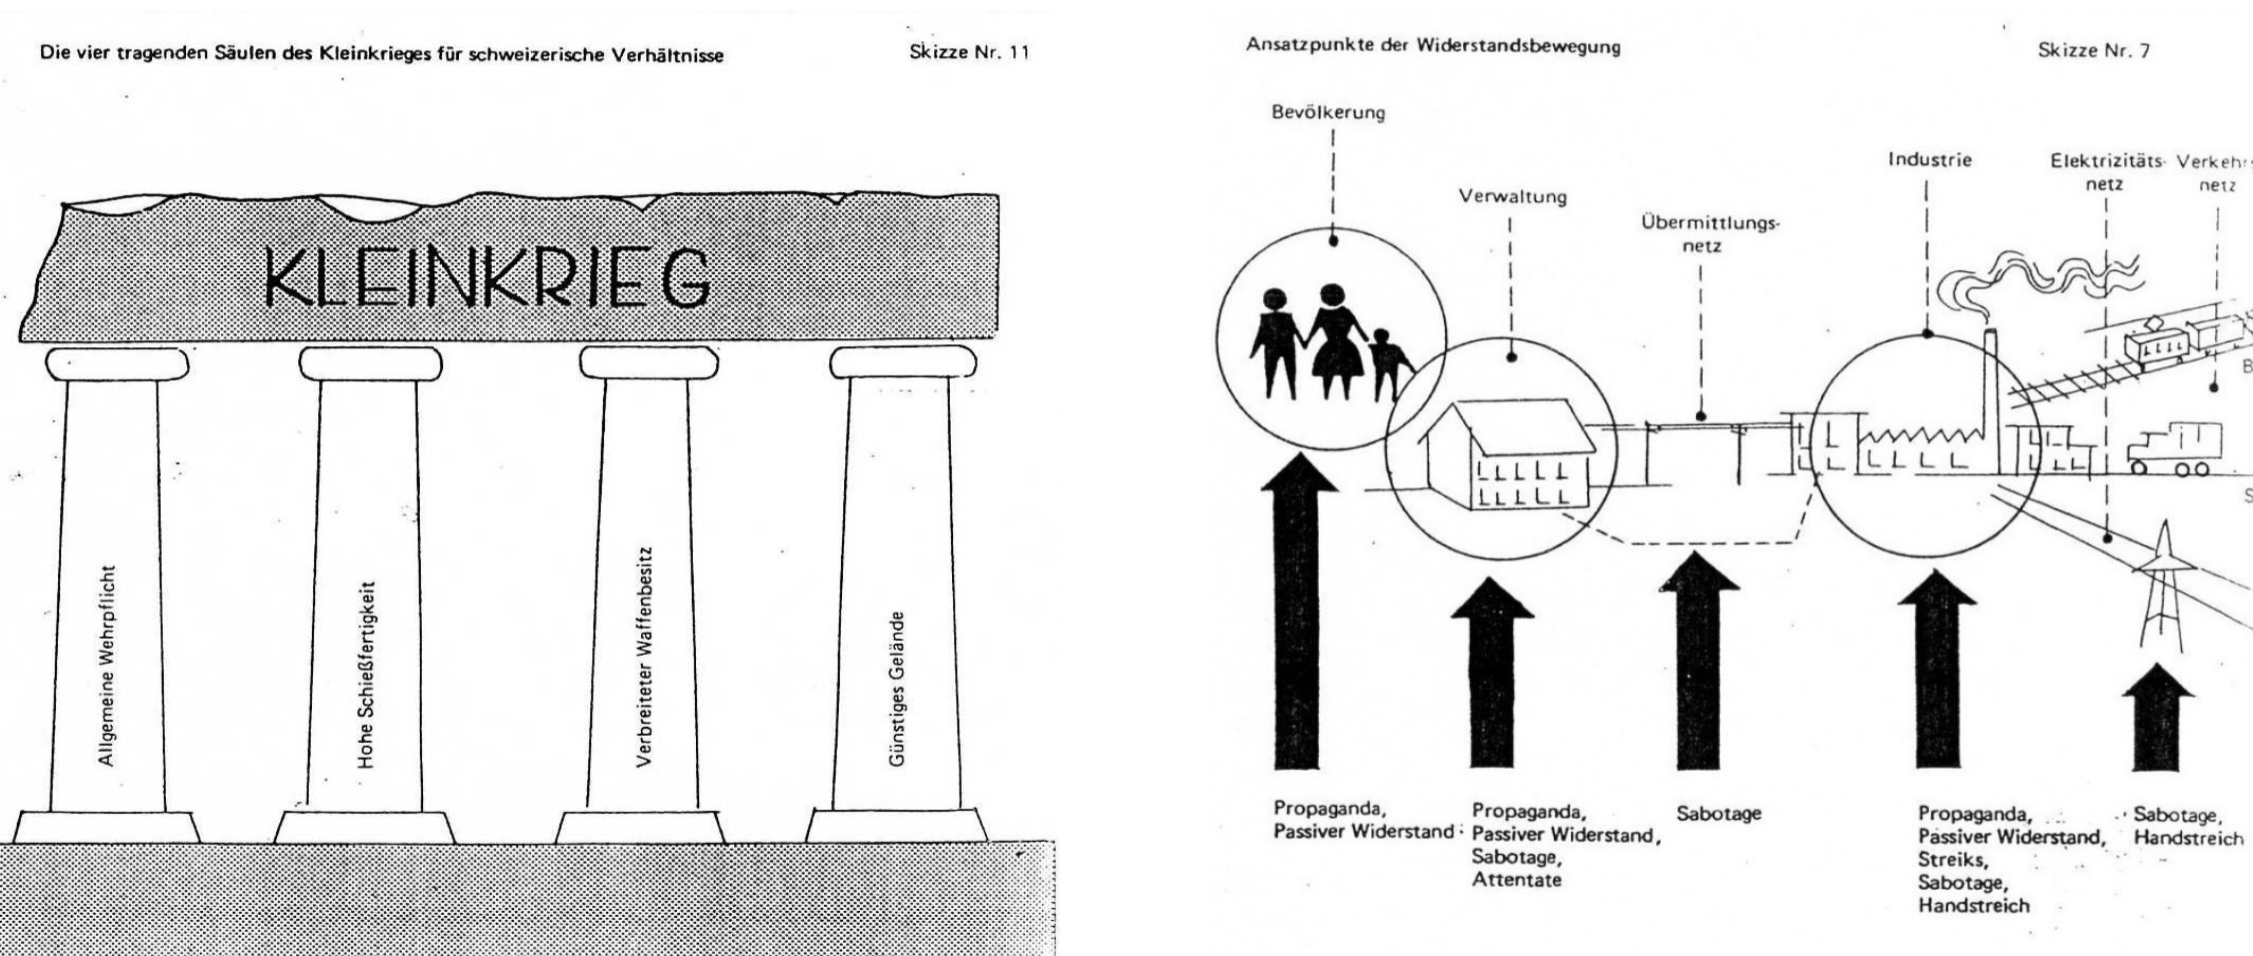
\includegraphics{images/hans.png} \emph{Skizzen zur
	Kleinkriegsanleitung}

\subsubsection{Ernesto (Che) Guevara
	(1928-1967)}\label{ernesto-che-guevara-1928-1967}

Beginn, Entwicklung und Ende des Guerillakrieges, Berlin 1968

\begin{itemize}
	\tightlist
	\item
	      Etappe 1: Bestehen einer (isolierten) Avantgarde (= ``Foco'')
	\item
	      Etappe 2: Einzeloperationen des Foco: Zustrom von Landbewohnern;
	      grössere Bewegungsfreiheit
	\item
	      Etappe 3: Provisorische werden zu festen Einrichtungen,
	      Guerilla-Industrie
	\item
	      Etappe 4: Erbeutung von Waffen, (Proto-)Regierung/Verwaltung, Gesetze,
	      Schulung/Propaganda
	\item
	      Etappe 5: Weitere Foco-Ableger bis in Vorstädte
	\item
	      Etappe 6: Sabotage, Terror in ``ungünstigen'' (= städtischen) Gebieten
	\item
	      Etappe 7: Guerilla mutiert zu regulärer Armee: Gegner kapituliert
\end{itemize}

Kontinuierliche Ausweitung der Operationsraums durch Bildung immer neuer
``Focos'' und Verschmelzung mit dem Volk.

\subsubsection{Suizidattentat: Innovation und
	Wissensdiffusion}\label{suizidattentat-innovation-und-wissensdiffusion}

\begin{itemize}
	\tightlist
	\item
	      Erste, gezielte Anwendungen durch Hisbollah zu Beginn 1980er Jahre
	\item
	      Verbreitung durch Inspiration/Imitation oder Kooperation/Ausbildung
	\item
	      Spektrum: linksnationalistische -- radikalislamistische Gruppierungen;
	      grösster Anteil: Globale Dschihad-Bewegung
\end{itemize}

\subsubsection{Externe Unterstützung als potenzieller
	Erfolgsfaktor}\label{externe-unterstuxfctzung-als-potenzieller-erfolgsfaktor}

\begin{itemize}
	\tightlist
	\item
	      Formen externer Unterstützung

	      \begin{itemize}
		      \tightlist
		      \item
		            Sicherer Zufluchtsort
		      \item
		            Finanzielle Mittel und Kriegsmaterial
		      \item
		            Ausbildung
		      \item
		            ND-Erkenntnisse, Planung von Operationen
		      \item
		            Unterstützendes Feuer
	      \end{itemize}
	\item
	      Verbesserte militärische Fähigkeiten, Ressourcenzuwachs, politische
	      Anerkennung auf internationaler Ebene
	\item
	      Grosser Nutzen, aber auch potenziell signifikante Kosten und Risiken
\end{itemize}

\subsubsection{Fazit}\label{fazit-2}

\begin{itemize}
	\tightlist
	\item
	      Keine direkte Konfrontation mit militärisch überlegenem Gegner,
	      stattdessen Überdehnung und Kampf um politische Kontrolle und
	      Legitimität
	\item
	      Kombination von politischer Subversion und militärischen Aktionen,
	      zunehmende Gebietskontrolle erlaubt Ausbau militärischer Fähigkeiten
	      sowie Macht und Einfluss durch de-facto Regierung
\end{itemize}

\begin{enumerate}
	\def\labelenumi{\arabic{enumi}.}
	\tightlist
	\item
	      Sozialrevolutionärer Aufstand als zentrale Referenz für
	      sozialistischen Klassenkampf (bis Ende Kalter Krieg): Engels für
	      Revolutionen in (industrialisiertem) Europa; Mao und Che für
	      Revolutionen in (agrarischer) südlicher Hemisphäre
\end{enumerate}

\begin{itemize}
	\tightlist
	\item
	      Engels: Organisation, Entschlossenheit, Momentum
	\item
	      Mao: Drei Phasen des Volkskrieges, seriell:

	      \begin{itemize}
		      \tightlist
		      \item
		            Defensive: Aufbau Organisation, Rekrutierung
		      \item
		            Gleichgewicht: begrenzte Angriffe aus sicherem Gebiet
		      \item
		            Offensive: mit disziplinierter, regulärer Armee
		      \item
		            Kampf primär politisch (Analyse Beziehung Partisanen-Volk)
	      \end{itemize}
	\item
	      Che: Gewalt durch Avantgarde transformiert politische Situation,
	      Proliferation von Focos
\end{itemize}

\begin{enumerate}
	\def\labelenumi{\arabic{enumi}.}
	\setcounter{enumi}{1}
	\tightlist
	\item
	      Ethnisch-nationalistischer Aufstand
\end{enumerate}

\begin{itemize}
	\tightlist
	\item
	      von Dach: Umfassender Aufstandstheorie Rückgriff auf Besonderheiten
	      der Schweiz Idealisierung der Opferbereitschaft Unterschätzung
	      Risiken/Missbrauchspotenzial
\end{itemize}

\begin{enumerate}
	\def\labelenumi{\arabic{enumi}.}
	\setcounter{enumi}{2}
	\tightlist
	\item
	      Islamistischer Aufstand: Suizidattentat und Terrorismus
\end{enumerate}

\begin{itemize}
	\tightlist
	\item
	      Problem: Diskrepanz Theorie (Propaganda) -- Realität (Umsetzung)
\end{itemize}

\subsection{Aufstandsbekämpfungstheorien}\label{aufstandsbekuxe4mpfungstheorien}

\subsubsection{Leitfragen}\label{leitfragen-5}

\begin{itemize}
	\tightlist
	\item
	      Welche strategischen Grundsätze verfolgen organisierte Streitkräfte
	      bei der Bekämpfung von Aufständischen?
	\item
	      Weshalb waren gewisse reguläre Armeen erfolgreich in der
	      Niederschlagung von Aufständen?
	\item
	      Welche Rolle spielt die Zivilbevölkerung?
\end{itemize}

\subsubsection{Lektüre}\label{lektuxfcre-5}

\begin{itemize}
	\tightlist
	\item
	      David H. Petraeus, Learning Counterinsurgency: Observations from
	      Soldiering in Iraq, in: Military Review, January-February 2006, S.
	      45-55.
	\item
	      Gian P. Gentile, A Requiem for American Counterinsurgency, in: Orbis,
	      Vol. 57 (4), 2013, S. 549-558.
\end{itemize}

\subsubsection{Grundkonstellation
	Aufstandsbekämpfung}\label{grundkonstellation-aufstandsbekuxe4mpfung}

\begin{itemize}
	\tightlist
	\item
	      Lokale Aufständische vs.~externe Besatzungsmacht
	\item
	      Aufständische kämpfen zumeist irregulär und zwingen damit die
	      Besatzungsmacht in langwierige Pazifizierungs- und
	      Stabilisierungsoperationen fernab der Heimat
	\item
	      Aus der Perspektive der Besatzungsmächte wird deshalb von ``kleinen''
	      Kriegen (small wars, petites guerres) mit niedriger Intensität
	      gesprochen.
	\item
	      Die Aufstandsbekämpfungstheorien versuchen, eine Doktrin zum Sieg in
	      irregulären Kriegen zu formulieren
	\item
	      Simplifizierendes Kontinuum: population centric approach
	      \textless---\textgreater{} kinetic approach
\end{itemize}

\begin{quote}
	Comprehensive civilian and military efforts designed to simultaneously
	defeat and contain insurgency and address its root causes.\\
	- Definition COIN nach JP 1-02, S. 53
\end{quote}

\subsubsection{Aufstandsbekämpfung mit harter
	Hand}\label{aufstandsbekuxe4mpfung-mit-harter-hand}

\begin{itemize}
	\tightlist
	\item
	      Charles E. Callwell 1859-1928

	      \begin{itemize}
		      \tightlist
		      \item
		            Lessons to Be Learned from the Campaigns in Which British Forces
		            Have Been Employed, 1887
		      \item
		            Small Wars: Their Principles and Practice, 1896-1906
	      \end{itemize}
\end{itemize}

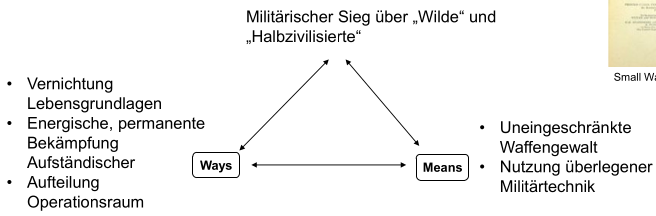
\includegraphics{images/callwell.png} \emph{Schematische Einordnung von
	Callwells Ansatz}

\subsubsection{Imperial Policing}\label{imperial-policing}

\begin{itemize}
	\tightlist
	\item
	      Charles W.Gwynn 1870-1962

	      \begin{itemize}
		      \tightlist
		      \item
		            Imperial Policing 1934
	      \end{itemize}
\end{itemize}

\begin{figure}
	\centering
	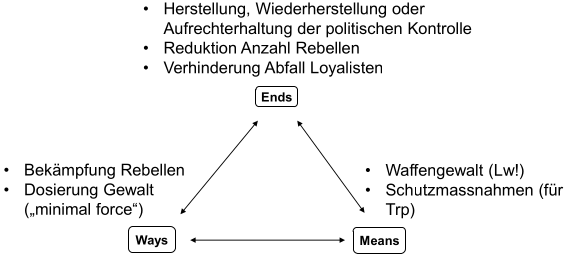
\includegraphics{images/gwynn.png}
	\caption{gwynn}
\end{figure}

\subsubsection{Malayan Emergency
	(1948-1960)}\label{malayan-emergency-1948-1960}

\begin{itemize}
	\tightlist
	\item
	      Emergency Regulations 1948, Briggs-Plan 1950
	\item
	      Umsiedlungen (new villages), Kollektivstrafen, Terror, Exekutionen
	\item
	      Rural Industrial Development
	\item
	      Multiethnische zivil-militärische Verwaltung
	\item
	      Aufbau multiethnische malaiische Armee/Polizei
\end{itemize}

\subsubsection{Algerienkrieg (1954-1962)}\label{algerienkrieg-1954-1962}

Front de Libération Nationale (FLN) vs. Französische Armee \&
Pieds-noirs \& Loyalisten

\subsubsection{Die französische
	Doktrin}\label{die-franzuxf6sische-doktrin}

\begin{itemize}
	\tightlist
	\item
	      Roger Trinquier 1908-1986
	\item
	      David Galula (1919-1967)
	\item
	      Französische Indochina-Veteranen schlussfolgern, dass es nach der
	      Niederlage bei Dien Bien Phu (1954) eine neue Doktrin brauche.
	\item
	      Statt dem totalen Krieg drohe die kommunistische
	      Subversion/Revolution.
\end{itemize}

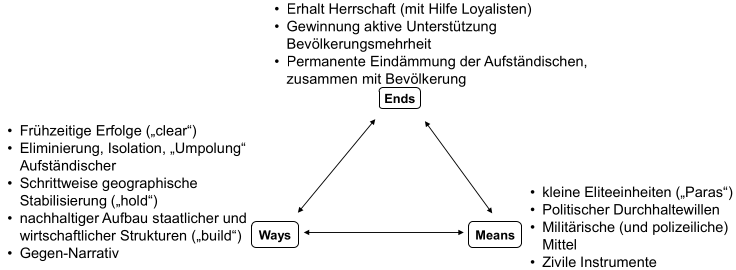
\includegraphics{images/trinquier.png} \emph{Schematische Einordnung des
	französischen Ansatzes}

\subsubsection{Technologie und COIN in Vietnam
	1965-1975}\label{technologie-und-coin-in-vietnam-1965-1975}

\begin{itemize}
	\tightlist
	\item
	      Luftaufklärung? (links,o)
	\item
	      Agent Orange (links,u)
	\item
	      Schnüffelgerät (mitte,o)
	\item
	      Abholzung (mitte,u)
	\item
	      Versorgung durch \textbf{Ho-Chi-Minh-Pfad} (rechts)
\end{itemize}

\begin{figure}
	\centering
	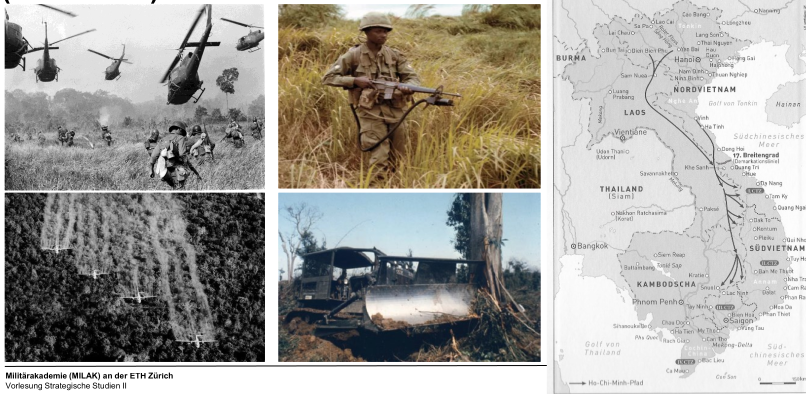
\includegraphics{images/vietnam.png}
	\caption{vietnam}
\end{figure}

\subsubsection{Aufstandsbekämpfung im Kalten
	Krieg}\label{aufstandsbekuxe4mpfung-im-kalten-krieg}

\begin{itemize}
	\tightlist
	\item
	      Referenzwerke für moderne COIN-Theorien
	\item
	      Zunehmend konstruktiver Einbezug lokale Bevölkerung
	\item
	      Erkenntnis, dass konventionelle Kriegführung gegen irregulären Gegner
	      nicht erfolgversprechend ist
	\item
	      Erkenntnis, dass Erfolg der Guerilla bei externer, konventioneller
	      Unterstützung steigt
	\item
	      Häufig: Unterschätzung des Gegners
\end{itemize}

\subsubsection{COIN: US-Zwischenbilanz
	2006}\label{coin-us-zwischenbilanz-2006}

\begin{itemize}
	\tightlist
	\item
	      FM 3-24: ``The People-centric Approach''
	\item
	      Einsätze in 4 Phasen: 1. Shape 2. Clear 3. Hold 4. Build
\end{itemize}

\subsubsection{Fazit und Kritik: Das Ende von
	Coin?}\label{fazit-und-kritik-das-ende-von-coin}

\begin{itemize}
	\tightlist
	\item
	      COIN-Erfahrungen häufig selektiv und idealisiert
	\item
	      COIN-Erfolg abhängig von Verhältnissen im Zielland: Regierung muss
	      Legitimität bei Zivilbevölkerung primär selbst schaffen
	\item
	      Streitkräfte wenig geeignet für ``build''-Komponenten von COIN
	\item
	      Vorwürfe an moderne COIN-Konzeptionen:

	      \begin{itemize}
		      \tightlist
		      \item
		            COIN unterstütze westliche politische Agenden der Expansion
		            (verdeckter Imperialismus)
		      \item
		            COIN schwäche Fähigkeit von Streitkräften zur konventionellen
		            Kriegführung (Kernkompetenz)
		      \item
		            COIN zu kostspielig und von fragwürdiger Nachhaltigkeit
	      \end{itemize}
	\item
	      Erfolgsbilanz derzeit nicht besonders gut, politischer Wille für COIN
	      tief
	\item
	      Trotzdem bleibt irreguläre Kriegführung sowie Aufstandsbekämpfung auch
	      im Schatten des derzeitigen Grossmachtwettbewerbs relevant
\end{itemize}

\subsection{Die strategische Bedeutung von
	Kriegsgefangenen}\label{die-strategische-bedeutung-von-kriegsgefangenen}

mit Dr.~Tamara Cubito

\subsubsection{Leitfragen}\label{leitfragen-6}

\begin{itemize}
	\tightlist
	\item
	      Welche strategische Bedeutung kommt Kriegsgefangenen in regulären und
	      irregulären Konstellationen zu?
	\item
	      Wie müssen Kriegsgefangene nach dem Völkerrecht behandelt werden?
	\item
	      Welche Rolle kommt dem IKRK zu?
\end{itemize}

\begin{quote}
	What is a prisoner of war? He is a man who tries to kill you and fails,
	and then asks you, not to kill him.\\
	- \emph{Winston Churchill (zugeschrieben)}
\end{quote}

\subsubsection{Lektüre}\label{lektuxfcre-6}

\begin{itemize}
	\tightlist
	\item
	      Sibylle Scheipers, Introduction: Prisoners in War, in: Sibylle
	      Scheipers (Hg.), Prisoners in War, New York 2010, S. 1-3, 7-16.
	\item
	      Sibylle Scheipers, Conclusion: Prisoners and Detainees in Current and
	      Future Military Operations, in: Sibylle Scheipers (Hg.), Prisoners in
	      War, New York 2010, S. 313-318.
\end{itemize}

\subsubsection{Mannigfaltige
	Bedeutungen}\label{mannigfaltige-bedeutungen}

\begin{itemize}
	\item
	      Je nach Konfliktlogik und -parteien kommen Kriegsgefangenen ganz
	      unterschiedliche Bedeutungen zu
	\item
	      Die neuere Forschung sieht Kriegsgefangene nicht länger ``nur'' als
	      Opfer, sondern zunehmend als Akteure, Ressourcen und Spiegel der
	      Ideologie(n)
\end{itemize}

\subsubsection{Bis zum 19. Jahrhundert}\label{bis-zum-19.-jahrhundert}

\begin{itemize}
	\tightlist
	\item
	      ``Range'' an Optionen: Exekution, Versklavung, Gefangenschaft,
	      Freilassung, Freikauf, Austausch, Parole, Eingliederung in die eigenen
	      Streitkräfte
	\item
	      Gebräuche und Abmachungen, keine verbindlichen Gesetze und Regeln
	\item
	      Kaum Kriegsgefangenenlager
	\item
	      Wichtig: Unterschiede Offiziere-Soldaten
	\item
	      ab 19. Jahrhundert: Beginn ``moderner'' Kriegsgefangenschaft
\end{itemize}

\subsubsection{Erste internationale
	Abkommen}\label{erste-internationale-abkommen}

\paragraph{General Orders No.~100
	(1863)}\label{general-orders-no.-100-1863}

\begin{itemize}
	\tightlist
	\item
	      Regelungen im US Civil War von Francis Lieber (1800-1872)
\end{itemize}

\begin{quote}
	A prisoner of war is subject to no punishment for being a public enemy,
	nor is any revenge wreaked upon him by the intentional infliction of any
	suffering, or disgrace, by cruel imprisonment, want of food, by
	mutilation, death, or any other barbarity.\\
	\emph{General Orders No.~100, Artikel 56}
\end{quote}

\begin{itemize}
	\tightlist
	\item
	      157 Artikel untersagen als Vorläufer der Genfer Konvention Folter und
	      unmenschliche Behandlung
	\item
	      Kriegsgefangenschaft als Schutz-, nicht Strafmassnahme
	\item
	      Definition der Freilassungs- oder Austauschregelungen
\end{itemize}

\paragraph{Wichtiger Wendepunkt:
	1870/71}\label{wichtiger-wendepunkt-187071}

\begin{itemize}
	\tightlist
	\item
	      Bis dahin unvorstellbare Anzahl POWs (Bis Ende 1870: über 340'000 frz.
	      POWs)
	\item
	      Preussischer Generalstabschef von Moltke bestand auf Gefangenschaft:
	      Entzug Kampfkraft
	\item
	      Regulativ über die Behandlung, Verpflegung der Kriegsgefangenen nach
	      erfolgtem Eintreffen in den Gefangenendepots
	\item
	      Sold, Kost und Logis
	\item
	      Sonderbehandlung von Offizieren (z.B.Ehrenwort, Unterkunft, Bezahlung)
	\item
	      Erstmalige Lagerbesuche und Involvierung internationaler
	      Organisationen, z.B. IKRK
	\item
	      Unklarheiten bei Kriegsgefangenenstatus von Franc-Tireurs
	\item
	      Konklusion: Es braucht ein internationales Abkommen!
\end{itemize}

\paragraph{Haager Landkriegsordnung}\label{haager-landkriegsordnung}

Haager Friedenskonferenzen 1899 \& 1907 in Den Haag

\begin{itemize}
	\tightlist
	\item
	      Aufklärerische und pazifistische Akteure wollen den Krieg einschränken
	      und/oder ``humanisieren''
	\item
	      Vage Definitionen zu Kombattanten und Kriegsgefangenen
	\item
	      Grundsatz: Unbedingte Verschonung sich ergebender Gegner und deren
	      angemessene Behandlung
	\item
	      Artikel 4: ``Die Kriegsgefangenen unterstehen der Gewalt der
	      feindlichen Regierung, aber nicht der Gewalt der Personen oder der
	      Korps, die sie gefangengenommen haben. Sie sollen mit Menschlichkeit
	      behandelt werden. Alles, was ihnen persönlich gehört, verbleibt ihr
	      Eigentum mit Ausnahme von Waffen, Pferden und Schriftstücken
	      militärischen Inhalts.''
\end{itemize}

\subsubsection{Erster Weltkrieg}\label{erster-weltkrieg}

\paragraph{Ein paar Zahlen}\label{ein-paar-zahlen}

\begin{itemize}
	\tightlist
	\item
	      Insgesamt: 6,6-8,4 Mio. Kriegsgefangene an allen Fronten (ca. 1 von 8
	      Soldaten)
	\item
	      Grosse Unterschiede nach Kriegsschauplätzen/Nationen (z.B.
	      Österreich-Ungarn: 1 von 3)
\end{itemize}

\paragraph{Probleme in der Praxis}\label{probleme-in-der-praxis}

\begin{itemize}
	\item
	      Ab wann ein POW?

	      \begin{quote}
		      We were held up by machine-gun fire from a ridge\ldots{} I don't know
		      how I escaped because I was lying right out in the front. After losing
		      half of my company there, we rushed them and they had the nerve to
		      throw up their hands and cry, ``Kamerad'' All the ``Kamerad'' they got
		      was a foot of cold steel thro them from my remaining men while I blew
		      their brains out with my revolver without any hesitation. You may
		      think this rather rough but if you had seen my boys go down you would
		      have done the same and my only regret is that too many prisoners are
		      taken.\\
		      \emph{Lieutenant R.C. Germain, 20th Canadian Infantry Battalion}
	      \end{quote}
\end{itemize}

\paragraph{Propaganda}\label{propaganda}

\begin{itemize}
	\tightlist
	\item
	      Einsatz zum motivieren der eigenen und demotivieren der gegnerischen
	      Armee und Bevölkerung.
\end{itemize}

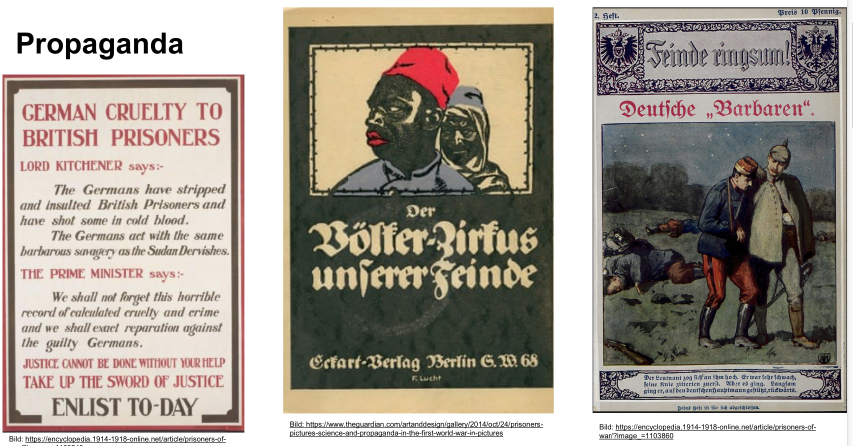
\includegraphics{images/pow-propaganda.png} \emph{CAPTION}

\paragraph{Politische Instrumente}\label{politische-instrumente}

\begin{itemize}
	\tightlist
	\item
	      Reziprozität: Bessere Bedingungen für eigene Kriegsgefangene
	\item
	      Möglichst viele Kriegsgefangene ein Vorteil
	\item
	      Aber: Funktioniert nur, wenn ein Staat am Wohlergehen seiner
	      Kriegsgefangenen interessiert ist (Bsp. Italien)
	\item
	      Druckmittel für Unterzeichnung des Friedensabkommens nach Kriegsende
\end{itemize}

\paragraph{Zeichen des militärischen
	Erfolgs}\label{zeichen-des-milituxe4rischen-erfolgs}

\begin{itemize}
	\tightlist
	\item
	      Wie wird Erfolg gemessen?
	\item
	      Grabenkrieg: Kriegsgefangene als Beweis für Erfolg an einer Front ohne
	      grosse Gebietsgewinne
	\item
	      ?Motivation?
\end{itemize}

\paragraph{Arbeitskräfte}\label{arbeitskruxe4fte}

\begin{itemize}
	\tightlist
	\item
	      Arbeit explizit erlaubt
	\item
	      DR: 2,5 Mio. Kriegsgefangene bis Kriegsende; 90\% davon als
	      Arbeitskräfte eingesetzt (hauptsächlich Landwirtschaft und Industrie
	      inkl. Munitionsproduktion)
	\item
	      1918: 18\% aller Kohlearbeiter im Ruhrgebiet Kriegsgefangene
	\item
	      Trotz Verbot: Hunderttausende Kriegsgefangene an Front eingesetzt,
	      z.B. Grabenbau
	\item
	      Nach Kriegsende: Für Wiederaufbau eingesetzt
\end{itemize}

\subsubsection{Genfer Konventionen}\label{genfer-konventionen}

\paragraph{Erstes Abkommen 1929}\label{erstes-abkommen-1929}

\begin{itemize}
	\tightlist
	\item
	      Abkommen über die Behandlung von Kriegsgefangenen
	\item
	      Bis dato umfassendste Kodifikation des Kriegsgefangenenrechts
	\item
	      Völkerrechtliche Akzeptanz des IKRK
\end{itemize}

\paragraph{Anpassung 1949}\label{anpassung-1949}

\begin{itemize}
	\tightlist
	\item
	      Völkerrechtliche Zäsur durch Genfer Konvention 1949
	\item
	      Ersetzt das 1929er Abkommen
\end{itemize}

\paragraph{Dritte Konvention 19??}\label{dritte-konvention-19}

\begin{itemize}
	\tightlist
	\item
	      Konvention bezüglich der Behandlung von Kriegsgefangenen
	\item
	      Verbietet insbesondere Tötung, Gefährdung, Gewaltanwendung, Folter,
	      Verstümmelung, Experimente, Bedrohung, Beleidigung, Erniedrigung,
	      öffentliches Zurschaustellen, Repressalien sowie Vergeltungsmassnahmen
\end{itemize}

\subsubsection{Zweiter Weltkrieg}\label{zweiter-weltkrieg}

\paragraph{Kriegsgefangene 1937-1945}\label{kriegsgefangene-1937-1945}

\begin{itemize}
	\tightlist
	\item
	      Insgesamt mind. 35 Mio. Kriegsgefangene
	\item
	      Je nach Kriegsphase ungleiche Gefangenenzahlen
	\item
	      Bsp. Barbarossa: 30'000 deutsche POWs vs.~3,35 Mio. sowjetische POWs
	      innert 6 Monaten)
	\item
	      Extreme Unterschiede je nach Kriegsschauplatz; entsprechend auch
	      unterschiedliche strategische Bedeutung
	\item
	      Relevanz ``rassistischer'' Elemente für die Kriegsgefangenschaft, z.B.
	      chinesische POWs
	\item
	      Hohe Todesraten: Von 9 Mio. POWs an Ostfront verstarben bspw. 4 Mio.
	      in Gefangenschaft
	\item
	      Mehr Durchhaltewillen aufgrund von Angst vor Kriegsgefangenschaft?
\end{itemize}

\paragraph{Probleme in der Praxis}\label{probleme-in-der-praxis-1}

\begin{itemize}
	\tightlist
	\item
	      Wer ist ein Kriegsgefangener?
	\item
	      Kolonialtruppen oder Freie Franzosen von Deutschen nicht als reguläre
	      Soldaten anerkannt
	\item
	      Handelsmarine: POWs für die Deutschen, Zivilisten für die Briten
	\item
	      Was passiert mit POWs nach ``Seitenwechsel''? (Bsp.: Italien 1943)
	\item
	      Drittes Reich: Einzelne sowjetische Soldaten oder kleine Gruppen =
	      Partisanen
\end{itemize}

\paragraph{Arbeitskräfte}\label{arbeitskruxe4fte-1}

\begin{itemize}
	\tightlist
	\item
	      Deutsche und Italiener in Landwirtschaft, Bauindustrie (zivil) und
	      Forstwirtschaft in GB
	\item
	      Italienische POWs bauten Strassen und halfen in der südafrikanischen
	      Landwirtschaft
	\item
	      Australier, Briten und Inder für den Bau einer Eisenbahnlinie in
	      Burma/Thailand
	\item
	      Oft je nach Verlauf des Krieges; z.B. Italienische POWs der USA in
	      Nordafrika zuerst vor Ort eingesetzt (z.B. Transport, Strassenbau) und
	      nach Ende der Kampagne in den USA
\end{itemize}

\subparagraph{Beispiel Drittes Reich}\label{beispiel-drittes-reich}

\begin{itemize}
	\tightlist
	\item
	      Ab 1939: Polnische POWs (Sommer 1940: ca. 400'000), dann
	      ``Statuswechsel''
	\item
	      Frankreich: POWs ausgetauscht, ``Statuswechsel'' oder gem. Genfer
	      Konventionen als POWs
	\item
	      Ab 1941: Sowjetische POWs
	\item
	      Ab 1943: 600'000 italienische ``Verräter''
\end{itemize}

\paragraph{Rekrutierungspool}\label{rekrutierungspool}

\begin{itemize}
	\tightlist
	\item
	      Bsp. Polnische POWs der Sowjets (2 Korpus Polski)
	\item
	      Bsp. Drittes Reich:

	      \begin{itemize}
		      \tightlist
		      \item
		            Ab Juli 1941: Selektionierte sowjetische Hiwis in Wehrmacht als
		            Ersatz
		      \item
		            ``Osttruppen'' teils in Wehrmacht integriert, teils separate
		            Einheiten
		      \item
		            Verschiedenste Rollen, insgesamt 1-1,3 Mio.
	      \end{itemize}
	\item
	      Bsp. Japan: INA
\end{itemize}

\paragraph{Objekte der Indoktrination}\label{objekte-der-indoktrination}

Indoktrination und Politische Instrumentalisierung

\begin{itemize}
	\tightlist
	\item
	      Gescheiterte sowjetische Indoktrination polnischer Offiziere: Massaker
	      von Katyn
	\item
	      Entnazifizierung in den USA und Grossbritannien

	      \begin{itemize}
		      \tightlist
		      \item
		            Mit Facts, Filmen, Zeitungen, Vorträgen etc. überzeugen
		      \item
		            ``Nazi''-Literatur aus Lagern entfernt und ersetzt mit
		            ``verbotenen'' Büchern
		      \item
		            Trennung von Gefangenen, Unterstützung von ``anti-Nazi'' POWs
	      \end{itemize}
	\item
	      Bedeutung von POWs in der ``Flamenpolitik'' des Dritten Reichs
	\item
	      Sowjetunion: Indoktrination zweitrangig
\end{itemize}

\paragraph{Propaganda}\label{propaganda-1}

\begin{itemize}
	\tightlist
	\item
	      ``Positive'' Propaganda weniger bedeutend als im Ersten Weltkrieg
	\item
	      Beispiel Japan: Weisse POWs, um japanische Überlegenheit zu
	      ``beweisen''
\end{itemize}

\paragraph{Nach dem Krieg}\label{nach-dem-krieg}

• Kriegsgefangene in grösserem Ausmass als 1914-18 für Wiederaufbau und
Arbeiten nach Kriegsende eingesetzt • Nicht mehr POWs, sondern
``surrendered military personnel'' • Wurden von Alliierten in Europa
``verteilt'' • Japanische ex-Soldaten in aufflammenden Kriegen in
Kolonien eingesetzt

\paragraph{Fazit Zweiter Weltkrieg}\label{fazit-zweiter-weltkrieg}

Jegliche Abkommen betreffend Kriegsgefangener nutzlos?

\subsubsection{Wer ist
	Kriegsgefangener?}\label{wer-ist-kriegsgefangener}

Gemäss \textbf{Genfer Abkommen} über die Behandlung der
Kriegsgefangenen,

\textbf{Artikel 4}: Kriegsgefangene im Sinne des vorliegenden Abkommens
sind die in die Gewalt des Feindes gefallenen Personen, die einer der
nachstehenden Kategorien angehören:

\begin{itemize}
	\tightlist
	\item
	      Angehörige von bewaffneten Kräften einer am Konflikt beteiligten
	      Partei, ebenso Angehörige von Milizen und Freiwilligenkorps, die zu
	      diesen bewaffneten Kräften gehören
	\item
	      Angehörige anderer Milizen und Freiwilligenkorps, einschliesslich
	      solcher von organisierten Widerstandsbewegungen, die zu einer am
	      Konflikt beteiligten Partei gehören und ausserhalb oder innerhalb
	      ihres eigenen Gebietes, auch wenn dasselbe besetzt ist, tätig sind,
	      sofern diese Milizen oder Freiwilligenkorps, einschliesslich der
	      organisierten Widerstandsbewegungen:

	      \begin{itemize}
		      \tightlist
		      \item
		            an ihrer Spitze eine für ihre Untergebenen verantwortliche Person
		            haben
		      \item
		            ein bleibendes und von weitem erkennbares Zeichen tragen
		      \item
		            die Waffen offen tragen
		      \item
		            bei ihren Operationen die Gesetze und Gebräuche des Krieges
		            einhalten
	      \end{itemize}
	\item
	      Angehörige regulärer bewaffneter Kräfte, die sich zu einer von der
	      Gewahrsamsmacht nicht anerkannten Regierung oder Behörde bekennen
	\item
	      Personen, die den bewaffneten Kräften folgen {[}\ldots{]}
	\item
	      Besatzungsmitglieder der Handelsmarine {[}\ldots{]}
	\item
	      die Bevölkerung eines unbesetzten Gebietes, die beim Herannahen des
	      Feindes aus eigenem Antrieb die Waffen gegen die Invasionstruppen
	      ergreift, ohne zur Bildung regulärer Streitkräfte Zeit gehabt zu
	      haben, sofern sie die Waffen offen trägt und die Gesetze und Gebräuche
	      des Krieges einhält.'' {[}\ldots{]}
\end{itemize}

\paragraph{Info}\label{info}

Auch irreguläre Kombattanten müssen als POWs behandelt werden, bis ihnen
ein Kriegsgericht den Kriegsgefangenenstatus abspricht!

\subsubsection{POWs als Quelle für
	Informationen}\label{pows-als-quelle-fuxfcr-informationen}

\begin{itemize}
	\tightlist
	\item
	      POWs müssen lediglich

	      \begin{itemize}
		      \tightlist
		      \item
		            Name,
		      \item
		            Dienstgrad,
		      \item
		            Geburtsdatum
		      \item
		            und Erkennungsnummer preisgeben
	      \end{itemize}
	\item
	      Alles Weitere dürfen sie verweigern
	\item
	      Verhöre sind erlaubt, dürfen aber nicht zu physischen oder
	      psychologischen Schäden führen
	\item
	      Befragung durch militärisch geschultes Personal:

	      \begin{itemize}
		      \tightlist
		      \item
		            Vertauensaufbau, Aushorchung, psychologische Techniken
	      \end{itemize}
	\item
	      Verbot von Bestrafungen
\end{itemize}

\subsubsection{POWs in der Schweizer
	Armee}\label{pows-in-der-schweizer-armee}

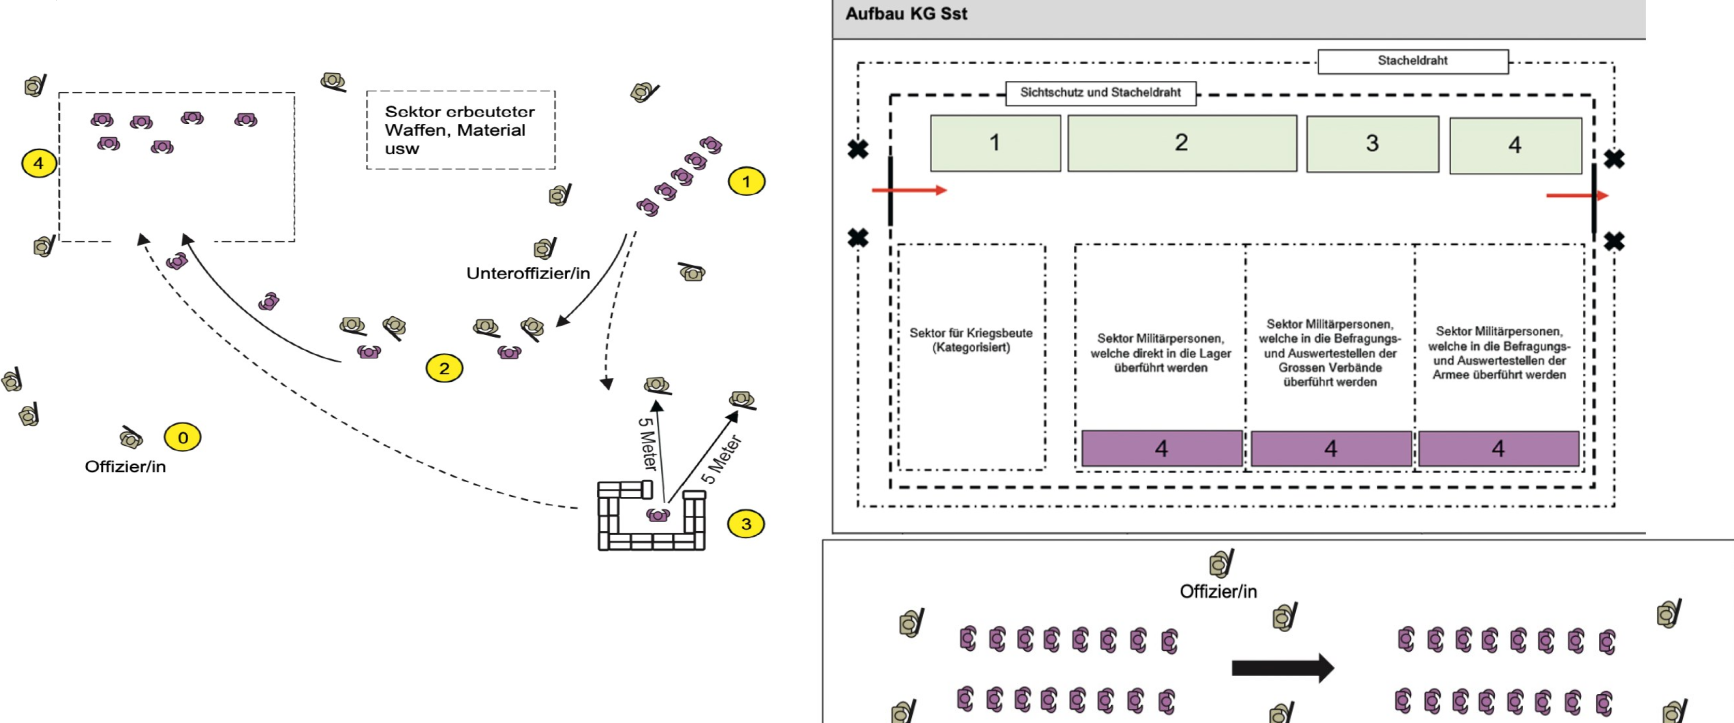
\includegraphics{images/pow-sa.png} \emph{Kdo Op, FGG1, Reglement
	Kriegsgefangenen- und Interniertenwesen, Bern, 2024, S.21,26}

\subsubsection{Fazit}\label{fazit-3}

\begin{itemize}
	\tightlist
	\item
	      Reglementierung und Systematisierung des POW-Status, der Rechte und
	      Pflichten mit sich bringt
	\item
	      Problematik der Abgrenzung POWs vs zivile Gefangene
	\item
	      Mannigfaltige strategische Bedeutungen von Kriegsgefangenen: Vom
	      Informationsträger über die politische und diplomatische Symbolik bis
	      zur Verhandlungsmasse
	\item
	      Über die Behandlung von Gefangenen lernen wir viel über die
	      strategische Kultur einer Streitkraft / eines Landes
\end{itemize}

\subsection{Kriegslogistik}\label{kriegslogistik}

mit Dr.~Ronald Ti

\subsubsection{Leitfragen}\label{leitfragen-7}

\begin{itemize}
	\tightlist
	\item
	      Wie hat sich die moderne Kriegslogistik entwickelt?
	\item
	      Wie interagieren militärstrategische Prinzipien mit der
	      Kriegslogistik?
	\item
	      Welche Rolle spielt die Kriegslogistik im Ukrainekrieg?
\end{itemize}

\subsubsection{Lektüre}\label{lektuxfcre-7}

\begin{itemize}
	\tightlist
	\item
	      Ronald Ti/Christopher Kinsey, Lessons from the Russo-Ukrainian
	      Conflict: The Primacy of Logistics over Strategy, in: Defence Studies,
	      Vol. 23 (3), 2023, S. 381-398.
\end{itemize}

\subsubsection{Ziel der Gastvorlesung}\label{ziel-der-gastvorlesung}

\begin{itemize}
	\item
	      Einführung in die logistische Planung von Expeditionen in einem Joint
	      Force Hauptquartier
	\item
	      Besprechung von Kontingenzoperationen / Non-Article V Crisis Response
	      Operations (NA5CRO's) aber \textbf{nicht} stationäre Operationen wie
	      UNIFIL/ UNDOF.

	      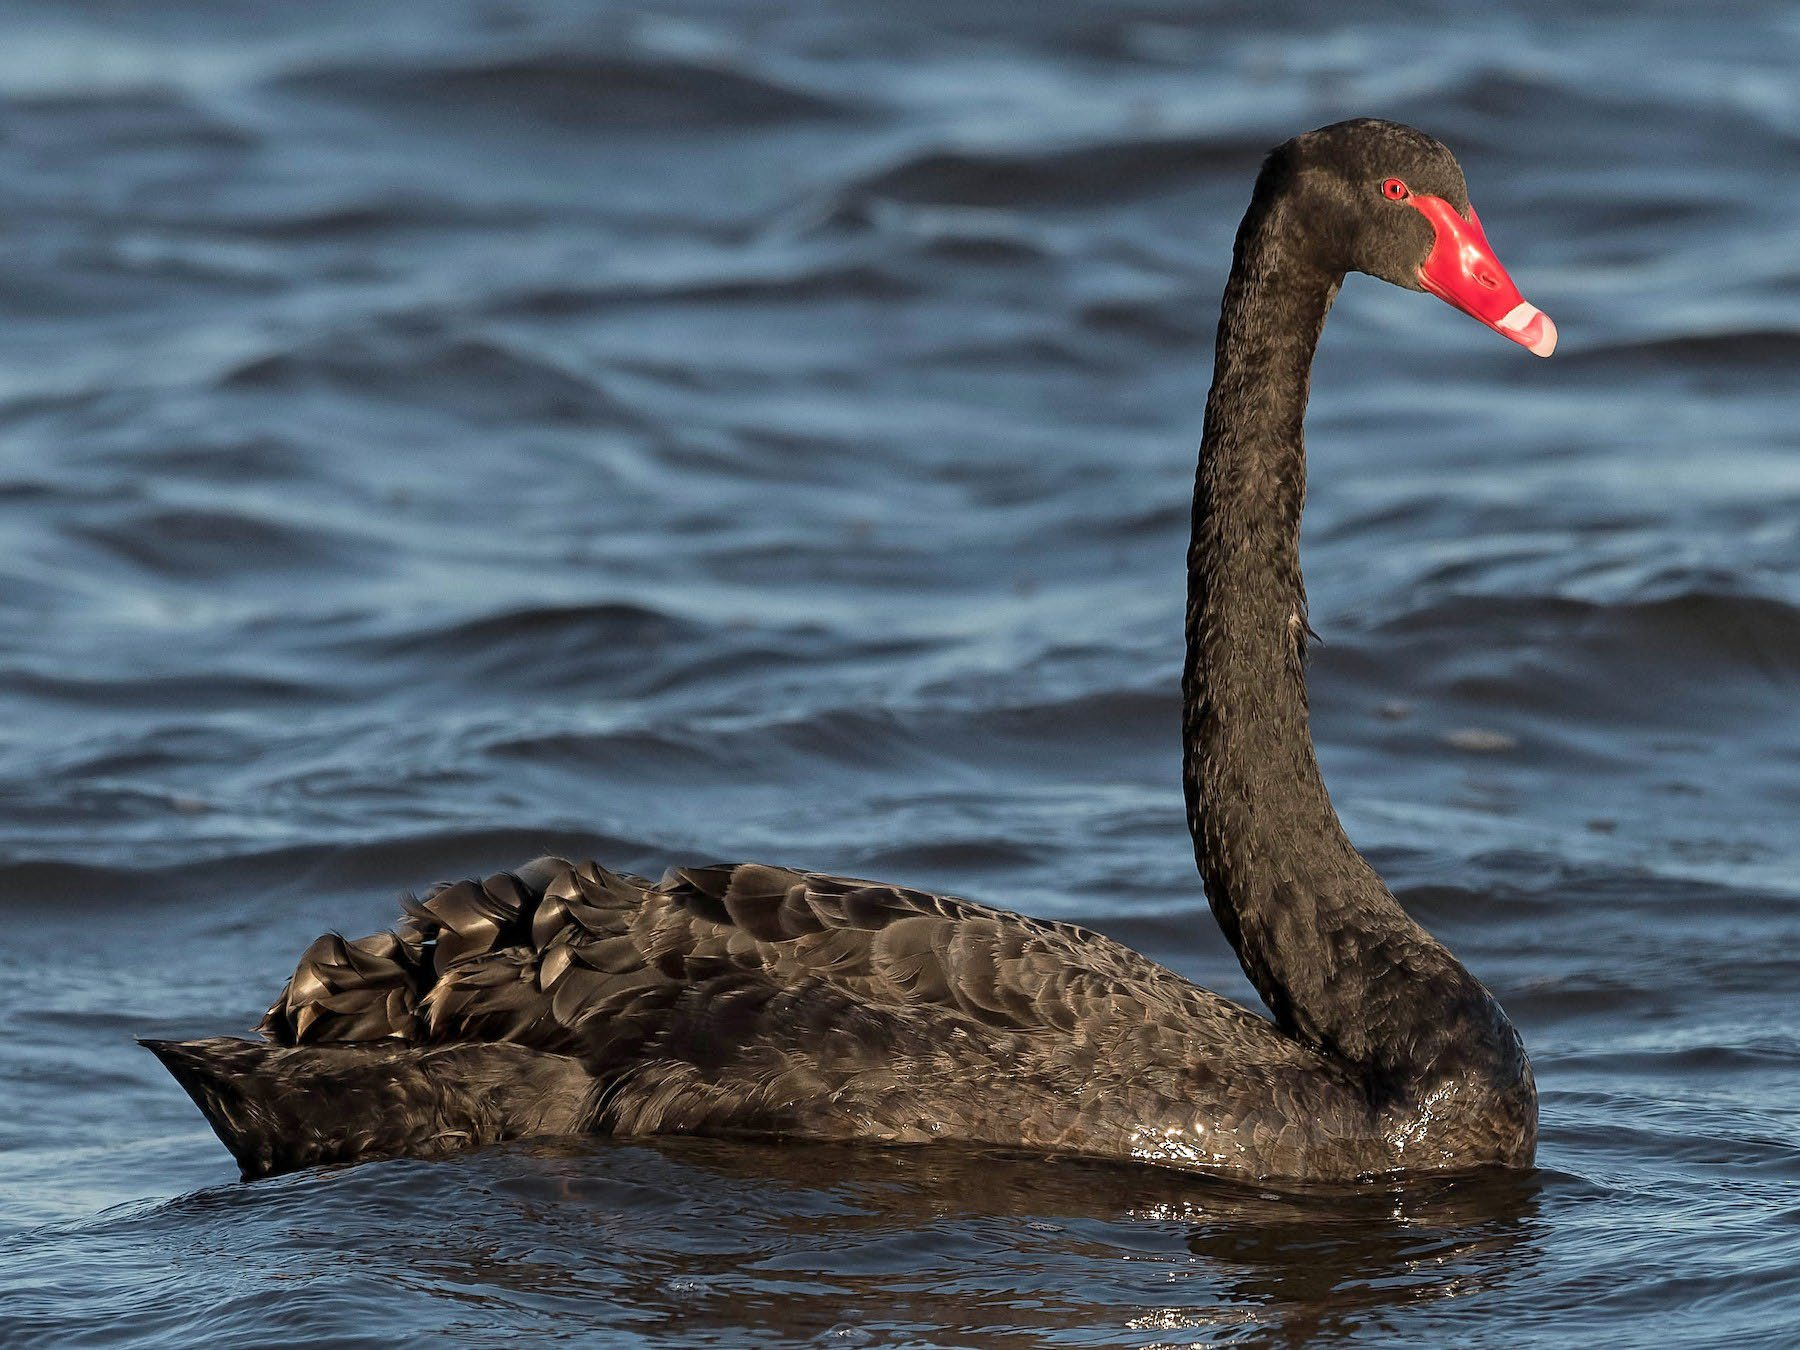
\includegraphics{images/swan.png} \emph{Be the swan\ldots{}}
	      \textbf{?}
\end{itemize}

\subsubsection{5 D der Logistik}\label{d-der-logistik}

\paragraph{Destination - Zielort}\label{destination---zielort}

\begin{itemize}
	\tightlist
	\item
	      Standplatz, Infrastruktur

	      \begin{itemize}
		      \tightlist
		      \item
		            Humanitarian Assistance Disaster Relief (HADR) Operationen häufig in
		            kurz zuvor umkämpften Regionen
		      \item
		            Gute Infrastruktur ist rar
		      \item
		            Benötigt Militäringenieure zum Aufbau
		      \item
		            Benötigt Militäringenieure zum Räumen von explosiven Überresten
	      \end{itemize}
	\item
	      Air Point of Disembarktion (APOD)

	      \begin{itemize}
		      \tightlist
		      \item
		            Landebahn oder Flugplatz
		      \item
		            Logistischer Fluss nicht nur durch verfügbare Flugzeuge vorgegeben
		      \item
		            Benötigt Säuberung von Blindgängern und Minen
		      \item
		            Benötigt Unterhalt und Reperaturen
	      \end{itemize}
	\item
	      Sea Point of Disembarkation (SPOD)

	      \begin{itemize}
		      \tightlist
		      \item
		            Muss von Minen gesäubert sein
		      \item
		            Kann blockiert sein und muss ausgebaggert werden
		      \item
		            Hafeninfrastruktur zerstört
	      \end{itemize}
	\item
	      Beach

	      \begin{itemize}
		      \tightlist
		      \item
		            Gezeiten, Wellen, eventuell knappes Zeitfenster
		      \item
		            Riffe können Weg blockieren, Sprengen oder Luftkissenlandungsboot
	      \end{itemize}
\end{itemize}

\paragraph{Distance}\label{distance}

\begin{itemize}
	\tightlist
	\item
	      Kommunikationslinien (LOC) können sehr lang werden
	\item
	      Risiko Management, was ist akzeptierbar?
\end{itemize}

\begin{longtable}[]{@{}
	>{\raggedright\arraybackslash}p{(\columnwidth - 2\tabcolsep) * \real{0.2041}}
	>{\raggedright\arraybackslash}p{(\columnwidth - 2\tabcolsep) * \real{0.7959}}@{}}
	\toprule\noalign{}
	\begin{minipage}[b]{\linewidth}\raggedright
		Zeit nach Verletzung
	\end{minipage} & \begin{minipage}[b]{\linewidth}\raggedright
		                 Behandlung
	                 \end{minipage}                                           \\
	\midrule\noalign{}
	\endhead
	\bottomrule\noalign{}
	\endlastfoot
	10 Minuten                                  & Kontrolle größerer Blutungen und Atemwege               \\
	1 Stunde                                    & Vorgezogene Wiederbelebungsmaßnahmen, unterwegs oder in
	Gesundheitseinrichtung                                                                                \\
	2 Stunden                                   & Operationen in einer dafür ausgestatteten Einrichtung   \\
\end{longtable}

\paragraph{Demand}\label{demand}

\begin{itemize}
	\tightlist
	\item
	      Push and Pull Logistics

	      \begin{itemize}
		      \tightlist
		      \item
		            Grundsätzlich Push-Logistik in Anfangsphase, besonders Treibstoff
		            und Munition (Class V, Class III)
		      \item
		            Pull-Logistik typischerweise bei Personalsupport, Medizinische
		            Versorgung, (Class VIII)
	      \end{itemize}
	\item
	      Wasser

	      \begin{itemize}
		      \tightlist
		      \item
		            Grundwasser reinigen, Reverse Osmosis Purification Units (ROPU's)
		      \item
		            Gesundheitsschutz, Benötigt medizinische Infrastruktur
	      \end{itemize}
\end{itemize}

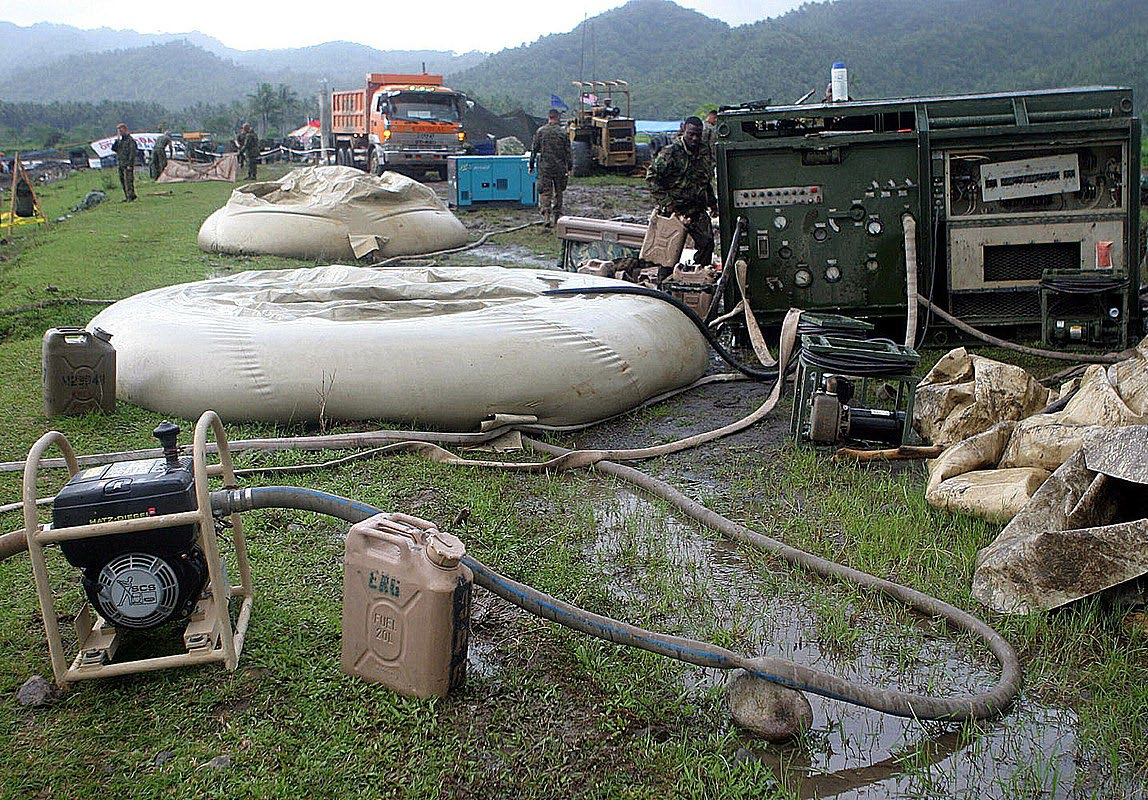
\includegraphics{images/water.png} \emph{CAPTION}

\paragraph{Duration}\label{duration}

\begin{itemize}
	\tightlist
	\item
	      Aufrechterhaltung von Standort

	      \begin{itemize}
		      \tightlist
		      \item
		            Personal
		      \item
		            Zulieferer
		      \item
		            eventuell internationale Partner
	      \end{itemize}
\end{itemize}

\paragraph{Dependency}\label{dependency}

\begin{itemize}
	\tightlist
	\item
	      Verträge mit Zulieferern und Dienstleistern weit verbreitet,
	      Contractor Support on Operations(CSO)
	\item
	      Diese sind technisch gesehen keine Kombattanten, aber im Kriegsgebiet
\end{itemize}

\subsubsection{Doktrin}\label{doktrin}

\begin{itemize}
	\tightlist
	\item
	      Im Zweifelsfall in der Doktrin nachschauen
	\item
	      Doktrin Lesen und Doktrin Anwenden
	\item
	      80/20 Kurzregel der Logistik

	      \begin{itemize}
		      \tightlist
		      \item
		            80\% ist Risikominimierung, die verbleibenden 20\% sind das Risiko.
	      \end{itemize}
	\item
	      GNLC Logistic Handbook, 2010
	\item
	      Beispiele

	      \begin{itemize}
		      \tightlist
		      \item
		            Australian doctrine is very readable
		      \item
		            US doctrine is unreadable
		      \item
		            NATO doctrine is watered down
		      \item
		            UK doctrine is ok
	      \end{itemize}
\end{itemize}

\subsubsection{5 Lektionen aus der
	Ukraine}\label{lektionen-aus-der-ukraine}

\paragraph{Tactical and operational effects of
	UAS}\label{tactical-and-operational-effects-of-uas}

\subparagraph{FPV Drohnen}\label{fpv-drohnen}

\begin{itemize}
	\tightlist
	\item
	      Geschwindigkeit 160km/h
	\item
	      Lauern um Panzer und Bunker
	\item
	      Alle Komponenten einfach Verfügbar
	\item
	      Ukrainische Angriffszone, 10km Radius, 1500m Höhe
\end{itemize}

\subparagraph{Preisvergleich}\label{preisvergleich}

\begin{longtable}[]{@{}ll@{}}
	\toprule\noalign{}
	Typ               & Preis (CHF) \\
	\midrule\noalign{}
	\endhead
	\bottomrule\noalign{}
	\endlastfoot
	Artilleriegranate & 717-894     \\
	Excalibur         & 89'000      \\
	Javlin            & 178'000     \\
	Drohne            & 358         \\
\end{longtable}

\subparagraph{Eigenschaften FPV
	Drohnen}\label{eigenschaften-fpv-drohnen}

\begin{itemize}
	\tightlist
	\item
	      Trefferquote 10-80\% (nicht alle explodieren)
	\item
	      Statische Radiofrequenz kann gestört werden
	\item
	      \textbf{Improved terminal guidance} Software-basierte Funkempfänger
	      ermöglichen einfacheren Frequenzwechsel
	\item
	      Benötigt Piloten mit Training und Erfahrung und
	      Unterstützungseinheiten
\end{itemize}

\subparagraph{Glasfaser FPV Drohnen}\label{glasfaser-fpv-drohnen}

\begin{itemize}
	\tightlist
	\item
	      Steuerungssignal über Kabel das von Spule in Drohne abgewickelt wird
	\item
	      Reichweite 20km, in einem Wald bis zu 15km
	\item
	      Kann nicht gestört werden durch elektronische Gegenmassnahmen
	\item
	      Hochauflösende Datenübertragung über optischen Leiter
\end{itemize}

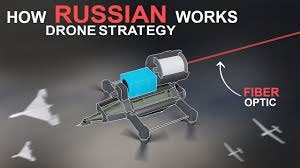
\includegraphics{images/optic.png}\\
\emph{Funktionsprinzip der mit Glasfaser optisch gesteuerten Drohnen}

\subparagraph{Autonome Drohne}\label{autonome-drohne}

\begin{itemize}
	\tightlist
	\item
	      Einwegdrohne
	\item
	      Video Ukrainer
	      \href{https://www.youtube.com/watch?v=tLUmv9TO9xU}{hier}
	\item
	      3kg Sprengstoff, bis zu 12km
	\item
	      Ask: difference between kill chain and kill web?
\end{itemize}

\subparagraph{Operational level
	systems}\label{operational-level-systems}

Bayraktar TB2

\begin{itemize}
	\tightlist
	\item
	      Reichweite 150km
	\item
	      Flughöhe 8km
	\item
	      Flughöhe 4.5km
	\item
	      Einsatzdauer 27h
\end{itemize}

\begin{figure}
	\centering
	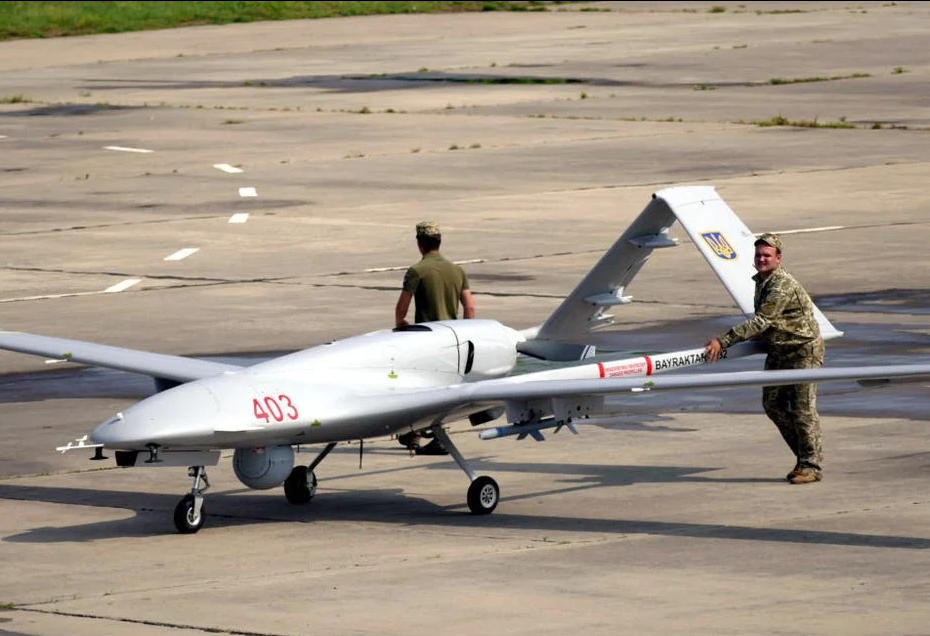
\includegraphics{images/bayraktar.png}
	\caption{bayraktar}
\end{figure}

Harop

\begin{itemize}
	\tightlist
	\item
	      Reichweite 1000km
	\item
	      Einsatzdauer 9h
	\item
	      Preis \textless{} \$500k
	\item
	      Erwartete Systemzeit 13 Jahre
	\item
	      Komplett autonom
	\item
	      Gewicht 40kg
\end{itemize}

\begin{figure}
	\centering
	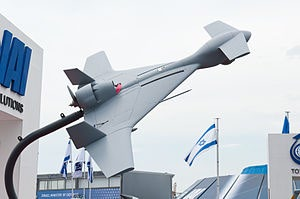
\includegraphics{images/harop.png}
	\caption{harop}
\end{figure}

\subparagraph{Medium Altitude Long Endurance (MALE)
	systems}\label{medium-altitude-long-endurance-male-systems}

\begin{itemize}
	\tightlist
	\item
	      DX3, VTOL UAS: \$200,000, 3 m wingspan, 1,500 km range
	\item
	      QXX 222, VTOL, 0.85 Mach, can carry 2 x 250 kg bombs up to 2500 km
\end{itemize}

\paragraph{Transparent tactical
	battlespace}\label{transparent-tactical-battlespace}

\begin{itemize}
	\tightlist
	\item
	      Alles ist immer unter Beobachtung
	\item
	      Tarnnetze reichen nicht, elektronische Signatur
	\item
	      Kommandoposten anfällig, viel Wärme und Funkstrahlung
\end{itemize}

\subparagraph{Planet satellites}\label{planet-satellites}

\begin{itemize}
	\tightlist
	\item
	      planet.com
	\item
	      180 Satelliten im Orbit
	\item
	      Aktuelles Aufnahme mit 2 Meter Auflösung alle 24h (bald 6h)
\end{itemize}

\paragraph{Need to disperse, disaggregate but still be able to exercise
	C2}\label{need-to-disperse-disaggregate-but-still-be-able-to-exercise-c2}

\begin{itemize}
	\tightlist
	\item
	      Kein Hinterland mehr wegen erhöhter Reichweite und Aufklärung
	\item
	      Ständiger Standortwechsel erschwert Command and Control C2
\end{itemize}

\paragraph{Medical support is difficult and has
	changed}\label{medical-support-is-difficult-and-has-changed}

\begin{itemize}
	\tightlist
	\item
	      Medizinische Hilfen aus der Luft verunmöglicht
	\item
	      Durchschnittliche Zeit UKR-Soldat bei ``forward R2'' nicht 2h sondern
	      15h
\end{itemize}

\subparagraph{Medizinische
	Fernversorgung}\label{medizinische-fernversorgung}

\begin{itemize}
	\tightlist
	\item
	      Medizinische Dienste sind limitiert durch Verbrauchsmaterialien (Class
	      VIII) und chirurgische Fähigkeiten zur Schadensbegrenzung.
	\item
	      Blutversorgung von entscheidender Bedeutung, besonders wenn keine
	      Chirurgie vorhanden ist
	\item
	      Begrenzt hilfreich sind ``Laufende Blutbanken'' Walking Blood Banks
	      (WBB)
\end{itemize}

\subparagraph{Blut zur Wiederbelebung}\label{blut-zur-wiederbelebung}

\begin{itemize}
	\tightlist
	\item
	      Bedarf hoch bei intensiven Konflikten
	\item
	      Statische brauchen etwa 20\% der Verwundeten Blut
	\item
	      Pro Verwundeten braucht es durchschnittlich 8 Einheiten Blut
	\item
	      Bei 200 Verwundeten ergibt das einen Bedarf 320 Einheiten Blut
	\item
	      A UK R2 Forward has 40 units per blood fridge
	\item
	      \textbf{Es ist einfacher Blut nach Vorne zu senden als die gesamte
		      Chirurgie}
\end{itemize}

\paragraph{Civilian contractors and conflict zones do not
	mix}\label{civilian-contractors-and-conflict-zones-do-not-mix}

\begin{itemize}
	\tightlist
	\item
	      Contractor Support to Operations (CSO) hat seit dem zweiten Golfkrieg
	      gut funktioniert
	\item
	      hier nicht
\end{itemize}

\subsection{Der Bergkarabachkonflikt}\label{der-bergkarabachkonflikt}

\subsubsection{Leitfragen}\label{leitfragen-8}

\begin{itemize}
	\tightlist
	\item
	      Welche Ziele verfolgen die Parteien im Bergkarabachkonflikt?
	\item
	      Welche ausländischen Mächte unterstützten welche Kriegsparteien?
	\item
	      Welche Rolle kommt der Technologie zu?
\end{itemize}

\begin{quote}
	Finally, we have crushed the head of the enemy with an ``iron fist'' and
	restored historical justice and national dignity.\\
	- \emph{Ilham Aliyev, Präsident Aserbaidschans nach dem Ende der
		Operation ``Iron Fist'' 2020}
\end{quote}

\begin{quote}
	We fell, but we did not kneel. We stood until the end and then made a
	decision not to fall into the abyss. This was a painful decision, but a
	necessary and inevitable one.\\
	- \emph{Nikol Paschinjan, Premierminister Armeniens nach der
		Unterzeichnung des Waffenstillstandes im November 2020}
\end{quote}

\subsubsection{Lektüre}\label{lektuxfcre-8}

\begin{itemize}
	\tightlist
	\item
	      Ali Askerov/Gubad Ibadoghlu, The Causes and Consequences of the Second
	      Karabakh War: September 27, 2021 - November 10, 2021, in: M. Hakan
	      Yavuz/Michael Gunter (Hg.), The Nagorno-Karabakh Conflict: Historical
	      and Political Perspectives, London 2022, S. 245-267.
\end{itemize}

\subsubsection{Vorgeschichte}\label{vorgeschichte}

\begin{itemize}
	\tightlist
	\item
	      1918: Gründung der Republiken GEO, ARM und AZE
	\item
	      1920: Anschluss der Region an Sowjetunion, autonome Oblast
	      Bergkarabach (1923-1991)
	\item
	      1991: Zusammenbruch Sowjetunion, Deklaration Autonome Republik
	      Berg-Karabach (seit 2017 Republik Arzach)
	\item
	      Erster Bergkarabach-Krieg (1992-1994)
\end{itemize}

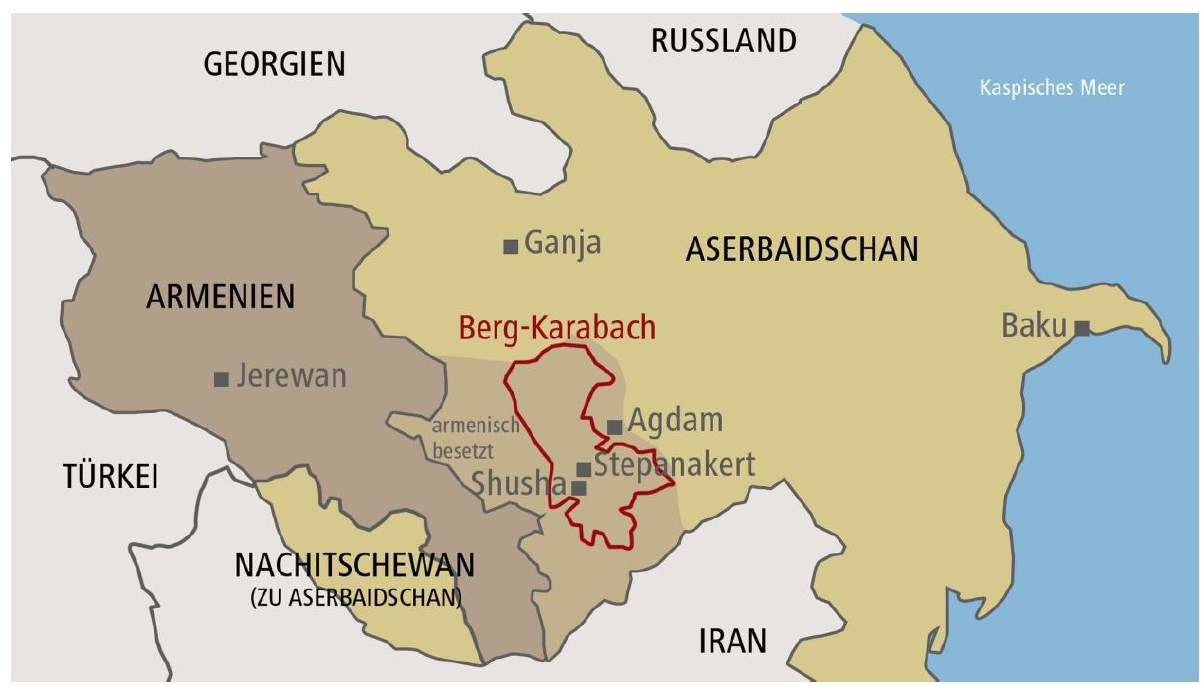
\includegraphics{images/karabach.png} \emph{Ausgangslage}

\subsubsection{Kriegsursachen}\label{kriegsursachen}

\begin{itemize}
	\tightlist
	\item
	      Ungelöster Territorialdisput (frozen conflict)
	\item
	      Militärische Aufrüstung
	\item
	      Aussenpolitik Türkei
	\item
	      Innenpolitische Spannungen in Aserbaidschan
\end{itemize}

\subsubsection{Kriegsauslöser}\label{kriegsausluxf6ser}

\begin{itemize}
	\tightlist
	\item
	      Grenzscharmützel (Jul.)
	\item
	      Militärübungen (Jul.~- Sep.)
	\item
	      Provokation von Schuscha (Aug.)
\end{itemize}

Aserbaidschansische Offensive, 27.09.2020, 8h03 (gem ARM)

Armenischer Beschuss gn Stellungen, 6h00 deshalb Gegenoffensive (gem
AZE)

\subsubsection{Kriegsparteien}\label{kriegsparteien}

\begin{itemize}
	\tightlist
	\item
	      Aserbaidschan hohes Budget, bessere Ausrüstung, Drohnen
	\item
	      Armenien hat etwa gleich viel Soldaten, technisch unterlegen
\end{itemize}

\subsubsection{ODKB}\label{odkb}

\begin{itemize}
	\tightlist
	\item
	      Militärisches Bündnis um Russland
	\item
	      Armenien ist Teil davon
	\item
	      Armenien hat sich dem Westen zugewannt
	\item
	      Russland hat militärisch nicht interveniert
\end{itemize}

(Reihenfolge der letzten zwei Punkte unklar)

\subsubsection{Konfliktverlauf}\label{konfliktverlauf}

\begin{itemize}
	\tightlist
	\item
	      Kurz, 27.09.20-10.11.20
\end{itemize}

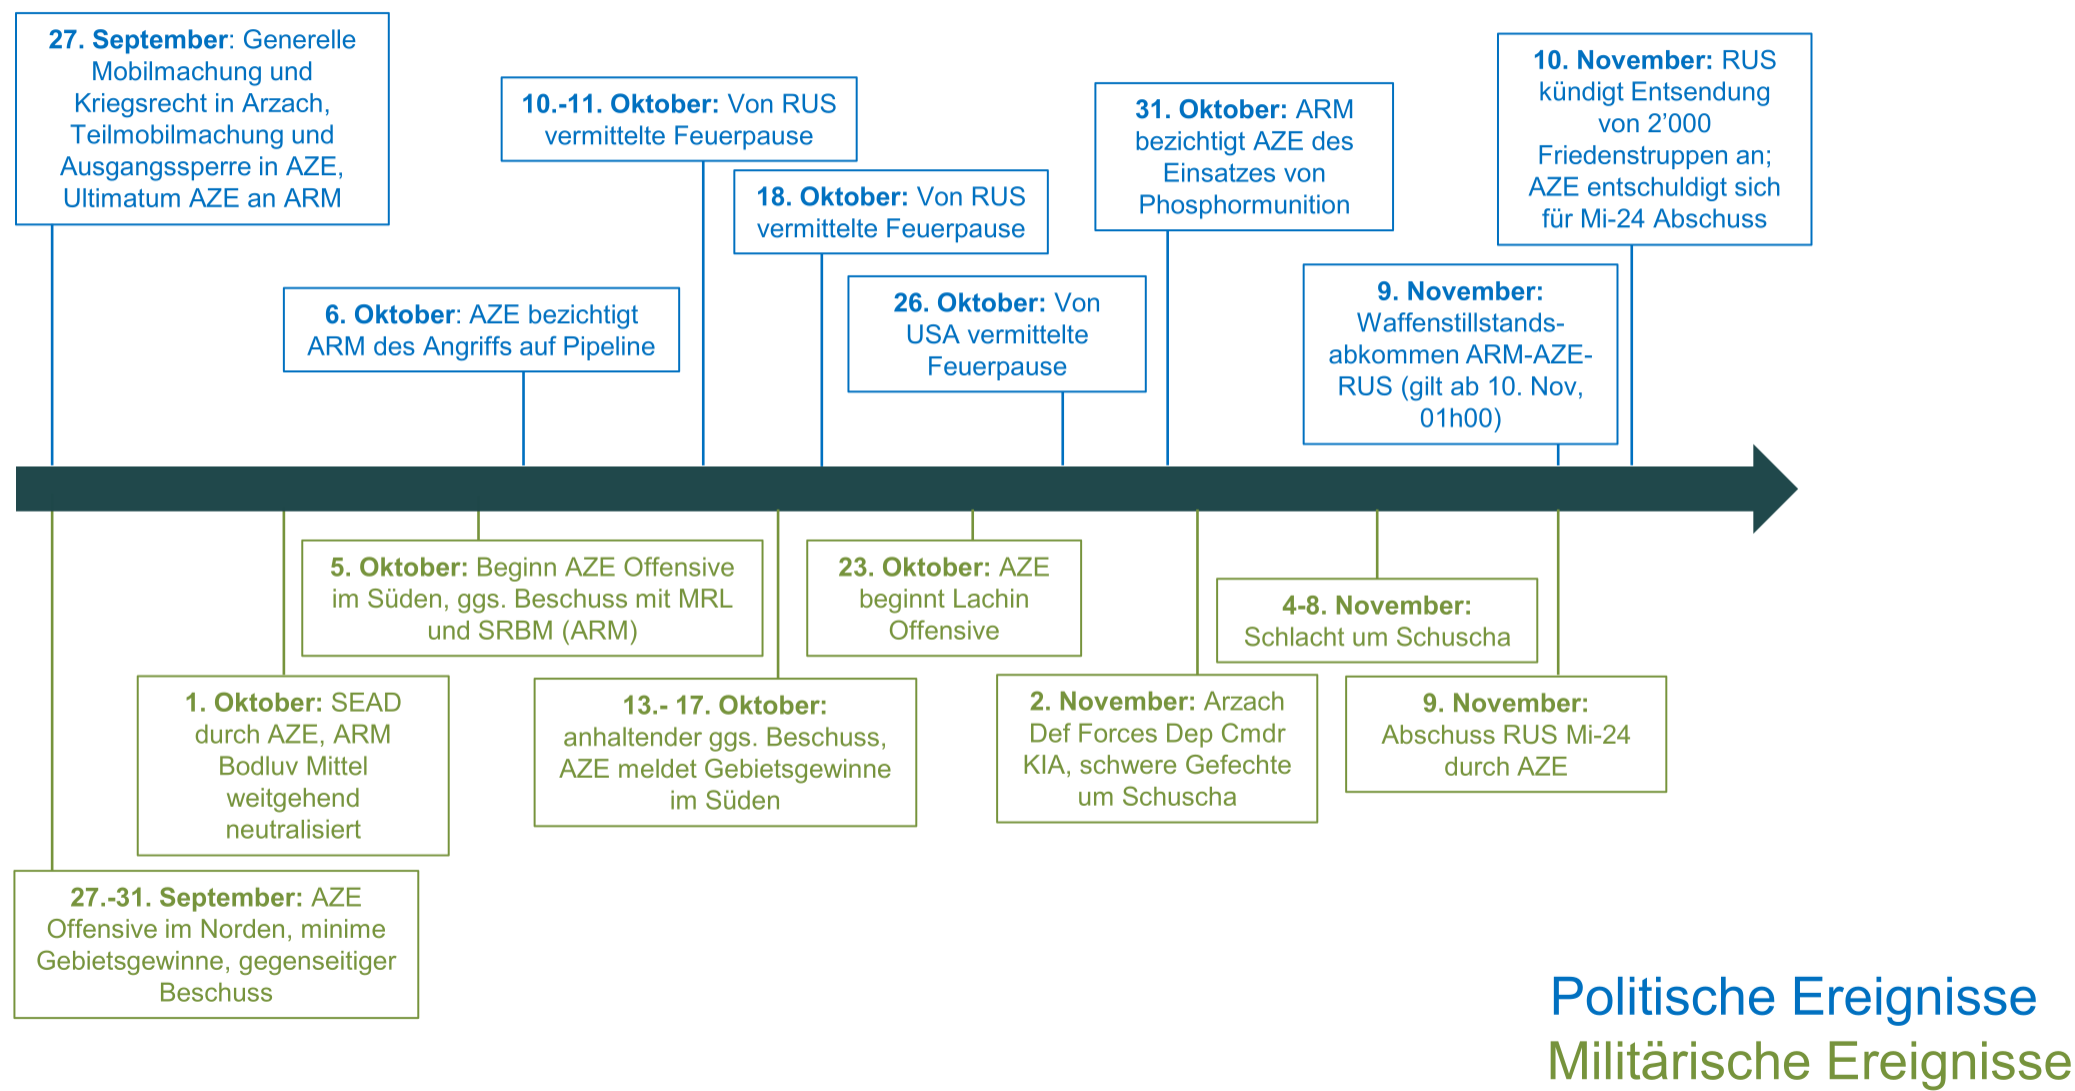
\includegraphics{images/verlauf-karabach.png} \emph{CAPTION}

\subsubsection{Waffenstillstand}\label{waffenstillstand}

\begin{itemize}
	\tightlist
	\item
	      Stadt Schuscha auf Hügel an strategisch wichtiger Lage
	\item
	      Schnelle Einnahme durch Aserbaidschan
	\item
	      Darauffolgend der Waffenstillstand
\end{itemize}

\subsubsection{Rückeroberung Bergkarabach
	2023}\label{ruxfcckeroberung-bergkarabach-2023}

\begin{itemize}
	\tightlist
	\item
	      Seit Dezember 2022: Blockade der Republik Arzach durch AZE
	\item
	      19.09.2023: AZE bricht Waffenstillstand und greift Republik Arzach an
	\item
	      20.09.2023: Waffenstillstand unter russischer Vermittlung
	\item
	      Verdacht auf ethnische Säuberungen und Völkermord an der armenischen
	      Bevölkerung
	\item
	      Flucht von über 100 000 armenischen Zivilisten
\end{itemize}

\subsubsection{Fazit}\label{fazit-4}

\begin{itemize}
	\tightlist
	\item
	      Gekränkte Verlierer sind gefährliche Nachbaren, da sie auf Revanche
	      aus sind (siehe Aserbaidschan)
	\item
	      Externe Unterstützung kann kriegsentscheidend sein, ähnlich wie die
	      Ausnutzung von Gelegenheitsfenstern (durch Aserbaidschan 2020 und
	      2023)
	\item
	      Angriffsdrohnen ermöglichten Aserbaidschan die Schwächung der
	      armenischen Verteidigung
	\item
	      Traditionelle Luftverteidigung ist unzureichend, um gegen
	      Angriffsdrohnen bestehen zu können
	\item
	      Glaubwürdigkeit der Organisation des Vertrags über kollektive
	      Sicherheit und Russlands als Schutzmacht (Armeniens) als Folge des
	      Nichteingreifens geschwächt
	\item
	      Lage in der Region bleibt volatil (Aliyev und Erdogan wollen
	      Verbindung der Turk-Völker über Sangesur-Korridor, Iran will das
	      verhindern, da einzige Landverbindung zu Russland)
\end{itemize}

\subsection{Der Ukrainekrieg}\label{der-ukrainekrieg}

\subsubsection{Leitfragen}\label{leitfragen-9}

\begin{itemize}
	\tightlist
	\item
	      Welche Ziele verfolgen die beiden Parteien im Ukrainekrieg?
	\item
	      Wie hat sich die militärische Lage in den letzten drei Jahren
	      verändert?
	\item
	      Welche Rolle kommt dem globalen Süden zu?
\end{itemize}

\begin{quote}
	Der Krieg ist das Gebiet der Ungewissheit, drei Vierteile derjenigen
	Dinge, worauf das Handeln im Kriege gebaut wird, liegen im Nebel einer
	mehr oder weniger grossen Ungewissheit. Hier ist es also zuerst, wo ein
	feiner, durchdringender Verstand in Anspruch genommen wird, um mit dem
	Takte {[}des{]} Urteils die Wahrheit herauszufühlen.\\
	- \emph{Carl von Clausewitz, Vom Kriege, Buch I, 3. Kapitel}
\end{quote}

\subsubsection{Lektüre}\label{lektuxfcre-9}

\begin{itemize}
	\tightlist
	\item
	      Franz-Stefan Gady/Michael Kofman, Ukraine's Strategy of Attrition, in:
	      Survival, Vol. 65 (2), 2023, S. 7-18.
	\item
	      Walerij Saluschnyj, On the Modern Design of Military Operations in the
	      Russo- Ukrainian War: In the Fight for the Initiative, 1. Februar
	      2024,
	      \href{https://s3.documentcloud.org/documents/24400154/ukraine-valerii-zaluzhnyi-essaydesign-of-war.pdf}{Artikel}
\end{itemize}

\subsubsection{Vorgeschichte}\label{vorgeschichte-1}

\begin{longtable}[]{@{}
	>{\raggedleft\arraybackslash}p{(\columnwidth - 2\tabcolsep) * \real{0.1053}}
	>{\raggedright\arraybackslash}p{(\columnwidth - 2\tabcolsep) * \real{0.8947}}@{}}
	\toprule\noalign{}
	\begin{minipage}[b]{\linewidth}\raggedleft
		Datum
	\end{minipage} & \begin{minipage}[b]{\linewidth}\raggedright
		                 Ereignis
	                 \end{minipage}                                                 \\
	\midrule\noalign{}
	\endhead
	\bottomrule\noalign{}
	\endlastfoot
	12.1991                                    & Referendum über Unabhängigkeit von Russland                    \\
	12.1994                                    & Budapester Memorandum                                          \\
	12.2004                                    & Präsidentschaftswahl (``Orange Revolution'')                   \\
	01.2010                                    & Wahl des prorussischen Präsidenten Wiktor Janukowitsch         \\
	11.2013                                    & Beginn ``Euromaidan''-Proteste                                 \\
	02.2014                                    & Flucht und Absetzung Janukowitschs                             \\
	03.2014                                    & Besetzung der Krim durch Russland, Beginn des Krieges in der
	Ostukraine                                                                                                  \\
	07.2014                                    & Abschuss eines Passagierfliegers der Malaysia Airlines         \\
	02.2015                                    & Minsker Abkommen                                               \\
	2017                                       & Ukrainisches Parlament einigt sich auf NATO-Mitgliedschaft als
	aussenpolitisches Ziel                                                                                      \\
	05.2019                                    & Wahl Wolodymyr Selenskyi zum Präsidenten der Ukraine           \\
	21.02.2022                                 & Russland anerkennt die Volksrepubliken Donezk und Luhansk
	als unabhängig                                                                                              \\
	22.02.2022                                 & USA, EU und Verbündete sanktionieren Russland                  \\
	23.02.2022                                 & Putin kündigt eine militärische Spezialoperation an            \\
	24.02.2022                                 & Selenskyi ruft den Kriegszustand aus                           \\
\end{longtable}

\subsubsection{Krieg als Mittel der russischen Aussen- und
	Innenpolitik}\label{krieg-als-mittel-der-russischen-aussen--und-innenpolitik}

\begin{itemize}
	\tightlist
	\item
	      Zweiter Tschetschenienkrieg 1999-2009
	\item
	      Kaukasuskrieg 2008
	\item
	      Annexion Krim, Krieg im Donbass 2014
	\item
	      Syrienkrieg 2015 - heute?
\end{itemize}

\subsubsection{Kriegsziele Russlands}\label{kriegsziele-russlands}

\begin{itemize}
	\tightlist
	\item
	      Offiziell erklärt

	      \begin{itemize}
		      \tightlist
		      \item
		            Verhinderung Genozid im Donbass
		      \item
		            Demilitarisierung und ``Entnazifizierung'' Ukraine
	      \end{itemize}
	\item
	      Tatsächlich/verdeckt

	      \begin{itemize}
		      \tightlist
		      \item
		            Regierungsumsturz
		      \item
		            Abkopplung Ukraine von NATO/EU, Schaffung Pufferzone
		      \item
		            Wahrung russischer Einflussbereich
	      \end{itemize}
\end{itemize}

\subsubsection{Kriegsbeginn Winter-Frühling
	2022}\label{kriegsbeginn-winter-fruxfchling-2022}

\begin{itemize}
	\tightlist
	\item
	      Russische Hauptstösse auf vier Angriffsachsen
\end{itemize}

\begin{figure}
	\centering
	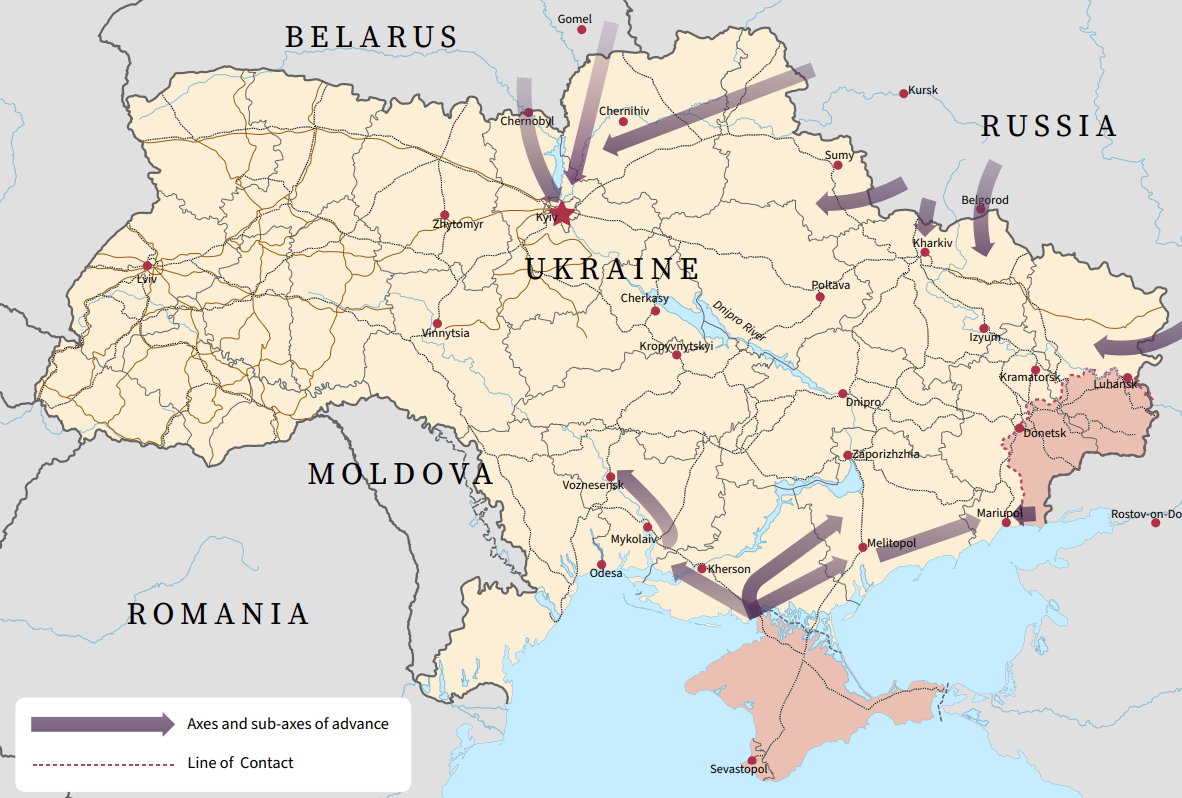
\includegraphics{images/ua22.png}
	\caption{ua22}
\end{figure}

\subsubsection{Erkenntnisse nach
	Angriff}\label{erkenntnisse-nach-angriff}

\begin{itemize}
	\tightlist
	\item
	      Schwere Verletzung des Völkerrechts durch Russland, beschränkter Wert
	      von Abkommen und Bündnissen
	\item
	      Rohstoffabhängigkeit des Westens von Russland als Nachteil bei
	      Verhängung von Sanktionen
	\item
	      Wirtschaftssanktionen waren nur von beschränkter Wirkung
	\item
	      Aufmarsch und Vorbereitung der russischen Streitkraft nahmen 3-4
	      Monate in Anspruch
	\item
	      Angriff erfolgte entlang der gesamten Grenze (Norden, Osten, Süden)
	      und verlief konzentrisch Richtung Hauptstadt
	\item
	      ``Hybride'' Kriegsführung war nur mit starker konventioneller
	      Komponente wirksam
\end{itemize}

\subsubsection{Strategiewechsel Sommer-Herbst
	2022}\label{strategiewechsel-sommer-herbst-2022}

\begin{itemize}
	\tightlist
	\item
	      Fokus Donbass
\end{itemize}

\subsubsection{Gescheiterte Ukrainische Gegenoffensive
	2023}\label{gescheiterte-ukrainische-gegenoffensive-2023}

\begin{itemize}
	\tightlist
	\item
	      Minimale Erfolge, hoher Verlust an Material und Personal
\end{itemize}

\begin{figure}
	\centering
	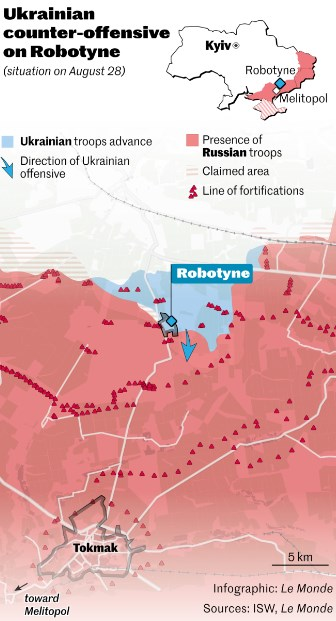
\includegraphics{images/tokmak.png}
	\caption{tokmak}
\end{figure}

\subsubsection{Stellungskrieg 2023}\label{stellungskrieg-2023}

\subsubsection{Weiter mit Stellungskrieg
	2024}\label{weiter-mit-stellungskrieg-2024}

\begin{itemize}
	\tightlist
	\item
	      2 Ausnahmen
\end{itemize}

\subsubsection{Frozen Conflict 2025?}\label{frozen-conflict-2025}

\begin{itemize}
	\tightlist
	\item
	      Keith Kellog Version: Entmilitarisierte Zone von westlichen
	      Friedenstruppen -ewacht
	\item
	      Stabilisierte Frontlinie gekoppelt an finanzielle und militärische
	      Unterstützung gegenüber der Ukraine
	\item
	      Über 1000 Kilometer lange Bufferzone
\end{itemize}

\begin{longtable}[]{@{}
	>{\raggedright\arraybackslash}p{(\columnwidth - 2\tabcolsep) * \real{0.5143}}
	>{\raggedright\arraybackslash}p{(\columnwidth - 2\tabcolsep) * \real{0.4857}}@{}}
	\toprule\noalign{}
	\begin{minipage}[b]{\linewidth}\raggedright
		Vorstellung USA
	\end{minipage} & \begin{minipage}[b]{\linewidth}\raggedright
		                 Vorstellung Russland
	                 \end{minipage} \\
	\midrule\noalign{}
	\endhead
	\bottomrule\noalign{}
	\endlastfoot
	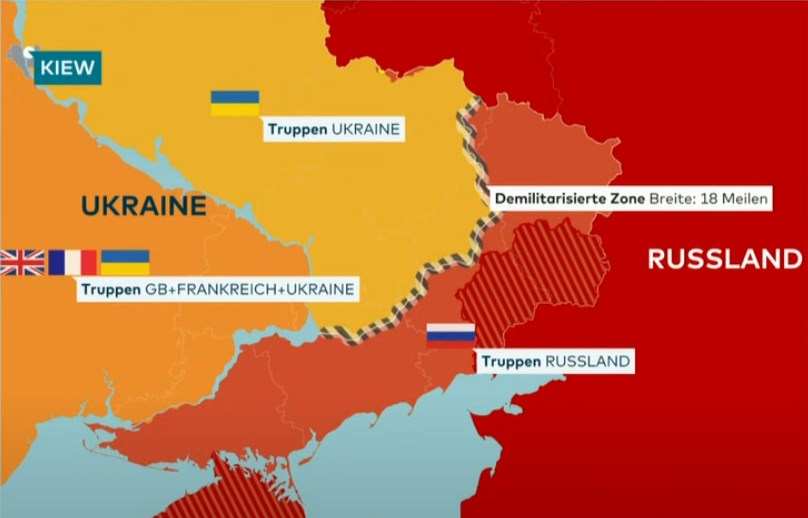
\includegraphics{images/buffer-usa.png}     &
	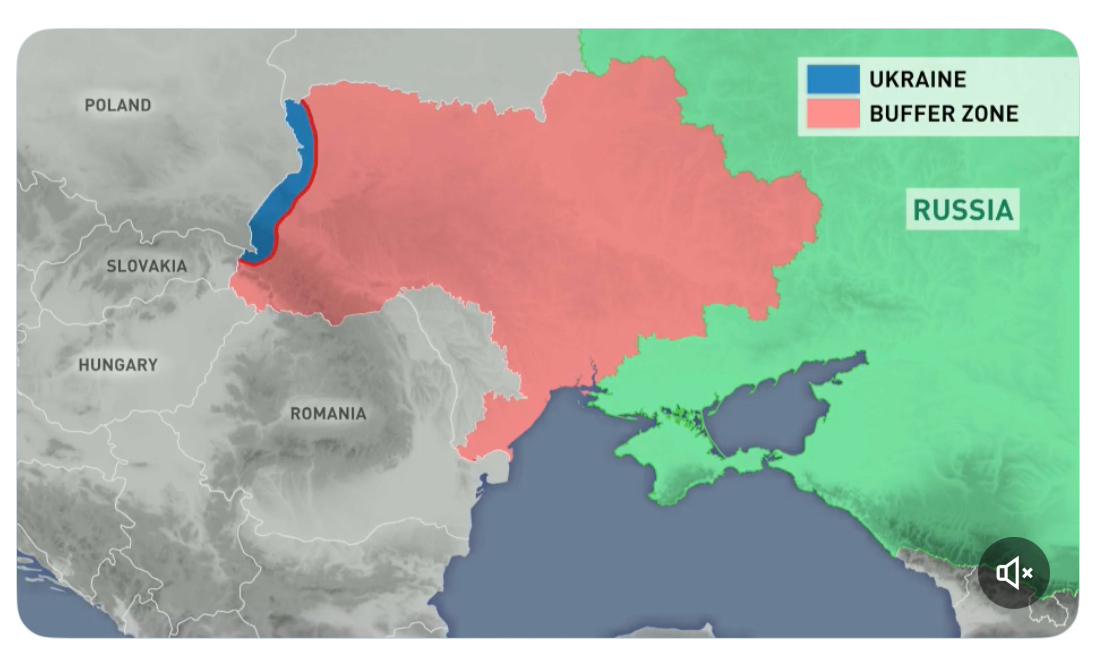
\includegraphics{images/buffer-rf.jpg}                      \\
\end{longtable}

\subsubsection{Diplomatische
	Auswirkungen}\label{diplomatische-auswirkungen}

\begin{itemize}
	\tightlist
	\item
	      FOTO BRICS-Treffen Südafrika 2023
	\item
	      Der amerikanische Ökonom Jim O'Neill sprach schon 2001 von BRICS
\end{itemize}

\subsubsection{Mögliche Entwicklung}\label{muxf6gliche-entwicklung}

\paragraph{Beschrieb}\label{beschrieb}

\begin{itemize}
	\tightlist
	\item
	      Voraussetzungen
\end{itemize}

\paragraph{Russland gewinnt Krieg}\label{russland-gewinnt-krieg}

\begin{itemize}
	\tightlist
	\item
	      Einstellen der Unterstützung der Ukraine durch den Westen
	\item
	      Kontinuierliche Unterstützung Russlands durch Partner
	\item
	      Ukraine geht Munition und Material aus
\end{itemize}

\paragraph{Sturz des Regimes in
	Russland}\label{sturz-des-regimes-in-russland}

\begin{itemize}
	\tightlist
	\item
	      Russische Gebietsverluste
	\item
	      Hohe russische Verluste
	\item
	      Verschärfung der Sanktionen
\end{itemize}

\paragraph{Waffenstillstand}\label{waffenstillstand-1}

\begin{itemize}
	\tightlist
	\item
	      Ukraine erleidet Rückschläge
	\item
	      Russland erobert weitere Gebiete
\end{itemize}

\paragraph{Ukraine gewinnt Krieg}\label{ukraine-gewinnt-krieg}

\begin{itemize}
	\tightlist
	\item
	      Russland muss sich aus allen besetzten Gebieten zurückziehen
	\item
	      Unterstützung der Ukraine hält an
	\item
	      Kein Eingreifen von russischen Verbündeten
	\item
	      Russland geht Munition, Material und qualifiziertes Personal aus
\end{itemize}

\paragraph{Russland setzt Massenvernichtungswaffen
	ein}\label{russland-setzt-massenvernichtungswaffen-ein}

\begin{itemize}
	\tightlist
	\item
	      Gebietsverluste Russlands
\end{itemize}

\paragraph{Abnutzungskrieg entlang langer Frontlinie
	-}\label{abnutzungskrieg-entlang-langer-frontlinie--}

\begin{itemize}
	\tightlist
	\item
	      Keiner Seite gelingt ein Durchbruch
	\item
	      Beide Seiten halten an Kriegszielen fest
\end{itemize}

\paragraph{NATO wird zur Kriegspartei}\label{nato-wird-zur-kriegspartei}

\begin{itemize}
	\tightlist
	\item
	      Russland setzt Massenvernichtungswaffen ein
	\item
	      Russland greift NATO direkt an
\end{itemize}

\subsubsection{Fazit}\label{fazit-5}

\begin{itemize}
	\tightlist
	\item
	      Der Ukrainekrieg wird in allen Domänen geführt.
	\item
	      Es lässt sich eine Abfolge von verschiedenen Kriegsphasen mit
	      wechselnden Dynamiken beobachten.
	\item
	      Derzeit findet auf der strategischen Ebene ein Abnutzungskrieg statt,
	      bei der die Kriegswirtschaft und die Unterstützung der Partner für
	      beide Seiten elementar ist.
	\item
	      Beide Seiten fürchten sich vor einer Eskalation, deshalb dürfte der
	      Abnutzungskrieg weitergehen.
\end{itemize}

\subsection{Israels Mehrfrontenkriege}\label{israels-mehrfrontenkriege}

\subsubsection{Leitfragen}\label{leitfragen-10}

\begin{itemize}
	\tightlist
	\item
	      Gegen welche Gegner kämpft Israel?
	\item
	      Wie gestaltet sich die strategische Kultur Israels?
	\item
	      Welche Rolle kommt der geographischen Lage Israels zu?
\end{itemize}

\subsubsection{Lektüre}\label{lektuxfcre-10}

\begin{itemize}
	\tightlist
	\item
	      Michel Wyss, The October 7 Attack: An Assessment of the Intelligence
	      Failings, in: CTC Sentinel, Vol. 17 (9), 2024, S. 1-7.
	\item
	      Azar Gat, The Aims of the War in Gaza - and the Strategy for Achieving
	      Them, 26.02.2024,
	      \href{https://www.inss.org.il/publication/gaza-war-targets/}{INSS}
\end{itemize}

\subsubsection{Geostrategische Lage}\label{geostrategische-lage}

\begin{itemize}
	\tightlist
	\item
	      Bewaffneter Konflikt seit Unabhängigkeitserklärung Israel im Mai 1948
	      (und bereits davor)
	\item
	      Übergang von regulären zwischenstaatlichen Kriegen zu irregulärer
	      Kriegführung
	\item
	      Diplomatische Initiativen mit Teilergebnissen, aber kein Durchbruch
	      bei Konfliktlösung
\end{itemize}

\subsubsection{Hamas (``Islamische
	Widerstandsbewegung'')}\label{hamas-islamische-widerstandsbewegung}

\begin{itemize}
	\tightlist
	\item
	      Gegründet 1987, Teil des globalen Muslimbruderschaftsnetzwerk
	\item
	      Selbstmordattentate während erster und zweiter Intifada
	\item
	      Sieg bei Parlamentswahlen 2006, Machtübernahme in Gaza 2007
	\item
	      Spannungen zwischen politischem und militärischem Flügel
\end{itemize}

\subsubsection{Ausgangslage vor dem
	7.10.2023}\label{ausgangslage-vor-dem-7.10.2023}

\begin{itemize}
	\tightlist
	\item
	      Politisch:

	      \begin{itemize}
		      \tightlist
		      \item
		            Verwaltung statt Lösung Palästinenserkonflikt
		      \item
		            Regionale Integration durch Normalisierung mit Golfstaaten
		      \item
		            Justizreform und Massenproteste
	      \end{itemize}
	\item
	      Militärisch:

	      \begin{itemize}
		      \tightlist
		      \item
		            Hamas und Hisbollah als lenkwaffen-basierte ``Terror- Armeen''
		      \item
		            Bisherige Verteidigungskonzeption nicht ausreichend
		      \item
		            Lösungsansatz: Investitionen in Bodentruppen und Sensor- Verbund
	      \end{itemize}
\end{itemize}

\subsubsection{Der strategische Schock vom
	7.10.2023}\label{der-strategische-schock-vom-7.10.2023}

\begin{itemize}
	\tightlist
	\item
	      Operation ``AL-AQSA FLOOD''

	      \begin{itemize}
		      \tightlist
		      \item
		            Ausschalten von Verteidigungs-, und Überwachungssysteme
		      \item
		            Vorrücken entlang gesamter Grenzlinie
	      \end{itemize}
	\item
	      07.10.2023 verlustreichster Tag in der Geschichte Israels

	      \begin{itemize}
		      \tightlist
		      \item
		            1195 Tote (darunter zwei CH-Doppelbürger)
		      \item
		            251 Personen nach Gaza entführt
	      \end{itemize}
\end{itemize}

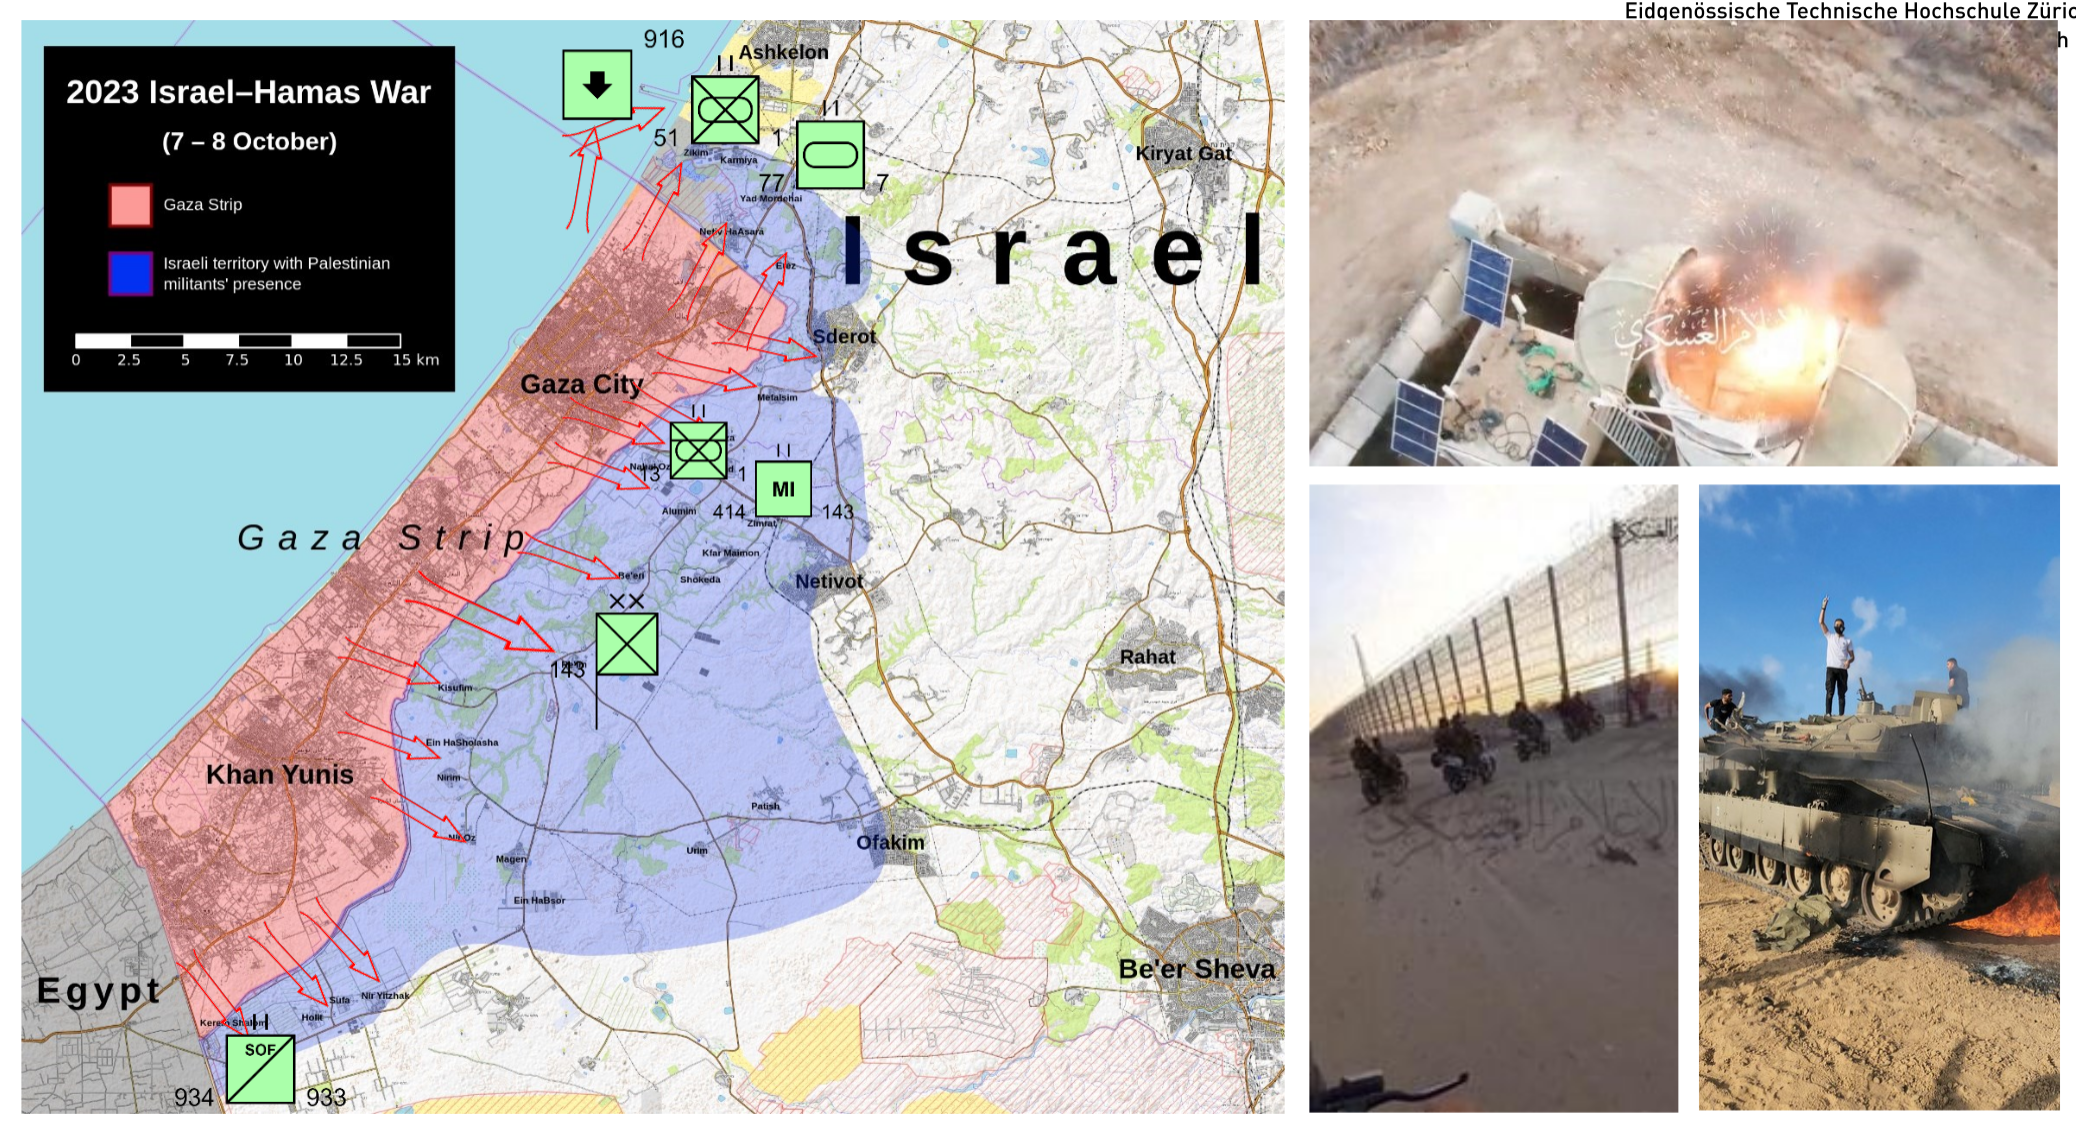
\includegraphics{images/al-aqsa.png} \emph{Ausmass und Taktiken der
	Al-Aqsa Flutwelle}

\subsubsection{Israelische Reaktion}\label{israelische-reaktion}

\begin{itemize}
	\tightlist
	\item
	      Op ``SWORDS OF IRON'' blutigster Konflikt in Gaza

	      \begin{itemize}
		      \tightlist
		      \item
		            Über 50'000 Palästinenser getötet, mindestens die Hälfte Zivilisten
		      \item
		            Humanitäre Katastrophe
	      \end{itemize}
	\item
	      Ziele Gemäss Regierung

	      \begin{itemize}
		      \tightlist
		      \item
		            Zerstörung Hamas
		      \item
		            Befreiung Geiseln
		      \item
		            Wiederherstellung Abschreckungsfähigkeit IDF
	      \end{itemize}
\end{itemize}

\subsubsection{Auswirkungen des
	Gazakrieges}\label{auswirkungen-des-gazakrieges}

\begin{itemize}
	\tightlist
	\item
	      Lokal

	      \begin{itemize}
		      \tightlist
		      \item
		            Eskalierende Spannungen und Gewalt im Westjordanland
		      \item
		            Wirtschaftliche Kosten
		      \item
		            Vertrauen in Regierung auf Tiefpunkt
	      \end{itemize}
	\item
	      Regional

	      \begin{itemize}
		      \tightlist
		      \item
		            Gefahr zweiter Front im Norden
		      \item
		            Indirekte Konfrontation mit Iran/Achse des Widerstands, insb.
		            Hisbollah und Huthi
		      \item
		            Normalisierung mit Saudi-Arabien sistiert, Spannungen mit regionalen
		            Partnern
	      \end{itemize}
	\item
	      Global

	      \begin{itemize}
		      \tightlist
		      \item
		            Einfluss USA auf Konfliktverlauf begrenzt
		      \item
		            ``Konkurrenz'' mit Krieg in Ukraine
		      \item
		            Polarisierung zwischen ``Westen'' und ``globalem Süden''?
	      \end{itemize}
\end{itemize}

\subsubsection{Einsatz von KI}\label{einsatz-von-ki}

\begin{itemize}
	\tightlist
	\item
	      Israel verwendet Künstliche Intelligenz ``Gospel'' (Infrastruktur) und
	      ``Lavender'' (Personen) zur automatisierten Zielgenerierung
	\item
	      Ca. 37'000 Personen waren auf automatisch generierten und von
	      menschlicher Seite bestätigten Tötungslisten seitens Israels
	\item
	      Früher hätten 20 ND-Spezialisten innerhalb von 300 Tagen ca. 20-30
	      Ziele generiert, mit der KI sind es in ca. 10 Tagen 200 Ziele (50x
	      mehr) (Die Berechnung geht irgendwie nicht ganz auf)
	\item
	      Hohe Zielgenerierung hat vermutlich zu mehr Beschuss in Gaza geführt
\end{itemize}

\subsubsection{Erneute Konfrontation in Gaza /
	Westjordanland}\label{erneute-konfrontation-in-gaza-westjordanland}

\begin{itemize}
	\tightlist
	\item
	      Januar bis März 2025: Waffenstillstand mit Hamas in Gaza
	      (Gefangenen-/Geiselaustausch)
	\item
	      März 2025: Israel beginnt erneut mit Beschuss von Gaza und warnt vor
	      erneutem Einmarsch und längerer Besetzung (mögl. als Druckmittel)
	\item
	      Westjordanland: IDF beschiesst seit Oktober 2023 regelmässig Ziele im
	      Westjordanland und hat dort seither über 10'000 Palästinenser
	      festgenommen
\end{itemize}

\subsubsection{Konfrontation mit Iran
	2024}\label{konfrontation-mit-iran-2024}

\begin{itemize}
	\tightlist
	\item
	      April: Israel bombardiert iranische Botschaft in Syrien und tötet
	      ranghohe iranische Militärs
	\item
	      April: Koordinierter Luftangriff Irans mit über 300 Drohnen und
	      Raketen. Israel: Luftangriffe gegen Ziele im Iran, Irak und Syrien
	\item
	      Juli und September: Israel tötet Haniyeh in Iran (Hamas Anführer) und
	      Nasrallah (Hisbollah Anführer)
	\item
	      Oktober: Iran beschiesst Israel mit über 200 Raketen in zwei Wellen.
	      Israelische Luftangriffe auf Iran
\end{itemize}

\subsubsection{Konfrontation mit Hisbollah
	(Libanon)}\label{konfrontation-mit-hisbollah-libanon}

\begin{itemize}
	\tightlist
	\item
	      Nach 7.10.2023 Angriff beginnt Hisbollah hauptsächlich militärische
	      Ziele in Israel zu beschiessen
	\item
	      Viele kleinere grenzüberschreitende Bodenangriffe und weitere
	      Raketenangriffe beider Seiten (steigende Zahl getöteter Zivilisten)
	\item
	      Sept.~und Okt. 2024: Operation «GRIM BEEPER»: «Pager-Attacke» auf
	      Hisbollah Ziele. Anschliessende Invasion Südlibanons durch IDF. Tötung
	      Nasrallahs (Hisbollah Chef)
	\item
	      Seit November 2024 unruhiger Waffenstillstand (öfters gebrochen)
\end{itemize}

\subsubsection{Konfrontation mit Syrien}\label{konfrontation-mit-syrien}

\begin{itemize}
	\tightlist
	\item
	      Dezember 2024: Netanyahu erklärt Waffenruhe mit Syrien als gebrochen
	      wegen Absetzung von Bashar al Assads Regime
	\item
	      Dezember 2024: Start der Operation ``ARROW OF BASHAN'': Besetzung der
	      demilitarisierten Golan Höhen und Raids bis nach Daraa
	\item
	      März 2025: Netanyahu droht bis ca. 2 km vor Damaskus vorzudringen
	\item
	      Ziel Israel: Demilitarisierung aller Gebiete südlich von Damaskus und
	      Zerstörung von syrischem Material
\end{itemize}

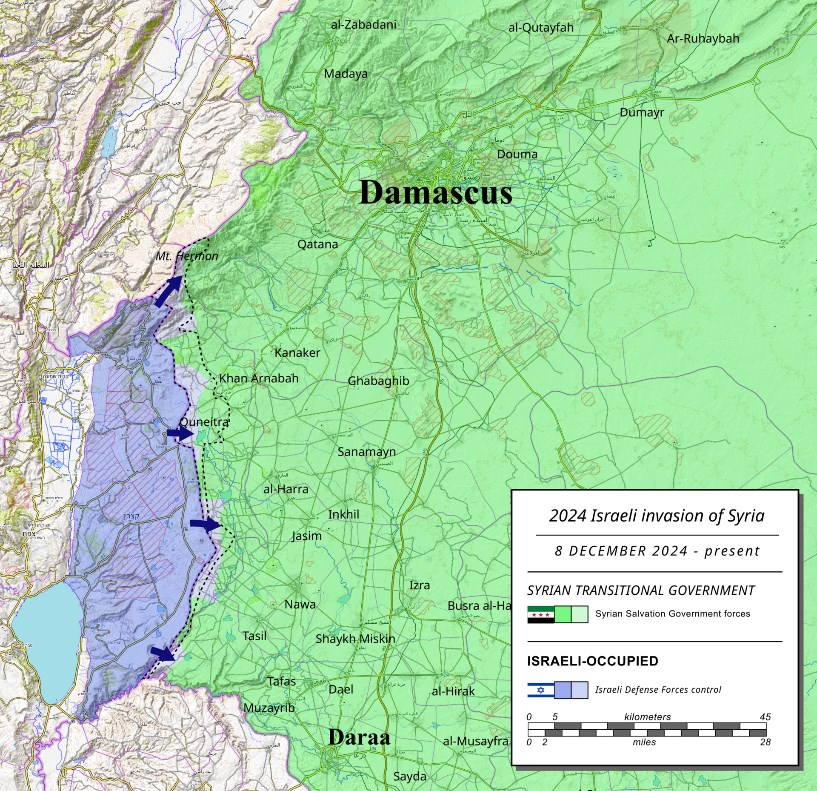
\includegraphics{images/damascus.png} \emph{Vorstoss Israels in Syrien}

\subsubsection{Konfrontation mit den Huthis
	(Jemen)}\label{konfrontation-mit-den-huthis-jemen}

\begin{itemize}
	\tightlist
	\item
	      Seit Oktober 2023 beschiessen Huthis regelmässig Schiffe im Roten Meer
	      und Ziele in Israel (oft mit iranischen Drohnen und Raketen)
	\item
	      Operation ``PROSPERITY GUARDIAN'': US geleitete multinationale
	      Koalition zur Abwehr von Huthi Angriffen
	\item
	      Juli 2024 und März 2025: Grössere Drohnenangriffe der Huthis auf Tel
	      Aviv und Jerusalem (Israel)
	\item
	      Wiederholte Luft- und Raketenangriffe von Israel und USA auf die
	      Huthis zeigen wenig Effekt
\end{itemize}

\subsubsection{Fazit}\label{fazit-6}

\begin{itemize}
	\tightlist
	\item
	      Israels vielschichtige Mehrfrontenkriege gehen weiter
	\item
	      Strategische Kultur der Offensive (ohne Verteidigung in der Tiefe)
	      prägt Israel
	\item
	      Latente Feindschaft Iran vs.~Israel beeinflusst den Nahen Osten
	      weiterhin. Derzeit hat Israel allerdings eine stärker Position als in
	      der Vergangenheit
	\item
	      Gaza: Von der Belagerung zur Okkupation
	\item
	      Westjordanland: Beide Seiten beschiessen einander regelmässig
	\item
	      Hisbollah: Nach ``Pager''-Angriff massgeblich geschwächt, brüchiger
	      Waffenstillstand
	\item
	      Iran: Die Luftangriffe hat Israel gemeinsam mit den Verbündeten
	      abgewehrt
	\item
	      Syrien: Israelische Intervention nach dem Fall Assads
	\item
	      Jemen: Latente Luftangriffe auf Huthi-Ziele
\end{itemize}

\subsection{Der syrische Bürgerkrieg und der Fall
	Assads}\label{der-syrische-buxfcrgerkrieg-und-der-fall-assads}

\subsubsection{Leitfragen}\label{leitfragen-11}

\begin{itemize}
	\tightlist
	\item
	      Welche Ziele verfolgten die verschiedenen Parteien im syrischen
	      Bürgerkrieg?
	\item
	      Weshalb wurde Assad im Dezember 2024 schnell gestürzt?
	\item
	      Wie könnte sich die humanitäre Lage in Syrien weiterentwickeln?
\end{itemize}

\subsubsection{Lektüre}\label{lektuxfcre-11}

\begin{itemize}
	\tightlist
	\item
	      Natasha Hall, With the Fall of Assad, Can Syria Rise?, in: Survival,
	      Vol. 67 (1), 2025, S. 45-54.
	\item
	      Christopher Phillips, The International System and the Syrian Civil
	      War, in: International Relations, Vol. 36 (3), 2022, 358-366, 374-377.
\end{itemize}

\subsubsection{Vorgeschichte Irak und
	Syrien}\label{vorgeschichte-irak-und-syrien}

\paragraph{Von JTJ zum ``Islamischen
	Staat''}\label{von-jtj-zum-islamischen-staat}

\begin{itemize}
	\tightlist
	\item
	      Jama'at al-Tawhid wal-Jihad 1999--2004
	\item
	      Al-Qaida im Irak (AQI) 2004--2006
	\item
	      Islamischer Staat des Irak (ISI) 2006--2013
	\item
	      ISIS(yrien) 2013-2014
	\item
	      Islamischer Staat seit Juni 2014

	      \begin{itemize}
		      \tightlist
		      \item
		            Ernennung von Kalif Abu Bakr Al-Baghdadi
	      \end{itemize}
\end{itemize}

\paragraph{Krieg 2014}\label{krieg-2014}

\subparagraph{Ursachen}\label{ursachen}

\begin{itemize}
	\tightlist
	\item
	      Jihadistisch-salafistische Ideologie
	\item
	      Konfessioneller Antagonismus (Schiiten vs.~Sunniten)
	\item
	      Diskriminierung sunnitischer Iraker, ``De-Ba'athifizierung''
	\item
	      Abzug US-Streitkräfte aus Irak
	\item
	      Territorialer Herrschaftsanspruch
\end{itemize}

\subparagraph{Auslöser}\label{ausluxf6ser}

\begin{itemize}
	\tightlist
	\item
	      Spaltung zwischen Jabhat al-Nusra und ISIS
	\item
	      Ausschluss von ISIS bei Al-Qaida (innerjihadistischer Konflikt)
	\item
	      ISIS-Offensive in Syrien und Nordirak (Einnahme von Mosul)
	\item
	      Genozid an Jesiden und Christen
	\item
	      Kriegsverbrechen, Terror und Schreckensherrschaft
\end{itemize}

\subsubsection{Kriegsparteien im syrischen
	Bürgerkrieg}\label{kriegsparteien-im-syrischen-buxfcrgerkrieg}

\begin{itemize}
	\tightlist
	\item
	      Assad-Regime

	      \begin{itemize}
		      \tightlist
		      \item
		            Syrische Arabische Armee SAA
		      \item
		            Hisbollah
		      \item
		            Iran (hauptsächlich Revolutionsgarden)
		      \item
		            Russland
	      \end{itemize}
	\item
	      Globale Dschihadbewegung

	      \begin{itemize}
		      \tightlist
		      \item
		            Islamischer Staat
		      \item
		            Tanzin Hurras al-Din
		      \item
		            zahlreiche kleinere Gruppierungen
	      \end{itemize}
	\item
	      Kurden, weitere Minderheiten

	      \begin{itemize}
		      \tightlist
		      \item
		            Volksverteidigungseinheiten YPG
		      \item
		            Assyrischer Militärrat
		      \item
		            Demokratische Kräfte Syrien SDF
	      \end{itemize}
	\item
	      Sunnitische Rebellengruppen

	      \begin{itemize}
		      \tightlist
		      \item
		            Syrische Nationale Armee SNA
		      \item
		            Ahrar ash-Sham
		      \item
		            Ha'yat Tahrir ash-Sham HTS
		      \item
		            Türkei
		      \item
		            Golf-Staaten
		      \item
		            Jordanien
	      \end{itemize}
\end{itemize}

\subsubsection{Syrische Rebellengruppe
	HTS}\label{syrische-rebellengruppe-hts}

\begin{itemize}
	\tightlist
	\item
	      Hai'at Tahrir asch-Scham
	\item
	      Ehemalige Al-Qaida-Mitgliedsorganisation, treibende Kraft der
	      syrischen Opposition
	\item
	      Angeführt vom 42-jährigen Abu Mohammed al-Julani
	\item
	      Die USA, die UNO und andere haben HTS als Terrorgruppe eingestuft
	\item
	      Ziele

	      \begin{itemize}
		      \tightlist
		      \item
		            Sturz Assad und Aufbau eines islamischen Staates
		      \item
		            Legitimität, Distanzierung von al-Qaida und Konsolidierung
	      \end{itemize}
\end{itemize}

\subsubsection{Syrische Nationale Armee
	SNA}\label{syrische-nationale-armee-sna}

\begin{itemize}
	\tightlist
	\item
	      Ging ursprünglich aus desertierten Soldaten hervor, die sich in der
	      Free Syrian Army (FSA) zusammenschlossen
	\item
	      Stark von der Türkei unterstützt
	\item
	      Ziele

	      \begin{itemize}
		      \tightlist
		      \item
		            Sturz des syrischen Regimes
		      \item
		            Kampf gegen kurdische Autonomiebestrebungen im Norden und Osten
		            Syriens
	      \end{itemize}
\end{itemize}

\subsubsection{Southern Operations Room}\label{southern-operations-room}

\begin{itemize}
	\tightlist
	\item
	      Erreichte nach dem Sturz Assads vor den HTS- Kämpfern Damaskus
	\item
	      Kämpfte im Süden Syriens gegen die Dschihadisten des IS
	\item
	      Netzwerk aus verschiedenen kleinen und Kleinstgruppen
	\item
	      Ziele

	      \begin{itemize}
		      \tightlist
		      \item
		            Sturz des syrischen Regimes
		      \item
		            Freies und vereintes Syrien
	      \end{itemize}
\end{itemize}

\subsubsection{Islamisten/Dschihadisten}\label{islamistendschihadisten}

\begin{itemize}
	\tightlist
	\item
	      Al-Kaida wollte Anfang der 2010er-Jahre Syrien als Rückzugsgebiet
	      nutzen, stiess jedoch ab 2014 auf den IS
	\item
	      Der IS wurde in seinem Kerngebiet südlich von Rakka durch eine
	      westliche Allianz besiegt
	\item
	      Künftige Rolle des IS in Syrien ist derzeit unklar
	\item
	      Laut dem Islamwissenschaftler Reinhard Schulze hat der IS noch 8.000 -
	      20.000 Kämpfer
	\item
	      Ziele:

	      \begin{itemize}
		      \tightlist
		      \item
		            Wiederaufbau des Kalifats
		      \item
		            Kontrolle von Ressourcen und Rekrutierung von Kämpfern
	      \end{itemize}
\end{itemize}

\subsubsection{Kurden}\label{kurden}

\begin{itemize}
	\tightlist
	\item
	      Zwei Lager:

	      \begin{itemize}
		      \tightlist
		      \item
		            Syrischen Demokratischen Kräfte (SDF)
		      \item
		            Volksverteidigungseinheiten (YPG)
	      \end{itemize}
	\item
	      YPG hat Verbindungen zur PKK (derzeit in Auflösung)
	\item
	      Während der Assad-Jahre wurde die YPG teilweise vom Regime geduldet
	\item
	      Ziele:

	      \begin{itemize}
		      \tightlist
		      \item
		            Autonomie und Selbstverwaltung in den nördlichen Gebieten
		      \item
		            Wahrung kurdischer Identität
		      \item
		            Föderalisierung Syriens
	      \end{itemize}
\end{itemize}

\subsubsection{Die alten Eliten des
	Regimes}\label{die-alten-eliten-des-regimes}

\begin{itemize}
	\tightlist
	\item
	      Alewitische Familie Assad regierte 54 Jahre lang mit der Baath-Partei
	\item
	      Stützte sich auf einen geheimdienstlich gelenkten Unterdrückungsstaat
	      mit sunnitischen Eliten
	\item
	      Syrische Armee war relativ schwach
	\item
	      Ziele:

	      \begin{itemize}
		      \tightlist
		      \item
		            Machterhalt und Unterdrückung der Proteste
		      \item
		            Sicherung alawitischer Machtbasis
	      \end{itemize}
\end{itemize}

\subsubsection{Türkei}\label{tuxfcrkei}

\begin{itemize}
	\tightlist
	\item
	      Mehrere grenzüberschreitende Operationen
	\item
	      Türkisches Vorgehen wurde in der Vergangenheit immer wieder kritisiert
	\item
	      Russische Unterstützung Assads als Rückschlag, trotzdem
	      ``Kooperation'' mit Russland ab 2016
	\item
	      Ziele:

	      \begin{itemize}
		      \tightlist
		      \item
		            Bekämpfung der Kurden und Verhinderung eines kurdischen Staates
		      \item
		            Bekämpfung IS
		      \item
		            Zu Beginn: Sturz Assads
		      \item
		            Kontrolle Flüchtlingsströme
	      \end{itemize}
\end{itemize}

\subsubsection{Situation auf dem Boden}\label{situation-auf-dem-boden}

\begin{figure}
	\centering
	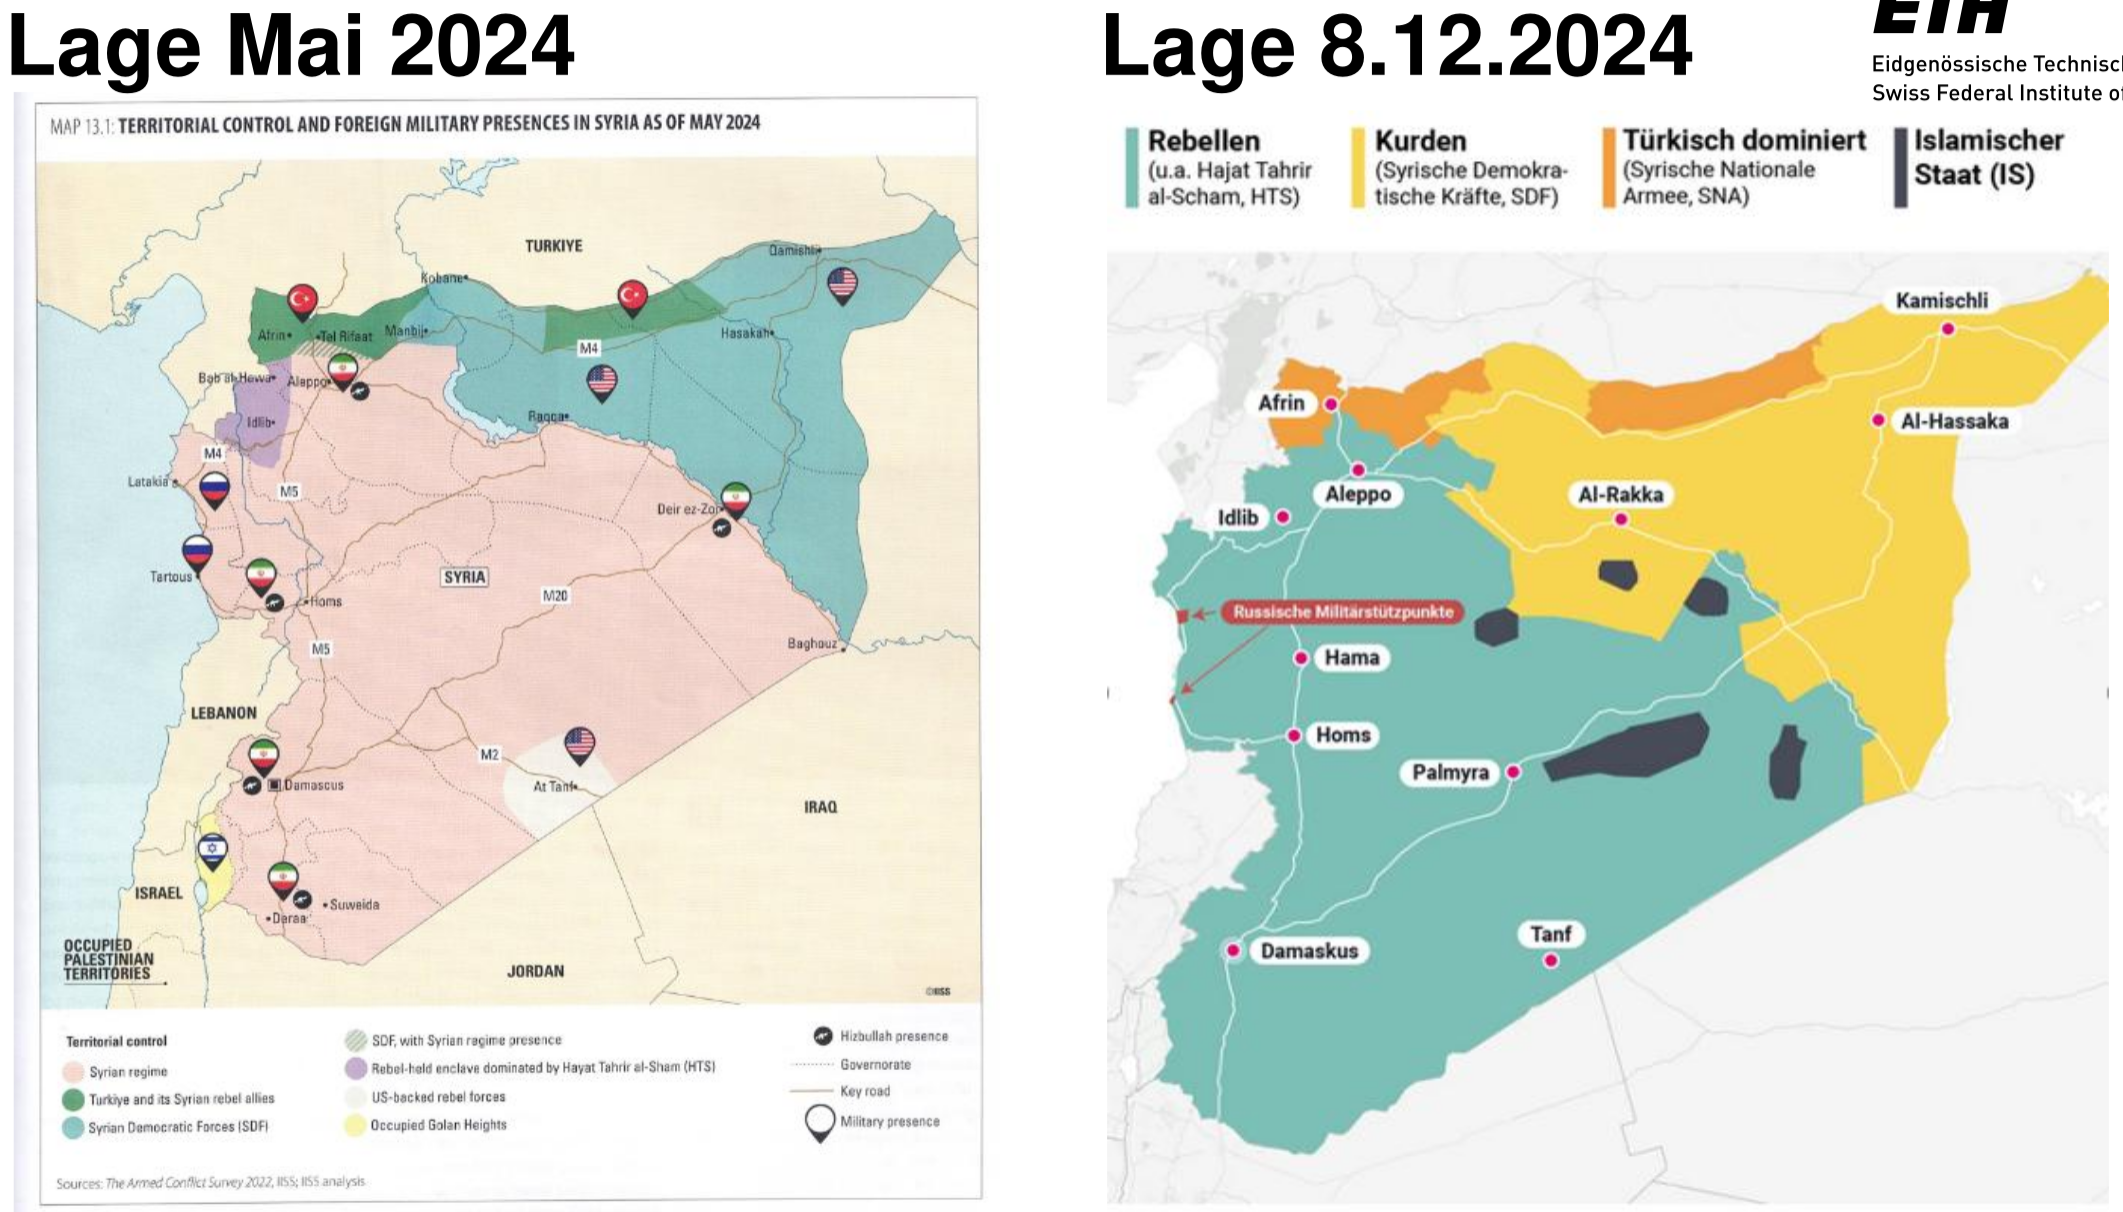
\includegraphics{images/syrien.png}
	\caption{syrien}
\end{figure}

\subsubsection{Anlage der Operation}\label{anlage-der-operation}

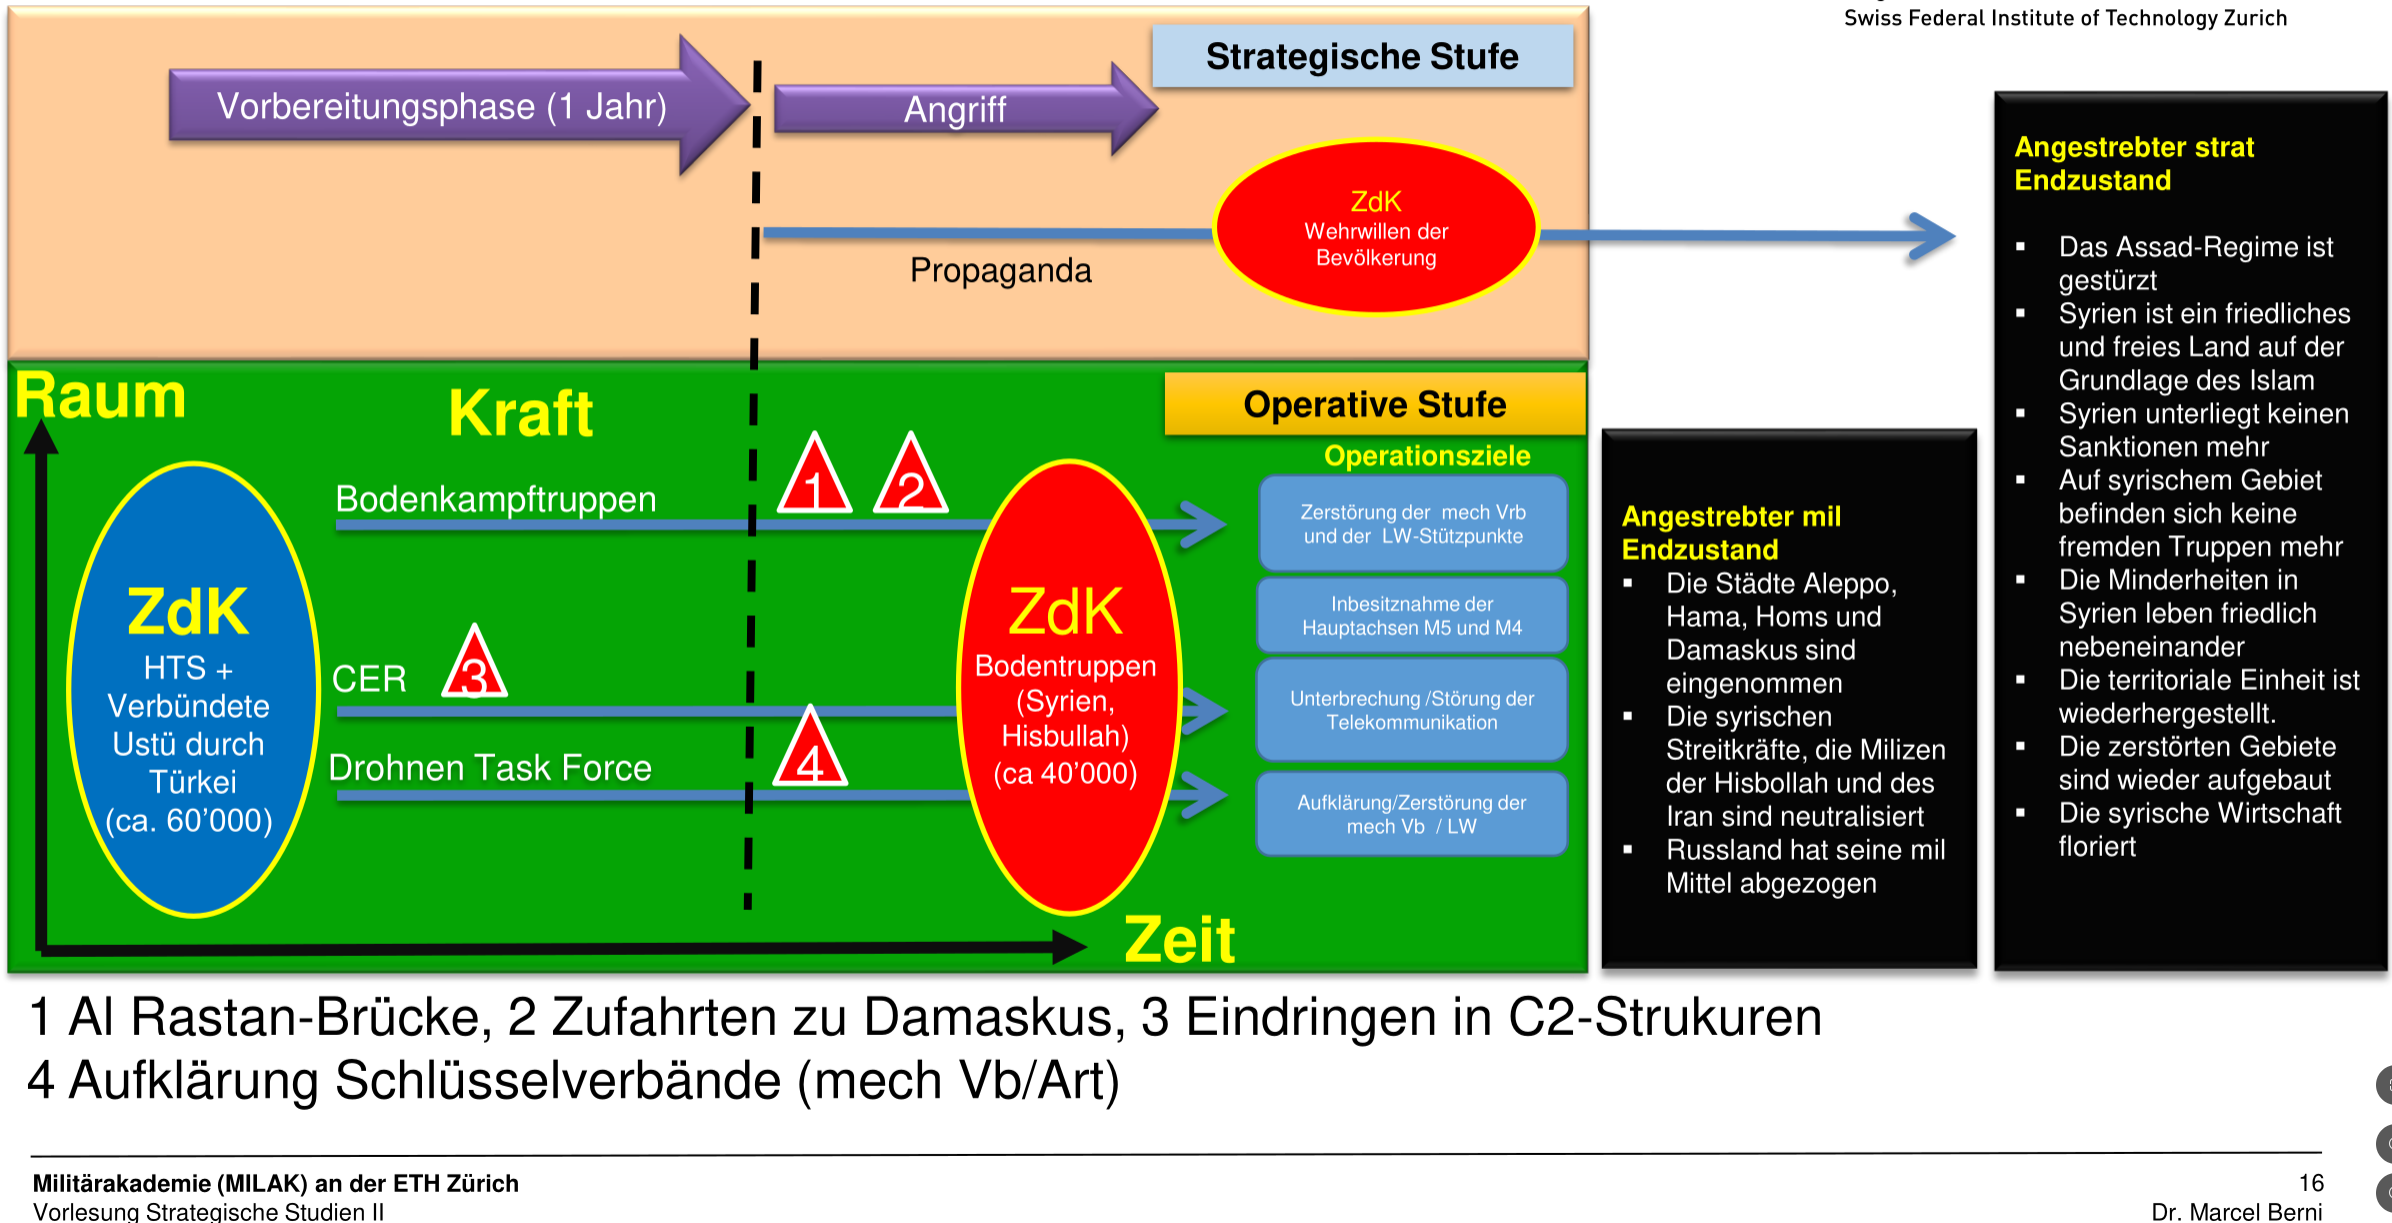
\includegraphics{images/strategie-hts.png} \emph{Strategisches Schema
	des von HTS geführten und mit Verbündeten umgesetzten Regimewechsels}

\subsubsection{Vier Szenarien}\label{vier-szenarien}

\paragraph{Teilung Syriens}\label{teilung-syriens}

\begin{itemize}
	\tightlist
	\item
	      Politische Stabilität durch Rebellen
	\item
	      Autonome Kurdengebiete
	\item
	      Anfang einer syrischen Föderation
	\item
	      Verbesserung humanitäre Lage
\end{itemize}

\paragraph{Kampf um die Kurdengebiete}\label{kampf-um-die-kurdengebiete}

\begin{itemize}
	\tightlist
	\item
	      Türkei unterstützt HTS
	\item
	      SNA greifen kurdische Gebiete an
	\item
	      IS erstarkt als Folge der Schwächung der Kurden
	\item
	      Verschlechterung humanitäre Lage
\end{itemize}

\paragraph{Zerstückelung}\label{zerstuxfcckelung}

\begin{itemize}
	\tightlist
	\item
	      Kein Gewaltmonopol
	\item
	      Zerfall in Gebiete unter Herrschaft lokaler Warlords
	\item
	      Anstieg Einfluss IS
	\item
	      Verschlechterung humanitäre Lage
\end{itemize}

\paragraph{Chaos}\label{chaos}

\begin{itemize}
	\tightlist
	\item
	      Rivalisierende Parteien
	\item
	      Angriff auf kurdische Gebiete
	\item
	      Erstarkung des IS
	\item
	      Katastrophale humanitäre Lage
\end{itemize}

\subsubsection{Fazit}\label{fazit-7}

\begin{itemize}
	\tightlist
	\item
	      Der syrische Bürgerkrieg begann 2011 im Rahmen des Arabischen
	      Frühlings
	\item
	      Der IS nutzte das vom Bürgerkrieg destabilisierte Syrien, um an
	      Einfluss, Kämpfer und Ressourcen zu gewinnen
	\item
	      Der IS verfolgte zu hochgesteckte, fanatische Ziele (ends), die sich
	      nicht mit den zur Verfügung stehenden Mitteln (means) und Methoden
	      (ways) erreichen liessen. Die angewandten Mittel bewirkten das
	      Gegenteil und stärkten die mannigfaltigen Gegner, die das Centrum
	      gravitatis (= Kontrolle des Territoriums) erfolgreich bekämpften.
	\item
	      Im November/Dezember 2024 gelang es der HTS mit türkischer
	      Unterstützung, die Assad-Dynastie nach über 50 Jahren Herrschaft mit
	      einer kurzen Blitzoffensive zu stürzen und den Bürgerkrieg (vorläufig)
	      zu beenden
\end{itemize}

\subsection{Chinas
	Grossmachtambitionen}\label{chinas-grossmachtambitionen}

mit MA Matthias Schachtler

\subsubsection{Leitfragen}\label{leitfragen-12}

\begin{itemize}
	\tightlist
	\item
	      Welche strategischen Ziele verfolgt die VR China?
	\item
	      Welche technologischen Innovationen nutzt China derzeit?
	\item
	      Welche Rolle kommt dabei Xi Jinping zu?
\end{itemize}

\subsubsection{Lektüre}\label{lektuxfcre-12}

\begin{itemize}
	\tightlist
	\item
	      Joel Wuthnow/M. Taylor Fravel, China's Military Strategy for a `New
	      Era': Some Change, More Continuity, and Tantalizing Hints, in: Journal
	      of Strategic Studies, 46 (6-7), 2023, S. 1149-1184.
\end{itemize}

\subsubsection{Chinas Grand Strategy}\label{chinas-grand-strategy}

\paragraph{Drei Theorien}\label{drei-theorien}

\begin{itemize}
	\tightlist
	\item
	      China hat keine Grand Strategy
	\item
	      Chinas Grand Strategy ist nur lokal (Taiwan, Japan, Indien, SCS)
	\item
	      Chinas Grand Strategy ist global (Belt and Road, Djibouti, etc.)
\end{itemize}

\paragraph{Grand Strategy global, aber militärisch
	lokal?}\label{grand-strategy-global-aber-milituxe4risch-lokal}

\begin{itemize}
	\tightlist
	\item
	      Deng Xiaoping: ``hide capabilities and bide time''
	\item
	      Das Traumatic Trifecta und der ``Neue Kalte Krieg''
	\item
	      Chinas Strategie für Deplazierung des US ``Hegemon'' (Doshi)

	      \begin{itemize}
		      \tightlist
		      \item
		            Blunting / Abstumpfen (1989 -- 2008)
		      \item
		            Building / Bauen (2008 -- 2016)
		      \item
		            Expanding / Expandieren (2016 -- jetzt)
	      \end{itemize}
\end{itemize}

\subsubsection{Strategie im
	Bürgerkrieg}\label{strategie-im-buxfcrgerkrieg}

\begin{itemize}
	\tightlist
	\item
	      Ende der Qing Dynastie; Nationalisten übernehmen (1912)
	\item
	      Gründung nationalistische Partei (1919)
	\item
	      Gründung CCP (1921) und PLA (1927)
	\item
	      Strategie im Bürgerkrieg (1927--1936, 1945--1949)

	      \begin{itemize}
		      \tightlist
		      \item
		            Active Defence (mobile Kriegsführung: Verteidigung, Bewegung,
		            Konter)
		      \item
		            Luring the Enemy in Deep (bekanntes Terrain, Ressourcen)
		      \item
		            People's War (Guerilla Kriegsführung, politische Kommissar)
	      \end{itemize}
	\item
	      Gründung People's Republic of China (1949) und Rückzug von Chiang
	      Kai-Sheks Nationalisten nach Taiwan (1949)
\end{itemize}

\subsubsection{Entwicklung Strategischer
	Richtlinien}\label{entwicklung-strategischer-richtlinien}

\begin{longtable}[]{@{}
	>{\raggedleft\arraybackslash}p{(\columnwidth - 2\tabcolsep) * \real{0.0588}}
	>{\raggedright\arraybackslash}p{(\columnwidth - 2\tabcolsep) * \real{0.9412}}@{}}
	\toprule\noalign{}
	\begin{minipage}[b]{\linewidth}\raggedleft
		Jahr
	\end{minipage} & \begin{minipage}[b]{\linewidth}\raggedright
		                 Doktrin in Schlagwort Zusammengefasst
	                 \end{minipage}                                             \\
	\midrule\noalign{}
	\endhead
	\bottomrule\noalign{}
	\endlastfoot
	1956                                       & ``Defending the motherland'' vs.~US                        \\
	1960                                       & ``Resist in the north, open in the south''                 \\
	1964                                       & ``Luring the enemy in the deep'' (by Mao)                  \\
	1977                                       & ``Active defense, luring the enemy in the deep''           \\
	1980                                       & ``Active Defense'' vs.~USSR, unofficial focus since 1969   \\
	1988                                       & ``Dealing with local wars and military conflicts''         \\
	1993                                       & ``Winning local wars under high-technology conditions''
	vs.~Taiwan                                                                                              \\
	2004                                       & ``Winning local wars under informatized conditions''       \\
	2014                                       & ``Winning informatized local wars'' (Xi Jinping in power)  \\
	2019                                       & ``Strategic guidelines for a new era'' (important shift or
	not?)                                                                                                   \\
\end{longtable}

\subsubsection{PLA und CCP-Führung}\label{pla-und-ccp-fuxfchrung}

\begin{longtable}[]{@{}lrr@{}}
	\toprule\noalign{}
	Name          & von        & bis             \\
	\midrule\noalign{}
	\endhead
	\bottomrule\noalign{}
	\endlastfoot
	Mao Zedong    & 1954       & 1976            \\
	Deng Xiaoping & 1979       & (oder 97?) 1993 \\
	Jiang Zemin   & 27.03.1993 & 15.03.2003      \\
	Hu Jintao     & 15.03.2003 & 14.03.2013      \\
	Xi Jinping    & 14.03.2013 & jetzt           \\
\end{longtable}

\begin{figure}
	\centering
	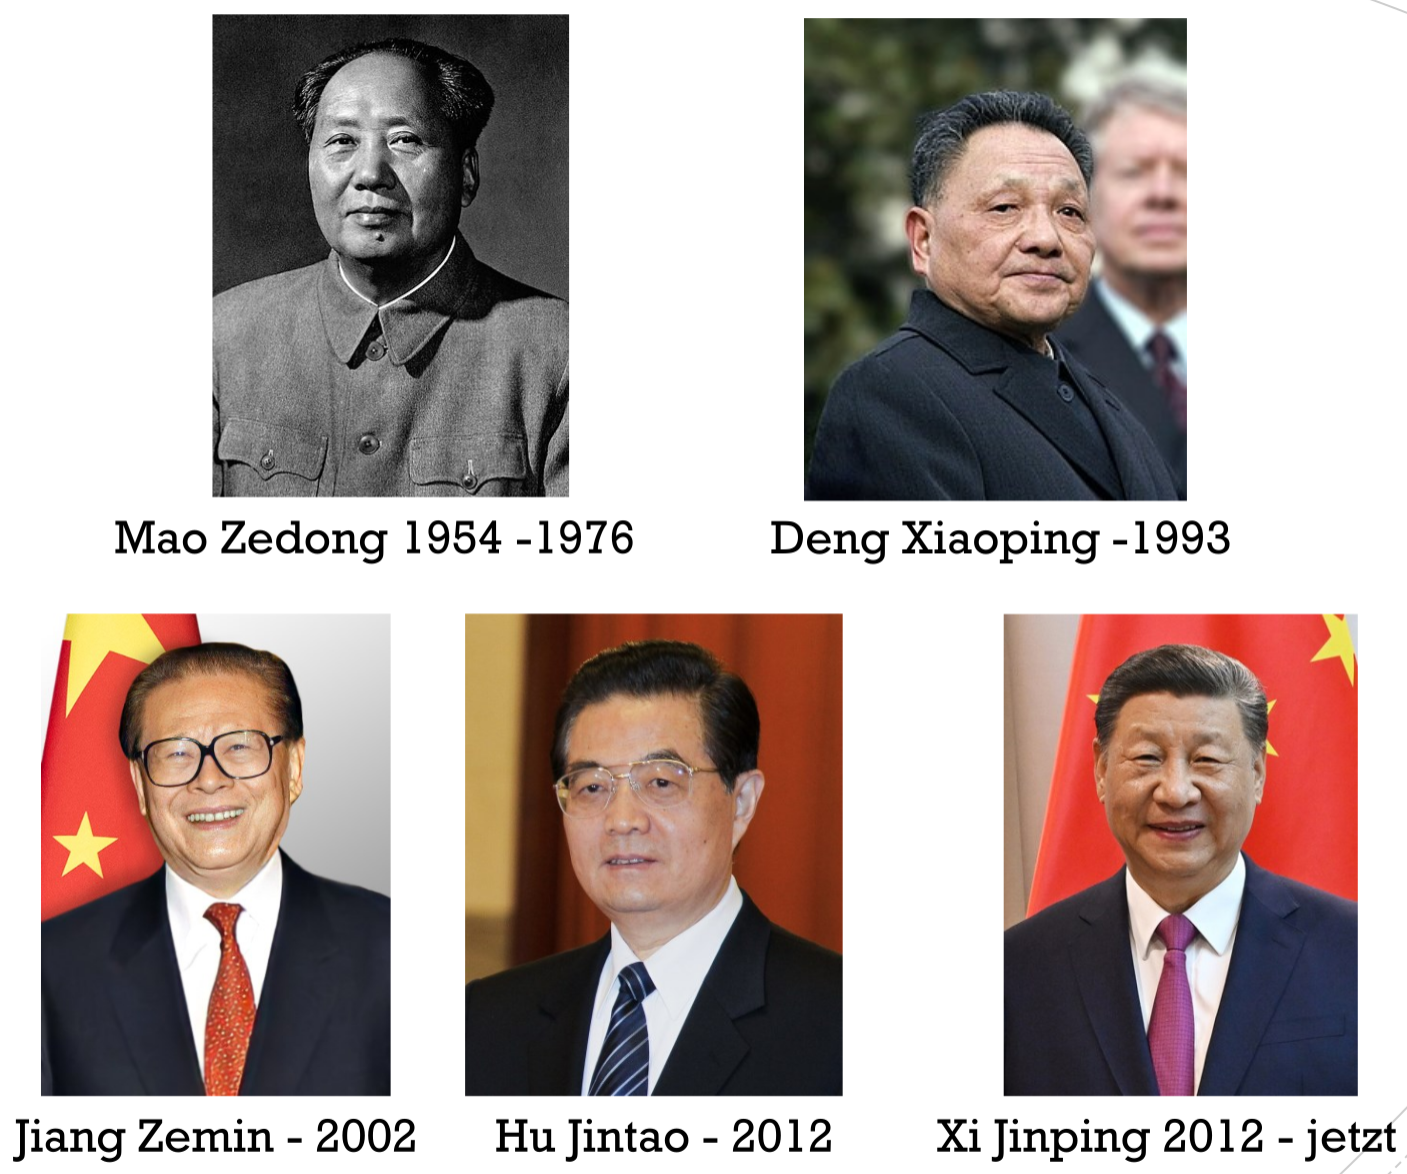
\includegraphics{images/kc.png}
	\caption{kc}
\end{figure}

\subsubsection{PLA Modernisierung unter Xi
	Jinping}\label{pla-modernisierung-unter-xi-jinping}

\paragraph{Ziele}\label{ziele}

\begin{itemize}
	\tightlist
	\item
	      Verschlankung der PLA
	\item
	      Loyalität gegenüber CCP und Xi
	\item
	      PLA soll ``red'' und ``expert'' sein
	\item
	      Korruptionsbekämpfung
	\item
	      Besser Joint-Operations
	\item
	      Modernisierung PLA-Material
\end{itemize}

\paragraph{2015 Reformen}\label{reformen}

\begin{itemize}
	\tightlist
	\item
	      Neue CMC-Aufstellung
	\item
	      Auflösung der General Departements
	\item
	      Reorganisation der Theatre Commands
	\item
	      Gründung der Strategic Support Force (spätere Abschaffung)
	\item
	      Kürzung von 300'000 Soldaten (Stärkung der Unteroffiziere)
\end{itemize}

\subsubsection{PLA heute}\label{pla-heute}

\begin{itemize}
	\tightlist
	\item
	      Verwaltung: Central Military Commission (CMC)
	\item
	      CMC-Führung: Xi Jinping
	\item
	      Budget 2025: 246 Milliarden \$ (?)
	\item
	      Wehrpflicht: Ja, aber hauptsächlich Freiwillige
	\item
	      Grösse: 2 Million aktiv, 500 000 Reserve\\
	      (plus 10 Millionen weitere bewaffnete Verbände)
\end{itemize}

\subsubsection{Militärstruktur Stand
	2025}\label{milituxe4rstruktur-stand-2025}

\paragraph{Four Services}\label{four-services}

\begin{itemize}
	\tightlist
	\item
	      Ground Force PLAGF (grün)
	\item
	      Navy PLAN (blau-weiss)
	\item
	      Air Force PLAAF (hellblau)
	\item
	      Rocket Force PLARF (gelb)
\end{itemize}

\paragraph{Four Arms (new)}\label{four-arms-new}

\begin{itemize}
	\tightlist
	\item
	      Aerospace Force
	\item
	      Cyberspace Force
	\item
	      Information Support
	\item
	      Joint Logistics Support
\end{itemize}

\paragraph{Weitere bewaffnete
	Verbände}\label{weitere-bewaffnete-verbuxe4nde}

\begin{itemize}
	\tightlist
	\item
	      People's Armed Forces Militia (8 Millionen)
	\item
	      Peoples Armed Police (PAP) (1,5 Millionen)
	\item
	      Coast Guard
\end{itemize}

\paragraph{Einteilung in 5
	Territorien}\label{einteilung-in-5-territorien}

\begin{figure}
	\centering
	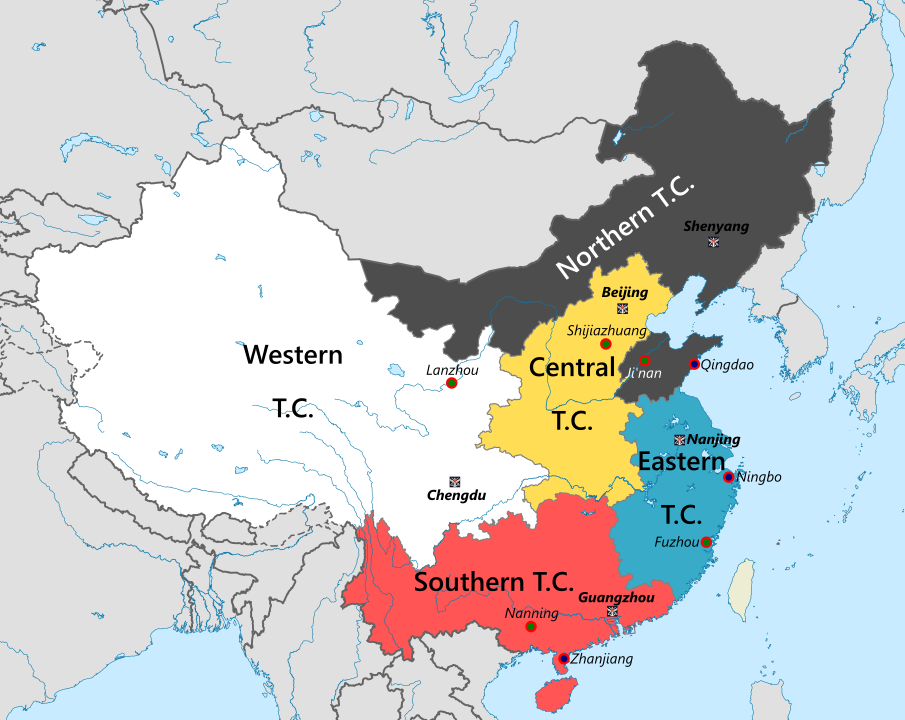
\includegraphics{images/china-territorial.png}
	\caption{china-territorial}
\end{figure}

\paragraph{Chinas Militär-Struktur}\label{chinas-milituxe4r-struktur}

\begin{figure}
	\centering
	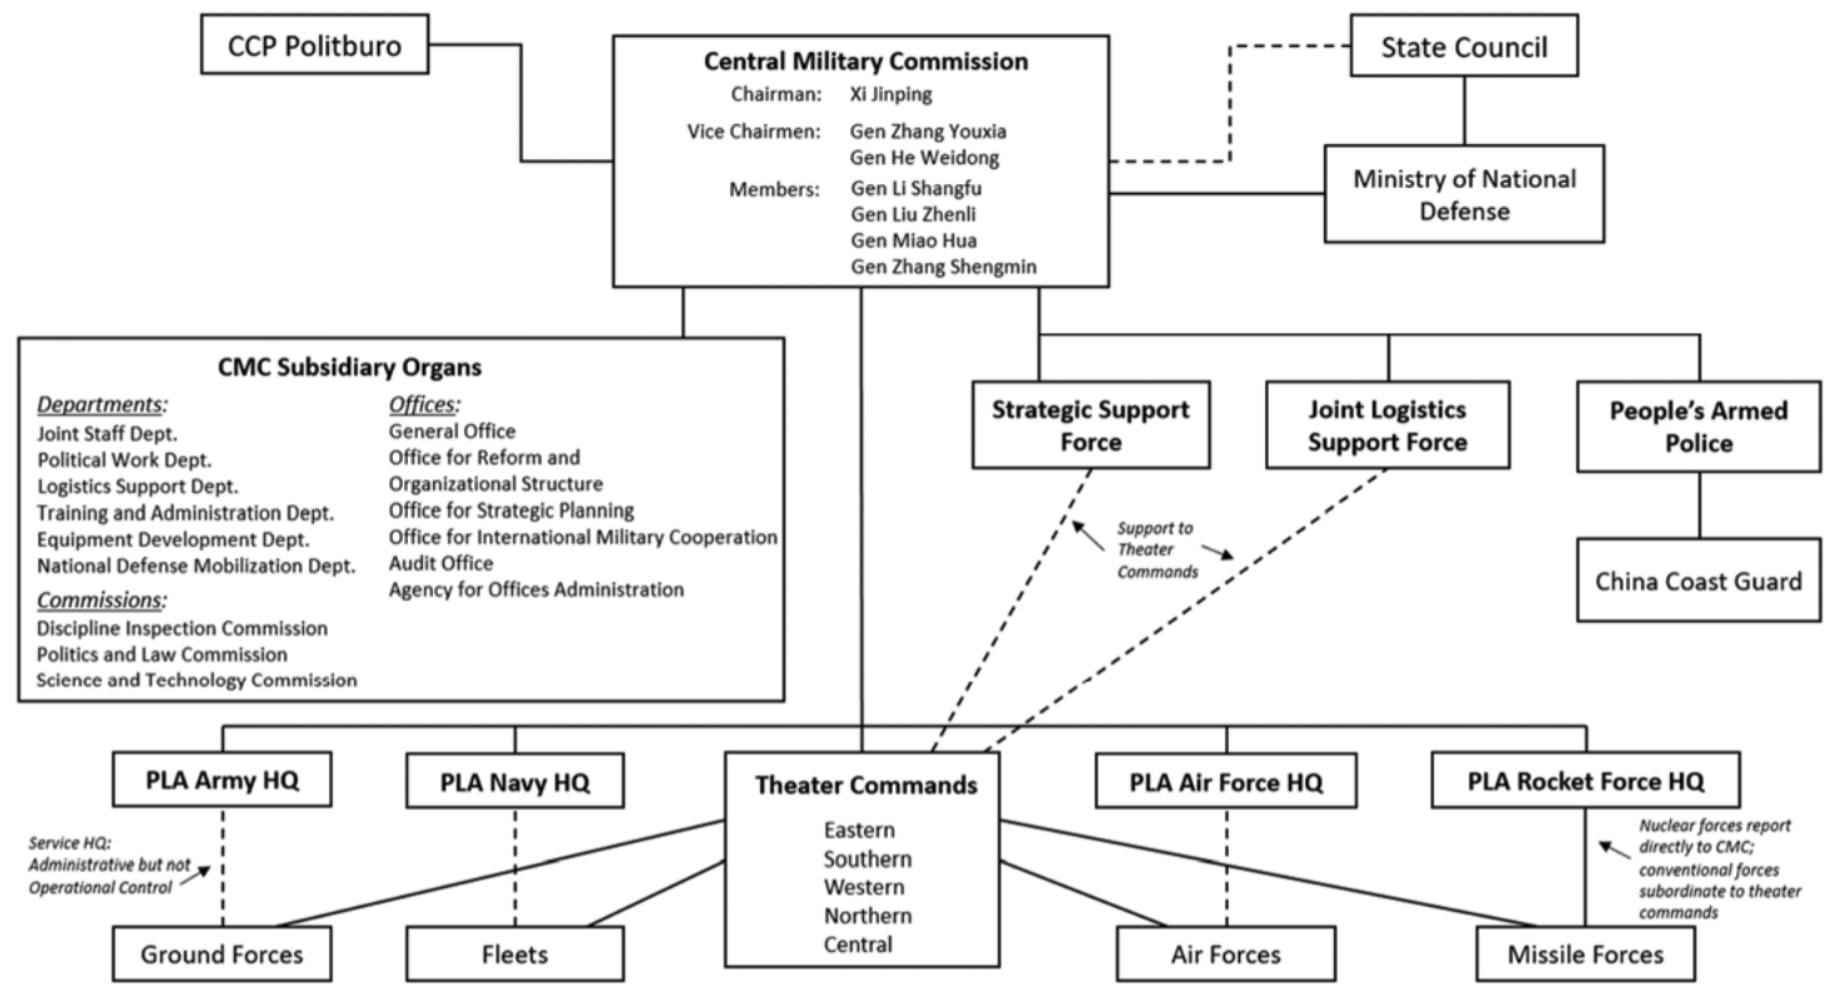
\includegraphics{images/china-struktur.png}
	\caption{china-struktur}
\end{figure}

\subsubsection{PLA Material
	Modernisierung}\label{pla-material-modernisierung}

\begin{itemize}
	\tightlist
	\item
	      Type 055 Cruiser
	\item
	      Dongfeng 21 ``Carrier Killer''
	\item
	      Shenyang J-35 Kampfjet
	\item
	      Fuijan Flugzeugträger
	\item
	      Landebrückenschiffe
	\item
	      Drohnenträgerdrohnen
\end{itemize}

\subsubsection{Krisen in der
	Taiwanstrasse}\label{krisen-in-der-taiwanstrasse}

\begin{itemize}
	\tightlist
	\item
	      1954 Erste Taiwanstrassenkrise (Bomb. Kinmen und Matsu)
	\item
	      1958 Zweite Taiwanstrassenkrise (Luft- und Seegefechte)
	\item
	      1994 Dritte Taiwanstrassenkrise (Lee Teng-Hui in USA)
	\item
	      2022 Vierte Taiwanstrassenkrise (Nancy Pelosi in Taiwan)
\end{itemize}

\subsubsection{Taiwan Invasion}\label{taiwan-invasion}

\begin{itemize}
	\tightlist
	\item
	      Beiping (Beijing) Modell für Invasion
	\item
	      Ausmass einer Taiwan Invasion

	      \begin{itemize}
		      \tightlist
		      \item
		            Operation Causeway (US Pläne japanisch kontrolliertes Taiwan zu
		            erobern mit 5 zu 1 Ratio)
		      \item
		            Operation Overlord (zuerst 160k, dann 800k Alliierte)
		      \item
		            Operation Iceberg (Schlacht um Okinawa mit 180k USA)
	      \end{itemize}
	\item
	      Schwierigkeiten der Invasion (Formation, Gezeiten etc.)
\end{itemize}

\subsubsection{China Taiwan Vergleich}\label{china-taiwan-vergleich}

\begin{itemize}
	\tightlist
	\item
	      China qualitativ und qualitativ in allen Bereichen deutlich überlegen
	\item
	      Taiwan mit starken geographischen Vorteilen
\end{itemize}

\subsubsection{Fazit}\label{fazit-8}

\begin{itemize}
	\tightlist
	\item
	      Chinesische Grossmachtambitionen scheinen realistisch
	\item
	      China momentan hauptsächlich regionale Militärmacht
	\item
	      Taiwan Invasion ist möglich aber extrem kostspielig
	\item
	      Schwierig einzuschätzen, wie kampftüchtig die PLA ist
\end{itemize}

\subsection{Überblickswerke zur
	Strategiegeschichte}\label{uxfcberblickswerke-zur-strategiegeschichte}

\begin{itemize}
	\tightlist
	\item[$\square$]
	      Jan Angstrom, J.J. Widen, Contemporary Military Theory: The Dynamics
	      of War, London 2015. {[} {]} John Baylis et al.~(Hg.), Strategy in the
	      Contemporary World. An Introduction to Strategic Studies, Oxford/New
	      York 2019.
	\item[$\square$]
	      Jeremy Black, Military Strategy. A Global History, New Haven 2020.
	\item[$\square$]
	      Hal Bands (Hg.), The New Makers of Modern Strategy, Princeton 2023.
	\item[$\square$]
	      Hervé Coutau-Bégarie, Traité de stratégie, Paris 2002.
	\item[$\square$]
	      Nathan K. Finney (Hg.), On Strategy. A Primer, Fort Leavenworth 2020.
	\item[$\square$]
	      Lawrence Freedman, Strategy. A History, New York 2013.
	\item[$\square$]
	      Beatrice Heuser, Den Krieg denken. Die Entwicklung der Strategie seit
	      der Antike, Paderborn 2010.
	\item[$\square$]
	      David Jordan et al., Understanding Modern Warfare, Cambridge 2016.
	\item[$\square$]
	      Thomas G. Mahncken, Joseph A. Maiolo (Hg.), Strategic Studies. A
	      Reader, London 2008.
	\item[$\square$]
	      Peter Paret (Hg.), Makers of Modern Strategy. From Machiavelli to the
	      Nuclear Age, Princeton 1986.
	\item[$\square$]
	      Elinor C. Sloan, Modern Military Strategy. An Introduction, Oxon/New
	      York 2017.
\end{itemize}

\subsection{Sprechstunden}\label{sprechstunden}

Sprechstundentermine können bei Bedarf individuell vereinbart werden.\\
Bitte setzen Sie sich mit dem Dozenten in Verbindung:
\href{mailto:marcel.berni@milak.ethz.ch}{\nolinkurl{marcel.berni@milak.ethz.ch}}
% \end{multicols}


\end{document}
